% !TEX root = slides_meat_30min_vpost.tex
% !TEX program = xelatex

\input{sty/header.tex}
\usepackage{sty/personalmacros}
\usepackage{sty/personalslides}

\usepackage{pifont}
\usepackage{multicol}
\usepackage{graphicx}
\usepackage{caption}
\usepackage{subcaption}
\usepackage{booktabs}

\usepackage{amssymb}
\usepackage{amsthm}
\usepackage{bbm}

\usepackage[spanish]{babel}
\usepackage{caption}
\captionsetup[table]{name=Tabla}
\captionsetup[figure]{name=Figura}

\newenvironment{wideitemize}{\itemize\addtolength{\itemsep}{10pt}}{\enditemize}
\definecolor{amaranth}{rgb}{0.9, 0.17, 0.31}

\title{{\color{yaleblue}\textbf{El Impacto del Cambio Climático en los Bienes Agrícolas}}}
\subtitle{\color{yaleblue}El Caso del Café}
\date{2026}
\author[Chacón]{\small Sebastián Chacón\inst{*}}
\institute[]{\inst{*} Universidad de Chile}

\begin{document}
\maketitle

\begin{frame}{Contenido}
\tableofcontents
\end{frame}
\section{Motivación}
\begin{frame}{Pregunta de investigación}
    \setbeamertemplate{itemize items}[circle]
    \begin{wideitemize}
        \item <1-> En mercados agrícolas, la exposición a temperaturas extremas (\textbf{estrés térmico}) puede deteriorar el desempeño de los cultivos, incrementando los costos marginales de producción.
        
        \item <2-> La literatura ha analizado este fenómeno como un choque agregado de productividad que genera adaptabilidad por parte los agentes.
        \begin{itemize}
            \item Métodos de forma reducida, datos de panel, \textit{long differences}
        \end{itemize}
        \item <3-> Pero el estrés térmico también puede tener efectos sobre la interacción estratégica de los productores en un mercado oligopólico.

        \item <4-> \textbf{\color{amaranth} ¿Cómo el estrés térmico reconfigura el equilibrio estratégico y el bienestar en el mercado internacional del café?}
    \end{wideitemize}
\end{frame}

\begin{frame}{En este trabajo}
    \setbeamertemplate{itemize items}[circle]
    \begin{wideitemize}
        \item <1-> Estimación estructural del mercado internacional del café, bajo un modelo de competencia \textit{à la Stackelberg}

        \item <2-> Estimación del impacto del estrés térmico en 1990-2019. Efectos en precios, cantidades y excedente social.

        \item <3-> Descomposición del impacto total: efecto en costos + efecto estratégico.

        \item <4-> \textbf{\color{amaranth} El estrés térmico incrementa los costos marginales de los países productores y reconfigura el equilibrio estratégico, amplificando las asimetrías iniciales entre líderes y seguidores y generando ganadores y perdedores netos.}
    \end{wideitemize}
    \end{frame}

\begin{frame}{El mercado internacional del café}
    \label{frame:mercado_supuestos}
    \setbeamertemplate{itemize items}[circle]
    \begin{wideitemize}
        \item \textbf{Un bien homogéneo:}
        \begin{itemize}
            \item Cartelización histórica sin distinguir entre especies.
            \item Índice de precios agregado.
            \item Demanda por ambas especies (\textit{mix}).
        \end{itemize}

        \item \textbf{Oligopolio jerárquico:}  \hyperlink{frame:oligopolio_plot}{\beamerbutton{Ver}}
        \begin{itemize}
            \item Brasil, Colombia, Vietnam (60\% exportaciones) y $\approx$ 50 países más pequeños.
        \end{itemize}

        \item \textbf{Sensibilidad al estrés térmico:} \hyperlink{frame:estres_plot}{\beamerbutton{Ver}}
        \begin{itemize}
            \item Cantidades responden a umbrales de temperaturas altas.
        \end{itemize}
    \end{wideitemize}            
\end{frame}

\section{Datos}

\begin{frame}{Datos y variable de estrés térmico}
    \label{frame:datos}
    \setbeamertemplate{itemize items}[circle]
    \begin{wideitemize}
        \item \textbf{Período:} 1965-2019 (57 exportadores, 39 importadores).            
        \item \textbf{Fuentes clave:}
            \begin{itemize}
                \item \textit{USDA} (exportaciones anuales).
                \item \textit{ICO} (índice global de precios).
                \item \textit{ISIMIP} (temperaturas diarias, 0.5° resolución).
                \item \textit{SPAM} (localización espacial de cultivos, 2020).
                \item \textit{WB} (ingresos de importadores, precios del té y fertilizantes).
            \end{itemize}

        \item \textbf{Estrés térmico:} Días de exposición al calor excesivo en un año. \hyperlink{frame:variable_estres}{\beamerbutton{Ver}}
    \end{wideitemize}
\end{frame}

\section{Modelo}

\begin{frame}{\textit{Stackelberg} con  $m>1$ líderes}
    \setbeamertemplate{itemize items}[circle]
    \begin{wideitemize}
        \item Jerarquía de productores:
        \begin{itemize}
            \item $m = 3$ líderes (Brasil, Colombia, Vietnam).
            \item $n-m$ seguidores.
        \end{itemize}
        \item Función de demanda inversa lineal:
        $$ P_{t}(Q_{t}) = a_{t} - b Q_{t}, \quad Q_{t} = \sum_{i=1}^{m} q_{i,t}^{l} + \sum_{j=m+1}^{n} q_{j,t}^{s} $$
        \item Costos marginales dependen del estrés térmico:
        $$ c_{i,t} =  \alpha S_{i,t} + \phi_{t} + \phi_{i}, \quad \alpha > 0 $$
    \end{wideitemize}
\end{frame}

\begin{frame}{\textit{Stackelberg} con  $m>1$ líderes}
    \setbeamertemplate{itemize items}[circle]
    \begin{wideitemize}
        \item Problema de optimización de líderes y seguidores:
\begin{equation} 
    \text{máx}_{q_{j}^{l} \ge 0}: \pi^{l}(q_{j}^{l}) = (A-B(Q^{l}_{-j}+Q^{s}(q^{l}_{j} + Q^{l}_{-j}) + q^{l}_{j})- c_{j})\cdot q_{j}^{l}
\end{equation}  
\begin{equation}    
    \text{máx}_{q_{i}^{s} \ge 0}: \pi^{s}(q_{i}^{s}) = (A-B(\bar{Q}^{l}+Q^{s}_{-i} + q^{s}_{i})- c_{i})\cdot q_{i}^{s}
\end{equation}  
        \item Condiciones de primer orden:
\begin{equation}
    \label{eq:c_lider}
    c_{j}^{l} = P + \left( \frac{\partial P}{\partial Q^{s}} \cdot \frac{\partial Q^{s}}{\partial q_{j}^{l}} + \frac{\partial P}{\partial q_{j}^{l}} \right)\cdot q_{j}^{l}
\end{equation}
\begin{equation}
    \label{eq:c_seguidor}
    c_{i}^{s} = P + \frac{\partial P}{\partial q_{i}^{s}}\cdot q_{i}^{s}
\end{equation}
    \end{wideitemize}
\end{frame}

\section{Resultados}

\begin{frame}{1. Demanda inelástica y costos heterogéneos}
\label{frame:est_demand_y}
\hyperlink{frame:est_demand_ym}{\beamerbutton{Estimación mensual}} \hyperlink{frame:est_demand_tests}{\beamerbutton{Pruebas estadísticas}} \hyperlink{frame:est_demand_iv_weak}{\beamerbutton{Intervalo CLR}}
    \scriptsize
\begin{table}[H] \centering 
\caption{Estimaciones de la demanda mundial de café. Frecuencia anual} 
\label{tab:est_demand_y}
\begin{tabular}{@{\extracolsep{5pt}}lcc} 
\hline 
\hline 
Var. dep.: $P_{t}$ (Precio, ¢/lb) & MCO & VI \\ 
\hline 
\\[-1.8ex] 
$Q_{t}$ (Exportaciones de café, mill. 60 kg.)  & $-$9,768$^{***}$ & $-$17,500$^{***}$ \\ 
  & (2,083) & (5,786) \\ 
  & & \\ 
$X_{t}$ (PIB de importadores) & 336,105$^{***}$ & 601,290$^{***}$ \\ 
  & (78,106) & (201,624) \\ 
  & & \\ 
$Z_{t}$ (Precio del té) & 1,042$^{***}$& 1,197$^{***}$ \\ 
  & (0,143) & (0,192) \\ 
  & &\\ 
Constante & $-$674,064$^{***}$ & $-$1137,970$^{***}$ \\ 
  & (205,615) & (392,931) \\ 
  & & \\ 
\hline \\[-1.8ex] 
Observaciones & 55 & 55 \\ 
R$^{2}$ aj. & 0,696 & 0,614 \\
\hline 
\hline
\end{tabular}
\end{table}
\end{frame}

\begin{frame}{1. Demanda inelástica y costos heterogéneos}
\label{frame:est_demand_y_elast}
\setbeamertemplate{itemize items}[circle]
    \begin{wideitemize}
        \item Igami (2015): -0,15. Bates (1997): -0,20.
    \end{wideitemize}

    \begin{figure}
        \caption{Elasticidad-precio de la demanda. Modelo VI.}
        \centering
        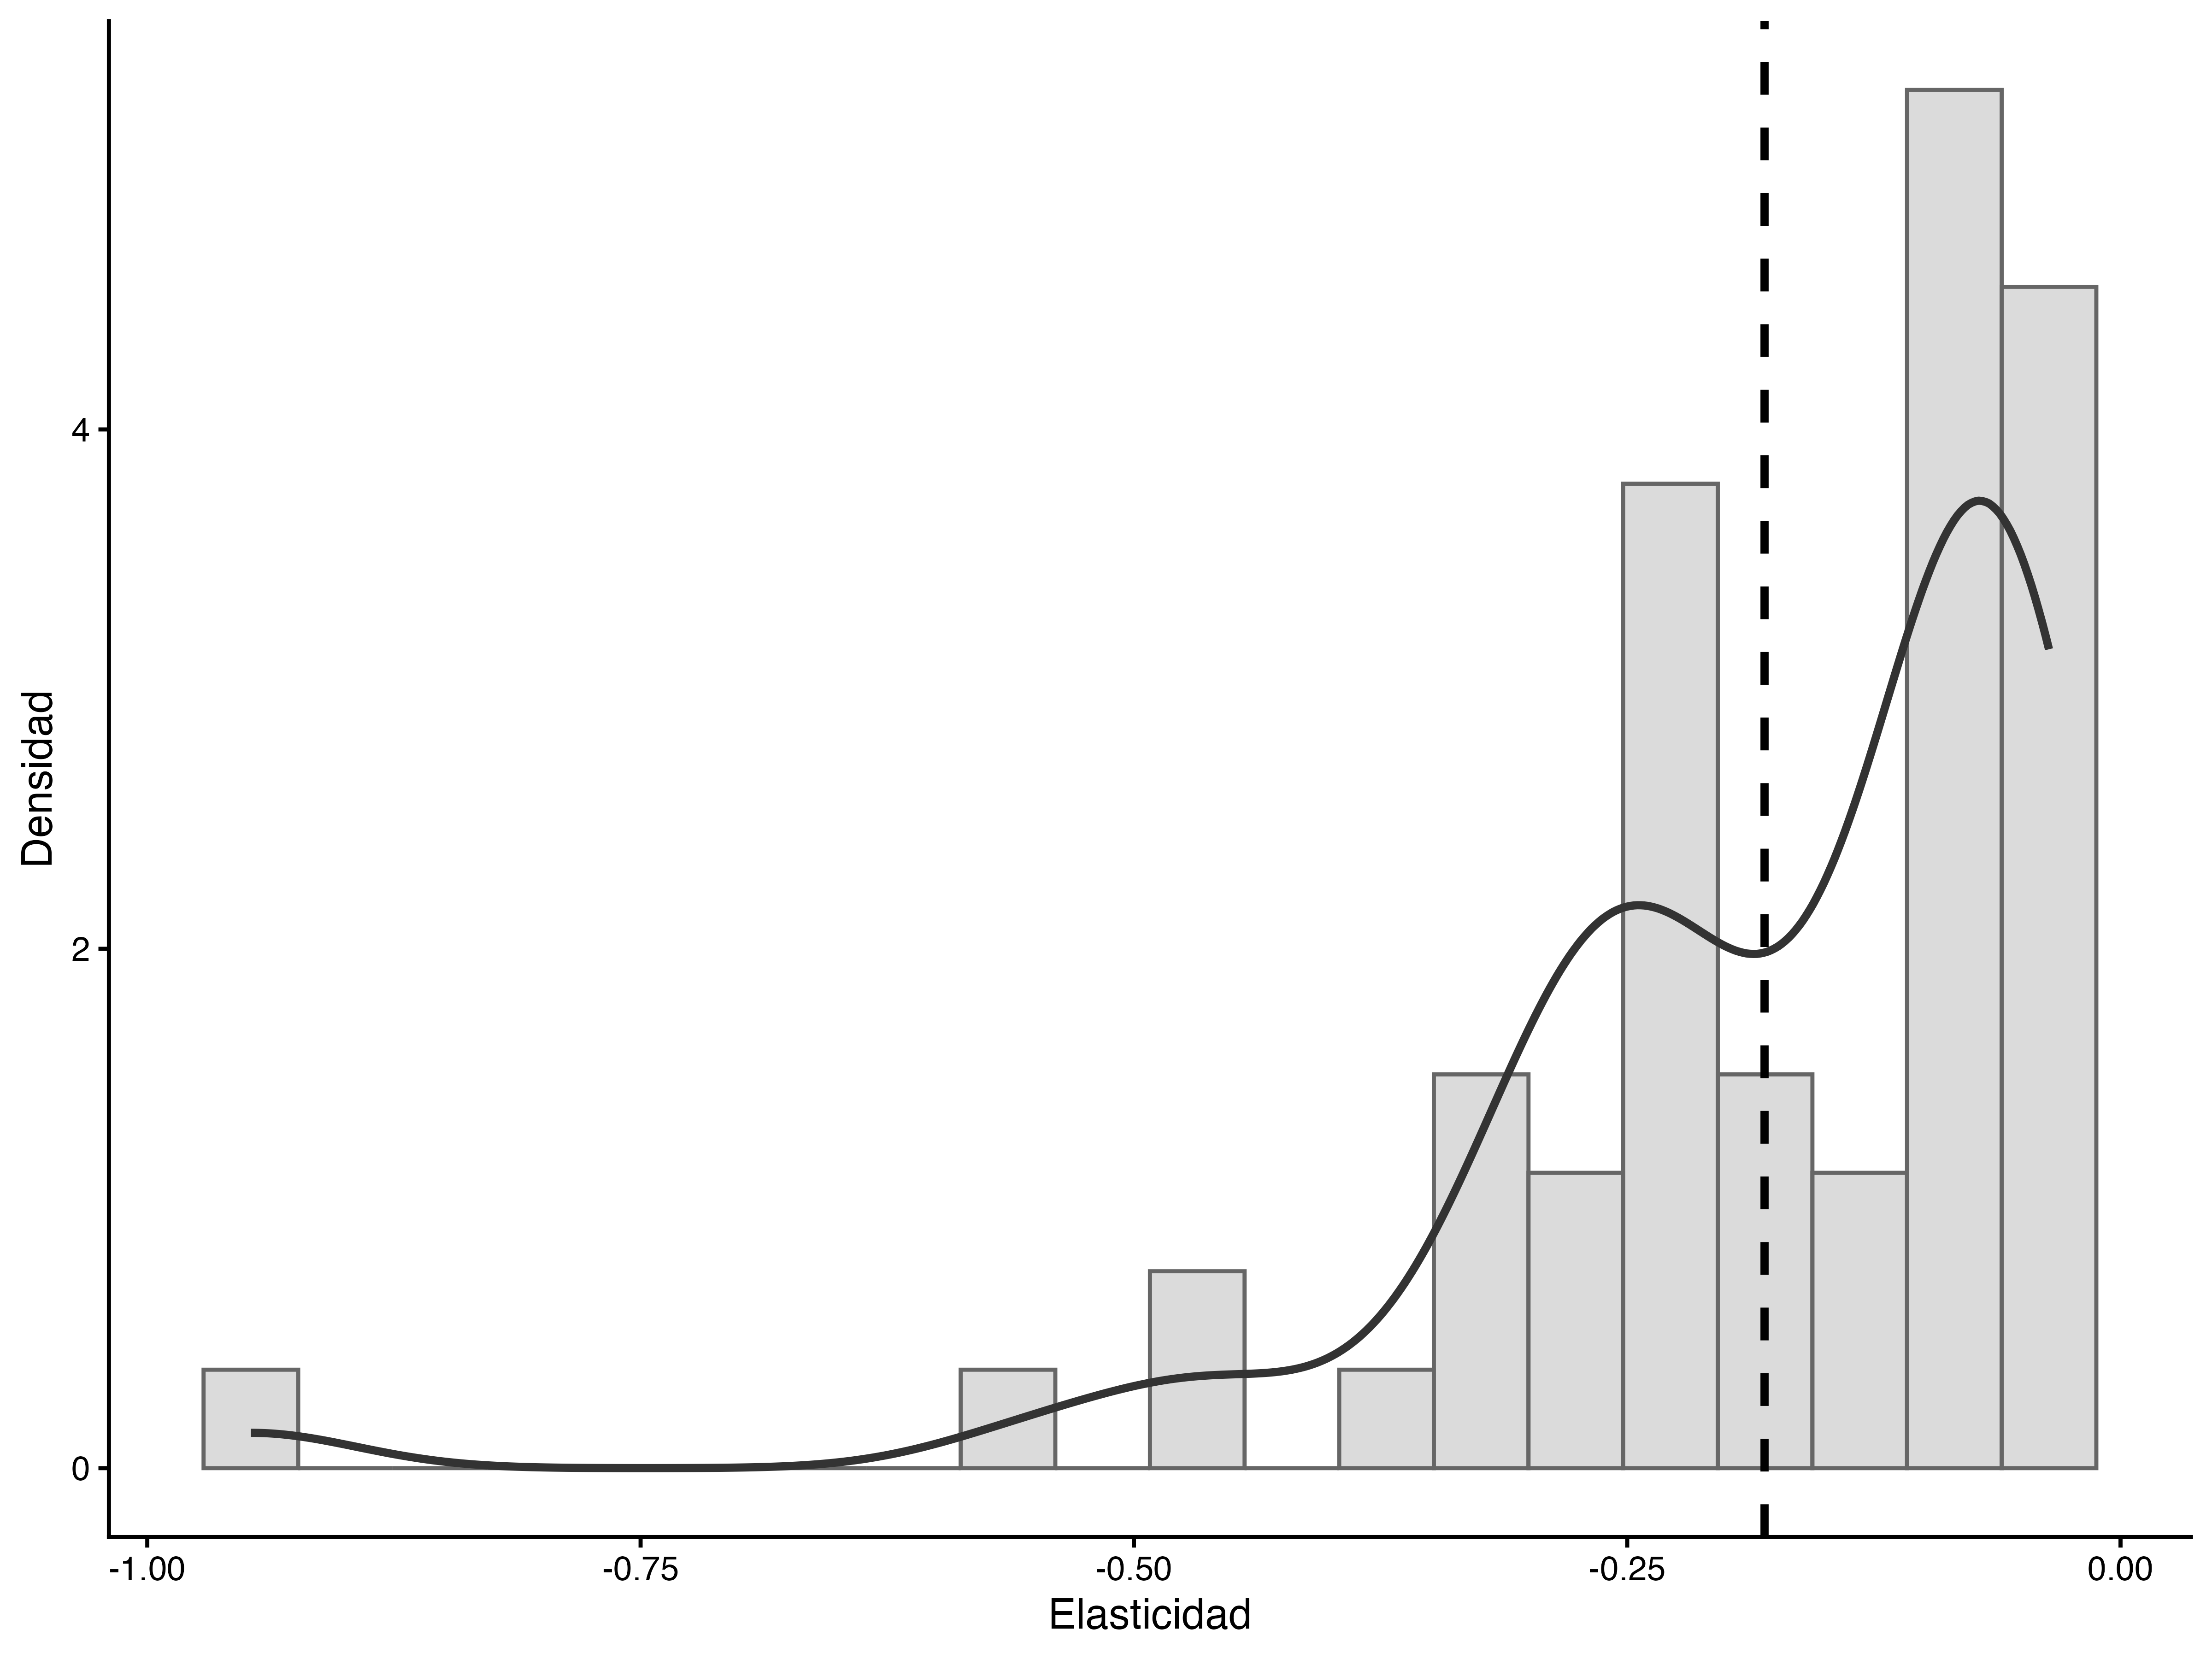
\includegraphics[scale=0.4]{figures/elasticidad_iv3}
    \end{figure}
\end{frame}

\begin{frame}{1. Demanda inelástica y costos heterogéneos}
    \vspace{0.2cm}
\label{frame:est_costs_y}
    \hyperlink{frame:ajuste_modelo}{\beamerbutton{Ajuste del modelo}}
    \scriptsize
\begin{table}[H]
\caption{Estimación de costos marginales}
\label{tab:est_cost}
\centering
\begin{tabular}{lccc}
\hline 
\hline 
Var. Dep.: $C_{i, t}$ (Costos marginales) & (1) & (2) & (3)\\   
\hline 

$T_{t}$ (Tendencia)                   & -9,86$^{***}$ & -8,79$^{***}$ & -11,03 $^{***}$ \\   
                            & (0,8107) & (0,9012) & (0,9364) \\   
$F_{t}$ (Fertilizantes)               & 0,51$^{***}$ & 0,52$^{***}$ & 0,53$^{***}$ \\   
                            & (0,0174) & (0,0191) & (0,0199)\\ 
\textbf{Exposición al calor:} \\
$H_{i, t}$                  & 0,42$^{***}$ & - & 0,36$^{**}$ \\   
                            & (0,1043) & - & (0,1062) \\   
$H_{i, t-1}$                & 0,26$^{*}$ & - & 0,29$^{*}$ \\   
                            & (0,1055) & - & (0,1153)\\ 
\textbf{Exposición al frío:} \\
$C_{i, t}$                  & - & -1,60$^{***}$ & -1,52$^{***}$ \\   
                            & - & (0,3802) & (0,3875)\\   
$C_{i, t-1}$      & - & -0,19 & -0,1486\\   
                            & - & (0,2215) & (0,2355)\\  
\hline
Efecto fijo por país        & $\checkmark$ & $\checkmark$ & $\checkmark$ \\  
\hline
Observaciones               & 1.282 & 1.282 & 1.282\\  
R$^2$                       & 0,2651 & 0,2642 & 0,2713\\  
Within R$^2$                & 0,1404 & 0,1392 & 0,1490\\        
\hline
\hline
\end{tabular}
\end{table}

\end{frame}

\begin{frame}{2. El impacto del estrés térmico}{Construcción de un escenario contrafactual}
    \setbeamertemplate{itemize items}[circle]
    \begin{wideitemize}
        \item <1-> \textbf{Año clave.} En 1989 se acaba el período de cartelización del café. A partir de entonces, los países compiten en virtud de su posición estratégica y condiciones de estrés térmico.
        
        \item <2-> Se construye el promedio de la exposición al estrés térmico observado en 1970-1989, el que se utiliza para estimar los costos marginales contrafactuales en 1990-2019.
        
        \item <3-> Se compara el escenario base (factual) con la construcción sin cambio de tendencia en el estrés térmico (contrafactual). El resultado es el efecto del cambio de tendencia desde 1990 en adelante.
    \end{wideitemize}
    
\end{frame}

\begin{frame}{2. El impacto del estrés térmico}{Resultados agregados}

\scriptsize
\begin{table}[H]
\centering
\caption{Impacto del estrés térmico. Promedio anualizado 1990-2019}
\label{tab:results_1}
\begin{tabular}{lcc}
\hline
\textbf{Escenario} &
\textbf{\begin{tabular}[c]{@{}c@{}}Precio\\ (¢/lb)\end{tabular}} &
\textbf{\begin{tabular}[c]{@{}c@{}}Cantidad\\ (mill. 60 kg.)\end{tabular}} \\ \hline
Sin estrés térmico &
131 &
93,2  \\ 
Con estrés térmico &
138 ($\uparrow$ 5,3\%) &
92,8 ($\downarrow$ 0,5\%) \\
\hline
\end{tabular}%
\end{table}
\scriptsize
\begin{table}[H]
\centering
\caption{Impacto del estrés térmico. Promedio anualizado 1990-2019 (mill. USD)}
\label{tab:results_2}
\begin{tabular}{lcccc}
\hline
\textbf{Escenario} &
  \textbf{\begin{tabular}[c]{@{}c@{}}Excedente\\ líderes \end{tabular}} &
  \textbf{\begin{tabular}[c]{@{}c@{}}Excedente\\ seguidores\end{tabular}} &
  \textbf{\begin{tabular}[c]{@{}c@{}}Excedente\\ importadores\end{tabular}} &
  \textbf{\begin{tabular}[c]{@{}c@{}}Excedente\\ total\end{tabular}} \\ \hline
Sin estrés térmico &
  368  &
  1.689  &
  102.194 &
  104.251  \\ 
Con estrés térmico &
  367 ($\downarrow$ 0,1\%)&
  1.653 ($\downarrow$ 2,2\%) &
  101.240 ($\downarrow$ 0,9\%) &
  103.261 ($\downarrow$ 1\%)  \\
\hline
\end{tabular}
\end{table}

\end{frame}

\begin{frame}{2. El impacto del estrés térmico}{Resultados por país}
    \label{frame:hallazgo2}
    \setbeamertemplate{itemize items}[circle]
    \begin{wideitemize}
        \item <1-> La mayoría de los países exportadores experimentan un incremento en sus costos marginales debido al estrés térmico. \hyperlink{frame:diff_heat_diff_costs}{\beamerbutton{Ver}}
        
        \vspace{0.5cm}
        \item <2-> La reacción de las cantidades, aunque negativas, son acotadas, excepto para los líderes del mercado. \hyperlink{frame:diff_costs_diff_qe}{\beamerbutton{Ver}}
        
        \vspace{0.5cm}
        \item <3-> Los beneficios incorporan también el cambio en precios. Se observan ganadores y perdedores netos. \hyperlink{frame:diff_costs_diff_profit}{\beamerbutton{Ver}}
    \end{wideitemize}
\end{frame}

\begin{frame}{3. Descomposición del efecto total}{Ecuación}
\centering

\[
\Delta\pi = \underbrace{-\Delta c \cdot q^0}_{\substack{\text{Efecto} \\ \text{eficiencia}}} + \underbrace{\Delta P \cdot q^0 + (P^1 - c^1)\Delta q}_{\substack{\text{Efecto} \\ \text{estratégico}}}
\]

\setbeamertemplate{itemize items}[circle]
    \begin{wideitemize}
        \item <1-> \textbf{Efecto eficiencia:} Cambio debido al aumento en costos marginales por estrés térmico, manteniendo fija la estructura estratégica del mercado.

        \item <2-> \textbf{Efecto estratégico:} Cambio en cantidades y precios debido a la reconfiguración del equilibrio estratégico del mercado.
    \end{wideitemize}  

\end{frame}
\begin{frame}{3. Descomposición del efecto total}{Resultados}
    \label{frame:descomposicion1}
    \setbeamertemplate{itemize items}[circle]
    \begin{wideitemize}
        \item A nivel agregado, el efecto eficiencia domina las pérdidas totales. El efecto estratégico las mitiga parcialmente.
        
            \vspace{0.3cm}
            \scriptsize
\begin{table}[H]
\centering
\caption{Descomposición de la pérdida de excedente. Total 1990-2019 (mill. USD)}
\label{tab:descomp_g}
\begin{tabular}{lccc}
\hline
            & \textbf{Efecto eficiencia} & \textbf{Efecto estratégico} & \textbf{Efecto total} \\ \hline
Líderes     & 10.723 (50\%)             & -10.710 (50\%)            & 13          \\
Seguidores  & 12.867 (53\%)             & -11.621 (47\%)            & 1.246       \\ \hline
\end{tabular}%

\end{table}
            \vspace{0.3cm}
        \item El resultado neto se define por la magnitud relativa de ambos efectos. \hyperlink{frame:efecto_estrategico1}{\beamerbutton{Efecto estratégico y pérdida total}}
    \end{wideitemize}
\end{frame}

\section{Conclusiones}
\begin{frame}{Conclusiones}
    \setbeamertemplate{itemize items}[circle]
    \begin{wideitemize}
        \item <1-> El estrés térmico incrementa los costos marginales de producción, \pause \textbf{\color{amaranth} pero los agentes responden estratégicamente, mitigando parcialmente las pérdidas totales.}

        \item <2-> Modelos reducidos podrían sobreestimar las pérdidas totales al no considerar la reconfiguración del equilibrio estratégico.

        \item <3-> Se agudizan las asimetrías iniciales. A nivel agregado, los seguidores se ven más afectados por el estrés térmico. Los líderes neutralizan el impacto.
        
        \item <4-> El efecto neto depende de la magnitud relativa del efecto eficiencia y el efecto estratégico. Este último varía con la elasticidad de la demanda y el cambio en costos marginales.

    \end{wideitemize}
\end{frame}

\setbeamertemplate{footline}{} 
\setcounter{framenumber}{0} 
\section*{Apéndices}

\begin{frame}{Apéndice}{Oligopolio jerárquico \hyperlink{frame:mercado_supuestos}{\beamerbutton{Volver}}
}
    \label{frame:oligopolio_plot}
    \begin{figure}[H]
    \centering
    \begin{minipage}[t]{0.45\textwidth}
        \centering
        \caption{Participación de mercado de líderes}
        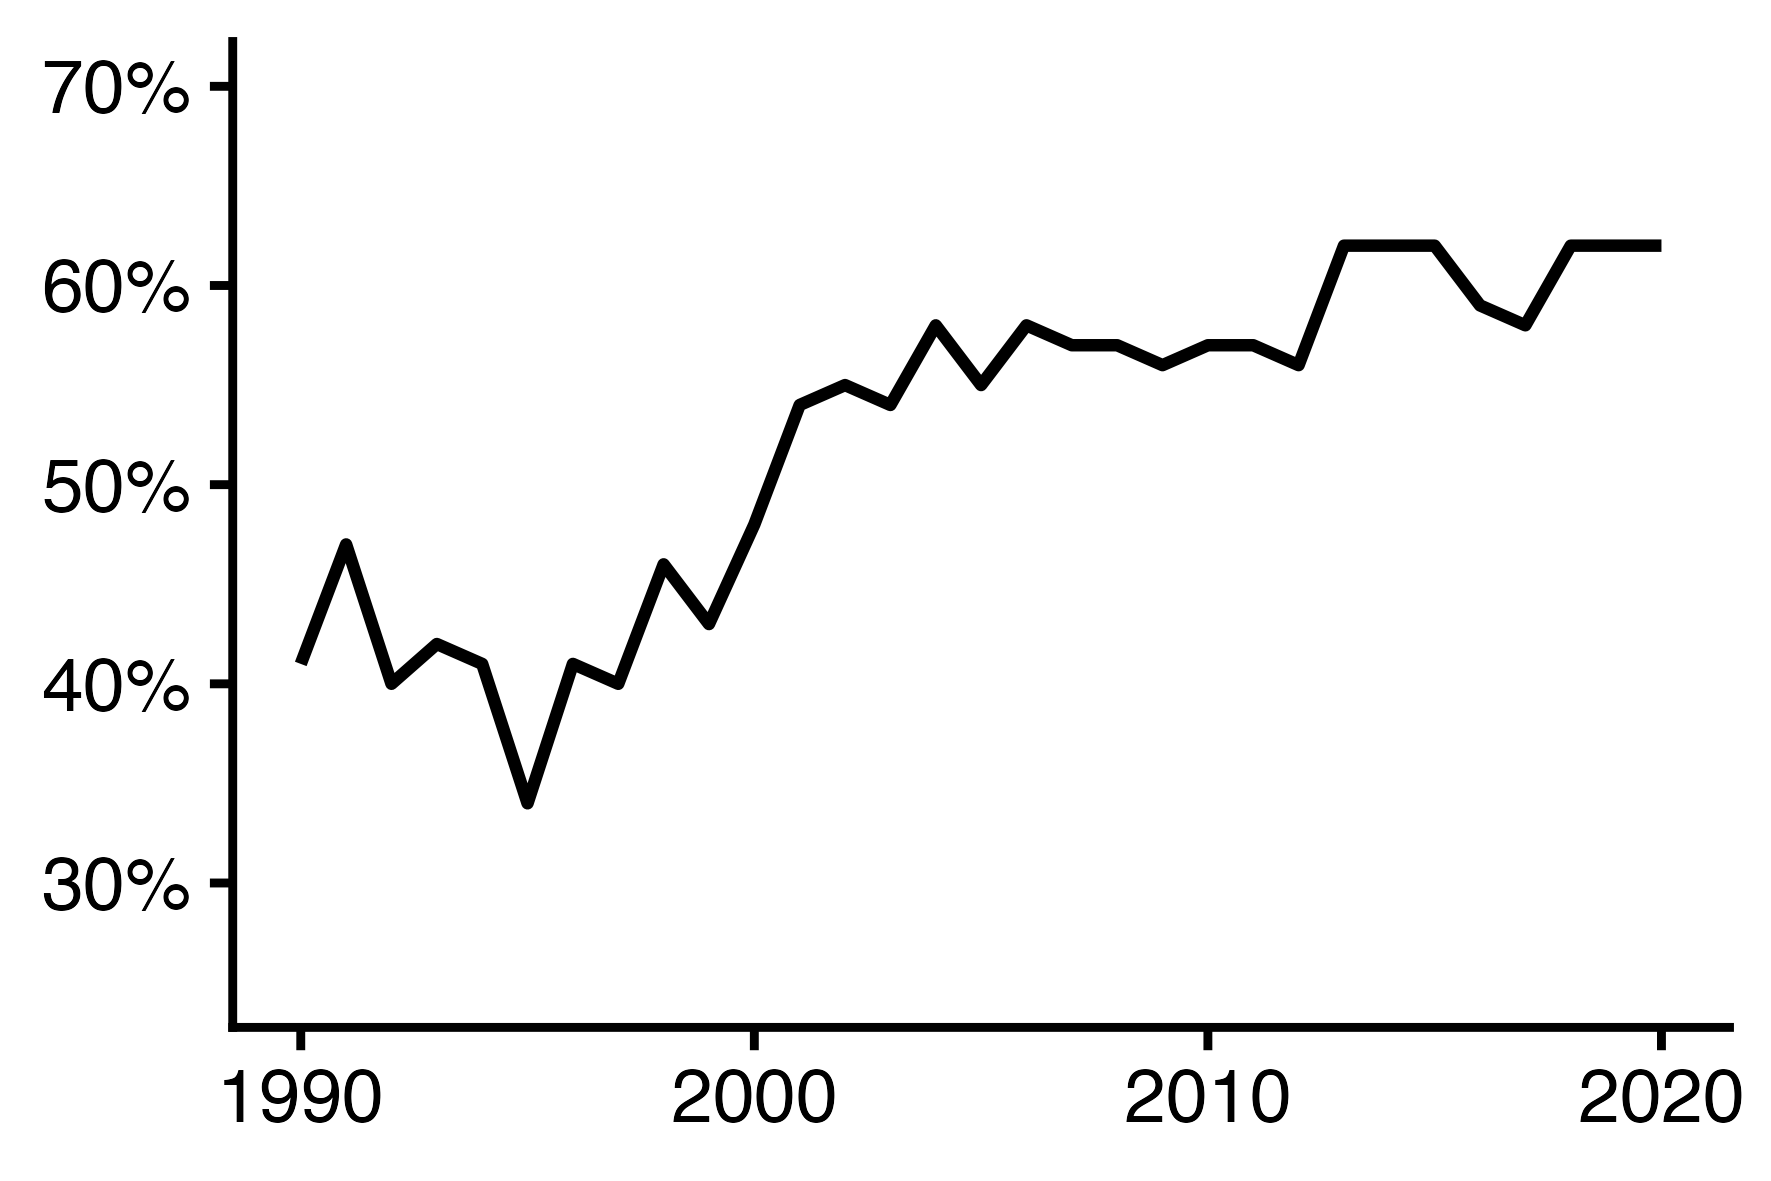
\includegraphics[width=\linewidth]{figures/c3}
        \label{fig:c3}
    \end{minipage}
    \hfill
    \begin{minipage}[t]{0.45\textwidth}
        \centering
        \caption{Cantidades por grupo exportador}
        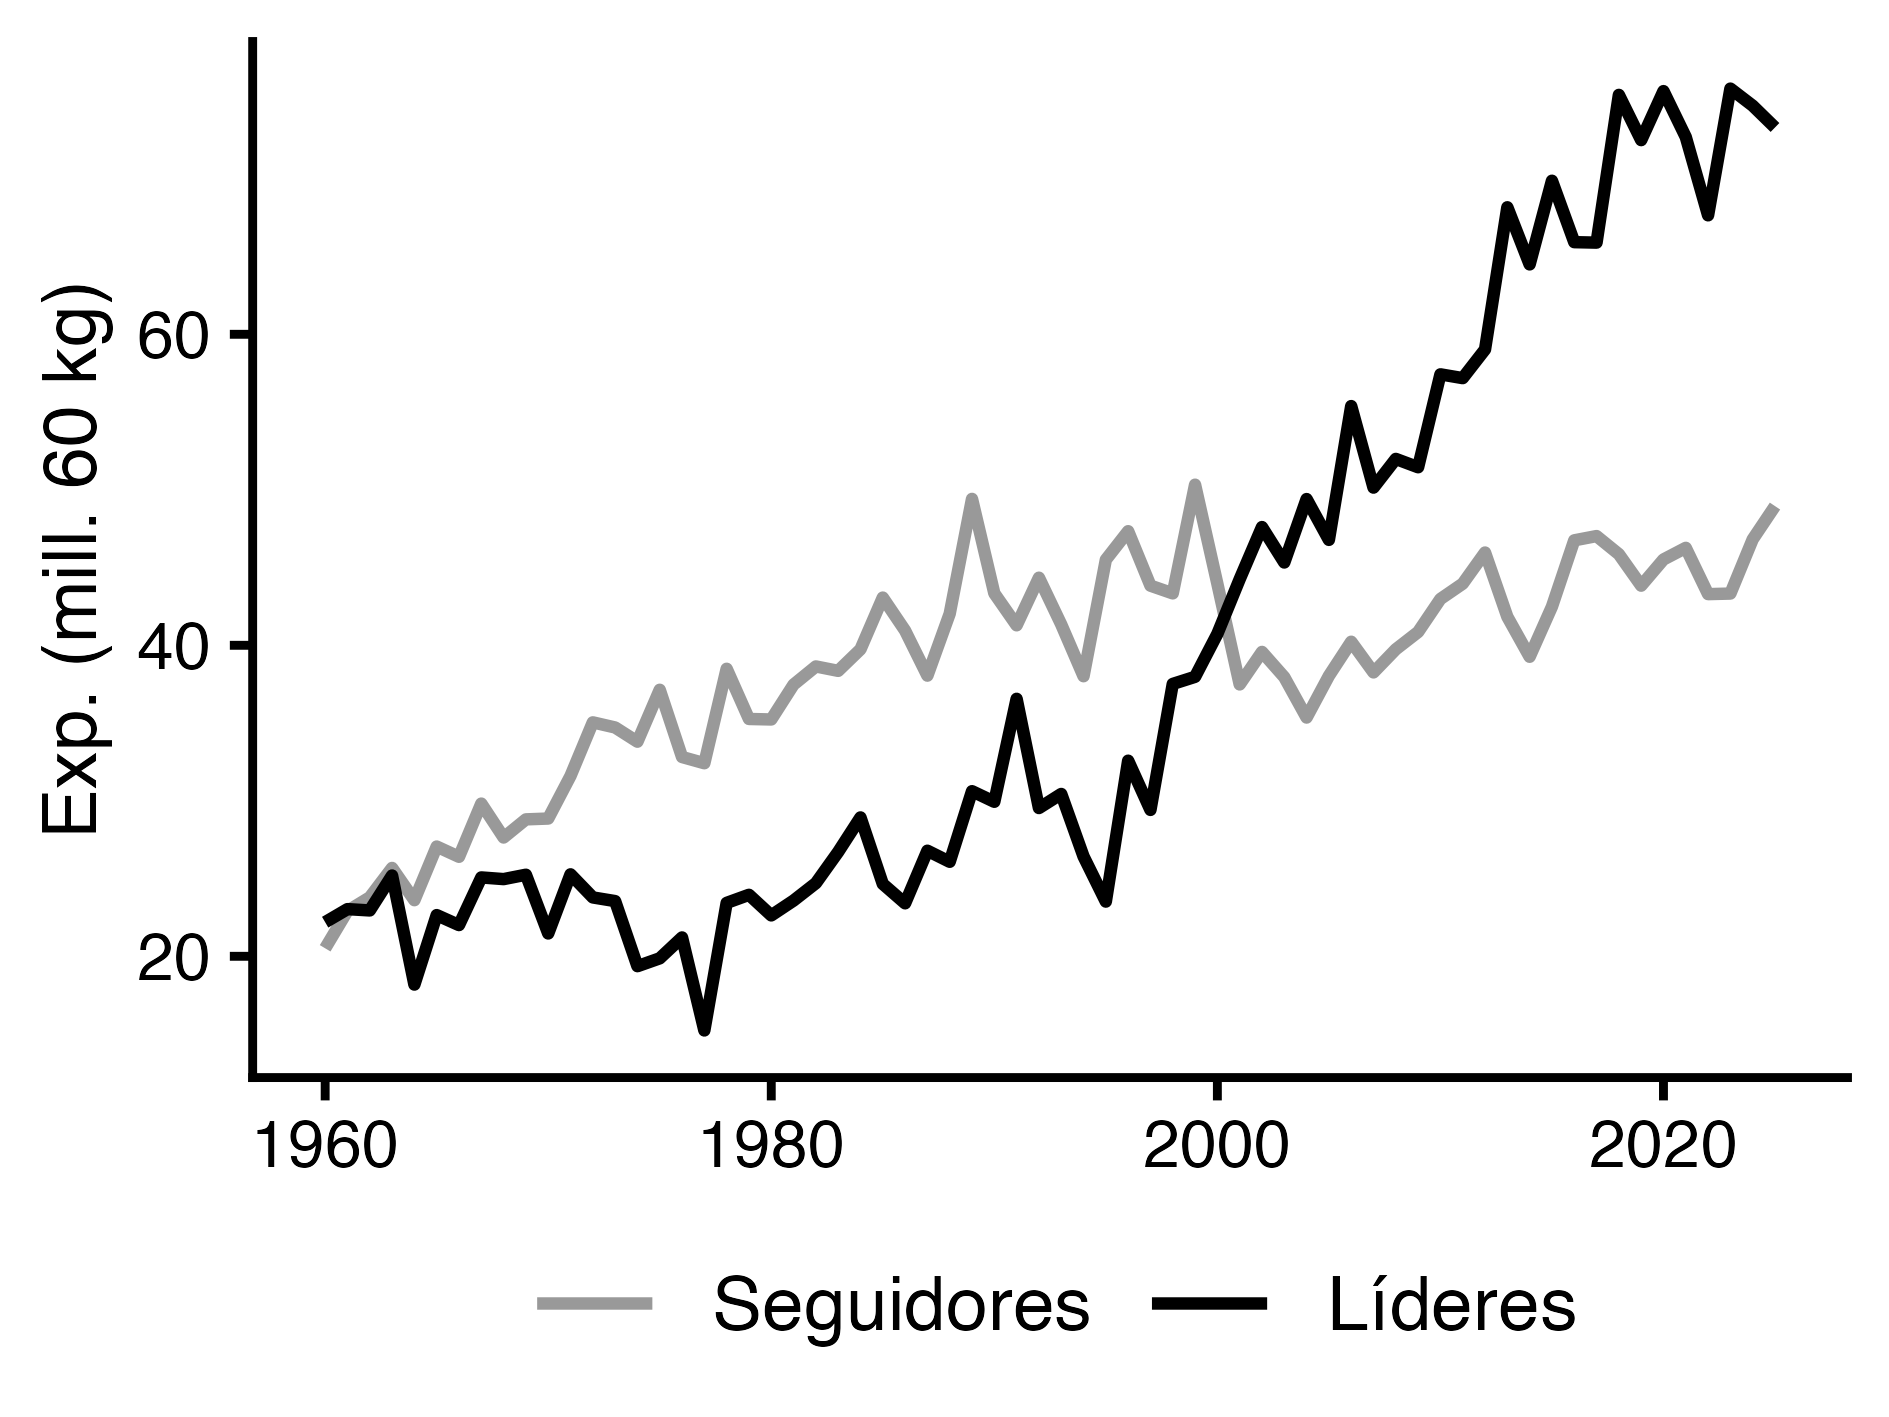
\includegraphics[width=\linewidth]{figures/leaders}
        \label{fig:leaders}
    \end{minipage}
\end{figure}
\end{frame}

\begin{frame}{Apéndice}{Sensibilidad al estrés térmico \hyperlink{frame:mercado_supuestos}{\beamerbutton{Volver}}} 
    \label{frame:estres_plot}
    \scriptsize
\begin{table}[H]
\centering
\caption{Efecto de la temperatura en los países productores}
\label{tab:motiv}
\begin{tabular}{lccc}
\hline
\hline

& \textbf{Cantidad} & \textbf{Ingresos} & \textbf{Participación} \\
& \textbf{(log)} & \textbf{(log)} & \textbf{de mercado} \\
& (1) & (2) & (3) \\
\midrule
Temperatura & 0.343*** & 1.015*** & 1.618*** \\
& (0.0265) & (0.0760) & (0.173) \\
Temperatura$^2$ & -0.00898*** & -0.0274*** & -0.0424*** \\
& (0.000639) & (0.00184) & (0.00418) \\
Constante & -2.404*** & -4.309*** & -11.99*** \\
& (0.275) & (0.788) & (1.796) \\
\midrule
Observaciones & 2,532 & 2,532 & 2,532 \\
R$^2$ aj. & 0.0826 & 0.105 & 0.0446 \\
\hline
\hline
\end{tabular}
\end{table}

\end{frame}

\begin{frame}{Apéndice}{Sensibilidad al estrés térmico \hyperlink{frame:mercado_supuestos}{\beamerbutton{Volver}}
} 
    \begin{figure}[H]
    \centering
    \begin{minipage}[t]{0.45\textwidth}
        \centering
        \caption{Temperatura y cantidades}
        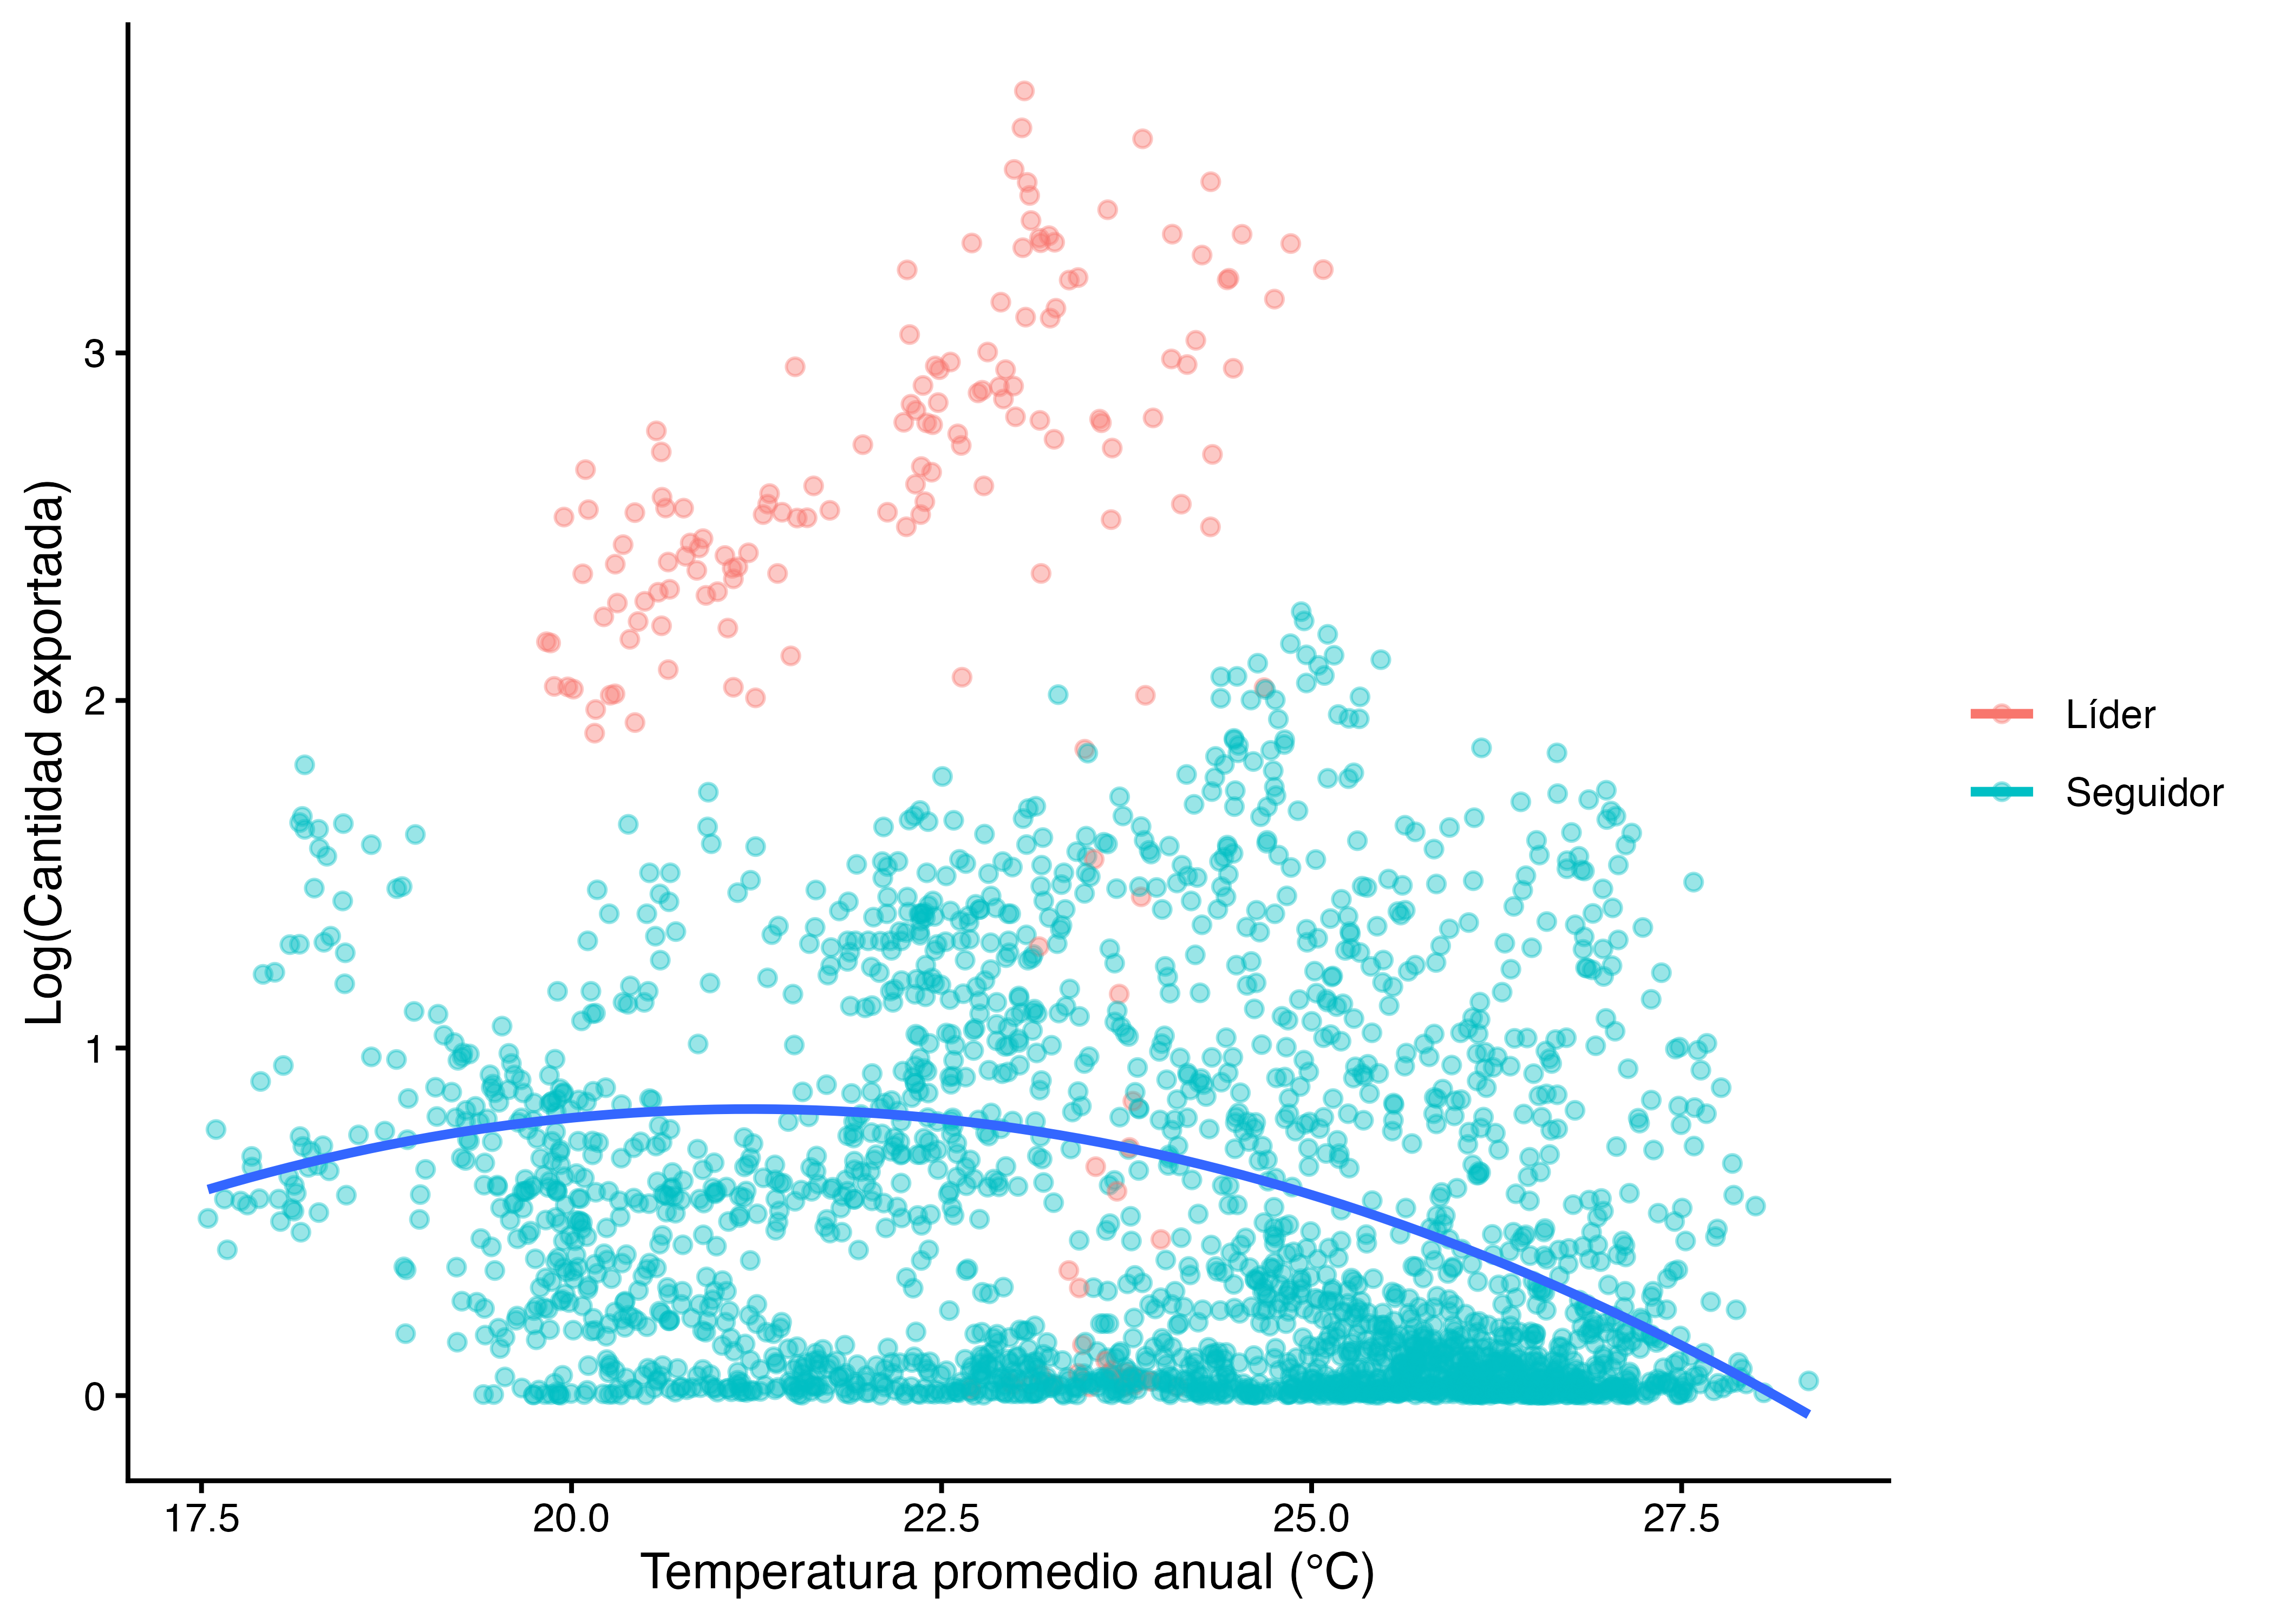
\includegraphics[width=\linewidth]{figures/motiv1}
        \label{fig:estres_qe}
    \end{minipage}
    \hfill
    \begin{minipage}[t]{0.45\textwidth}
        \centering
        \caption{Temperatura e ingresos}
        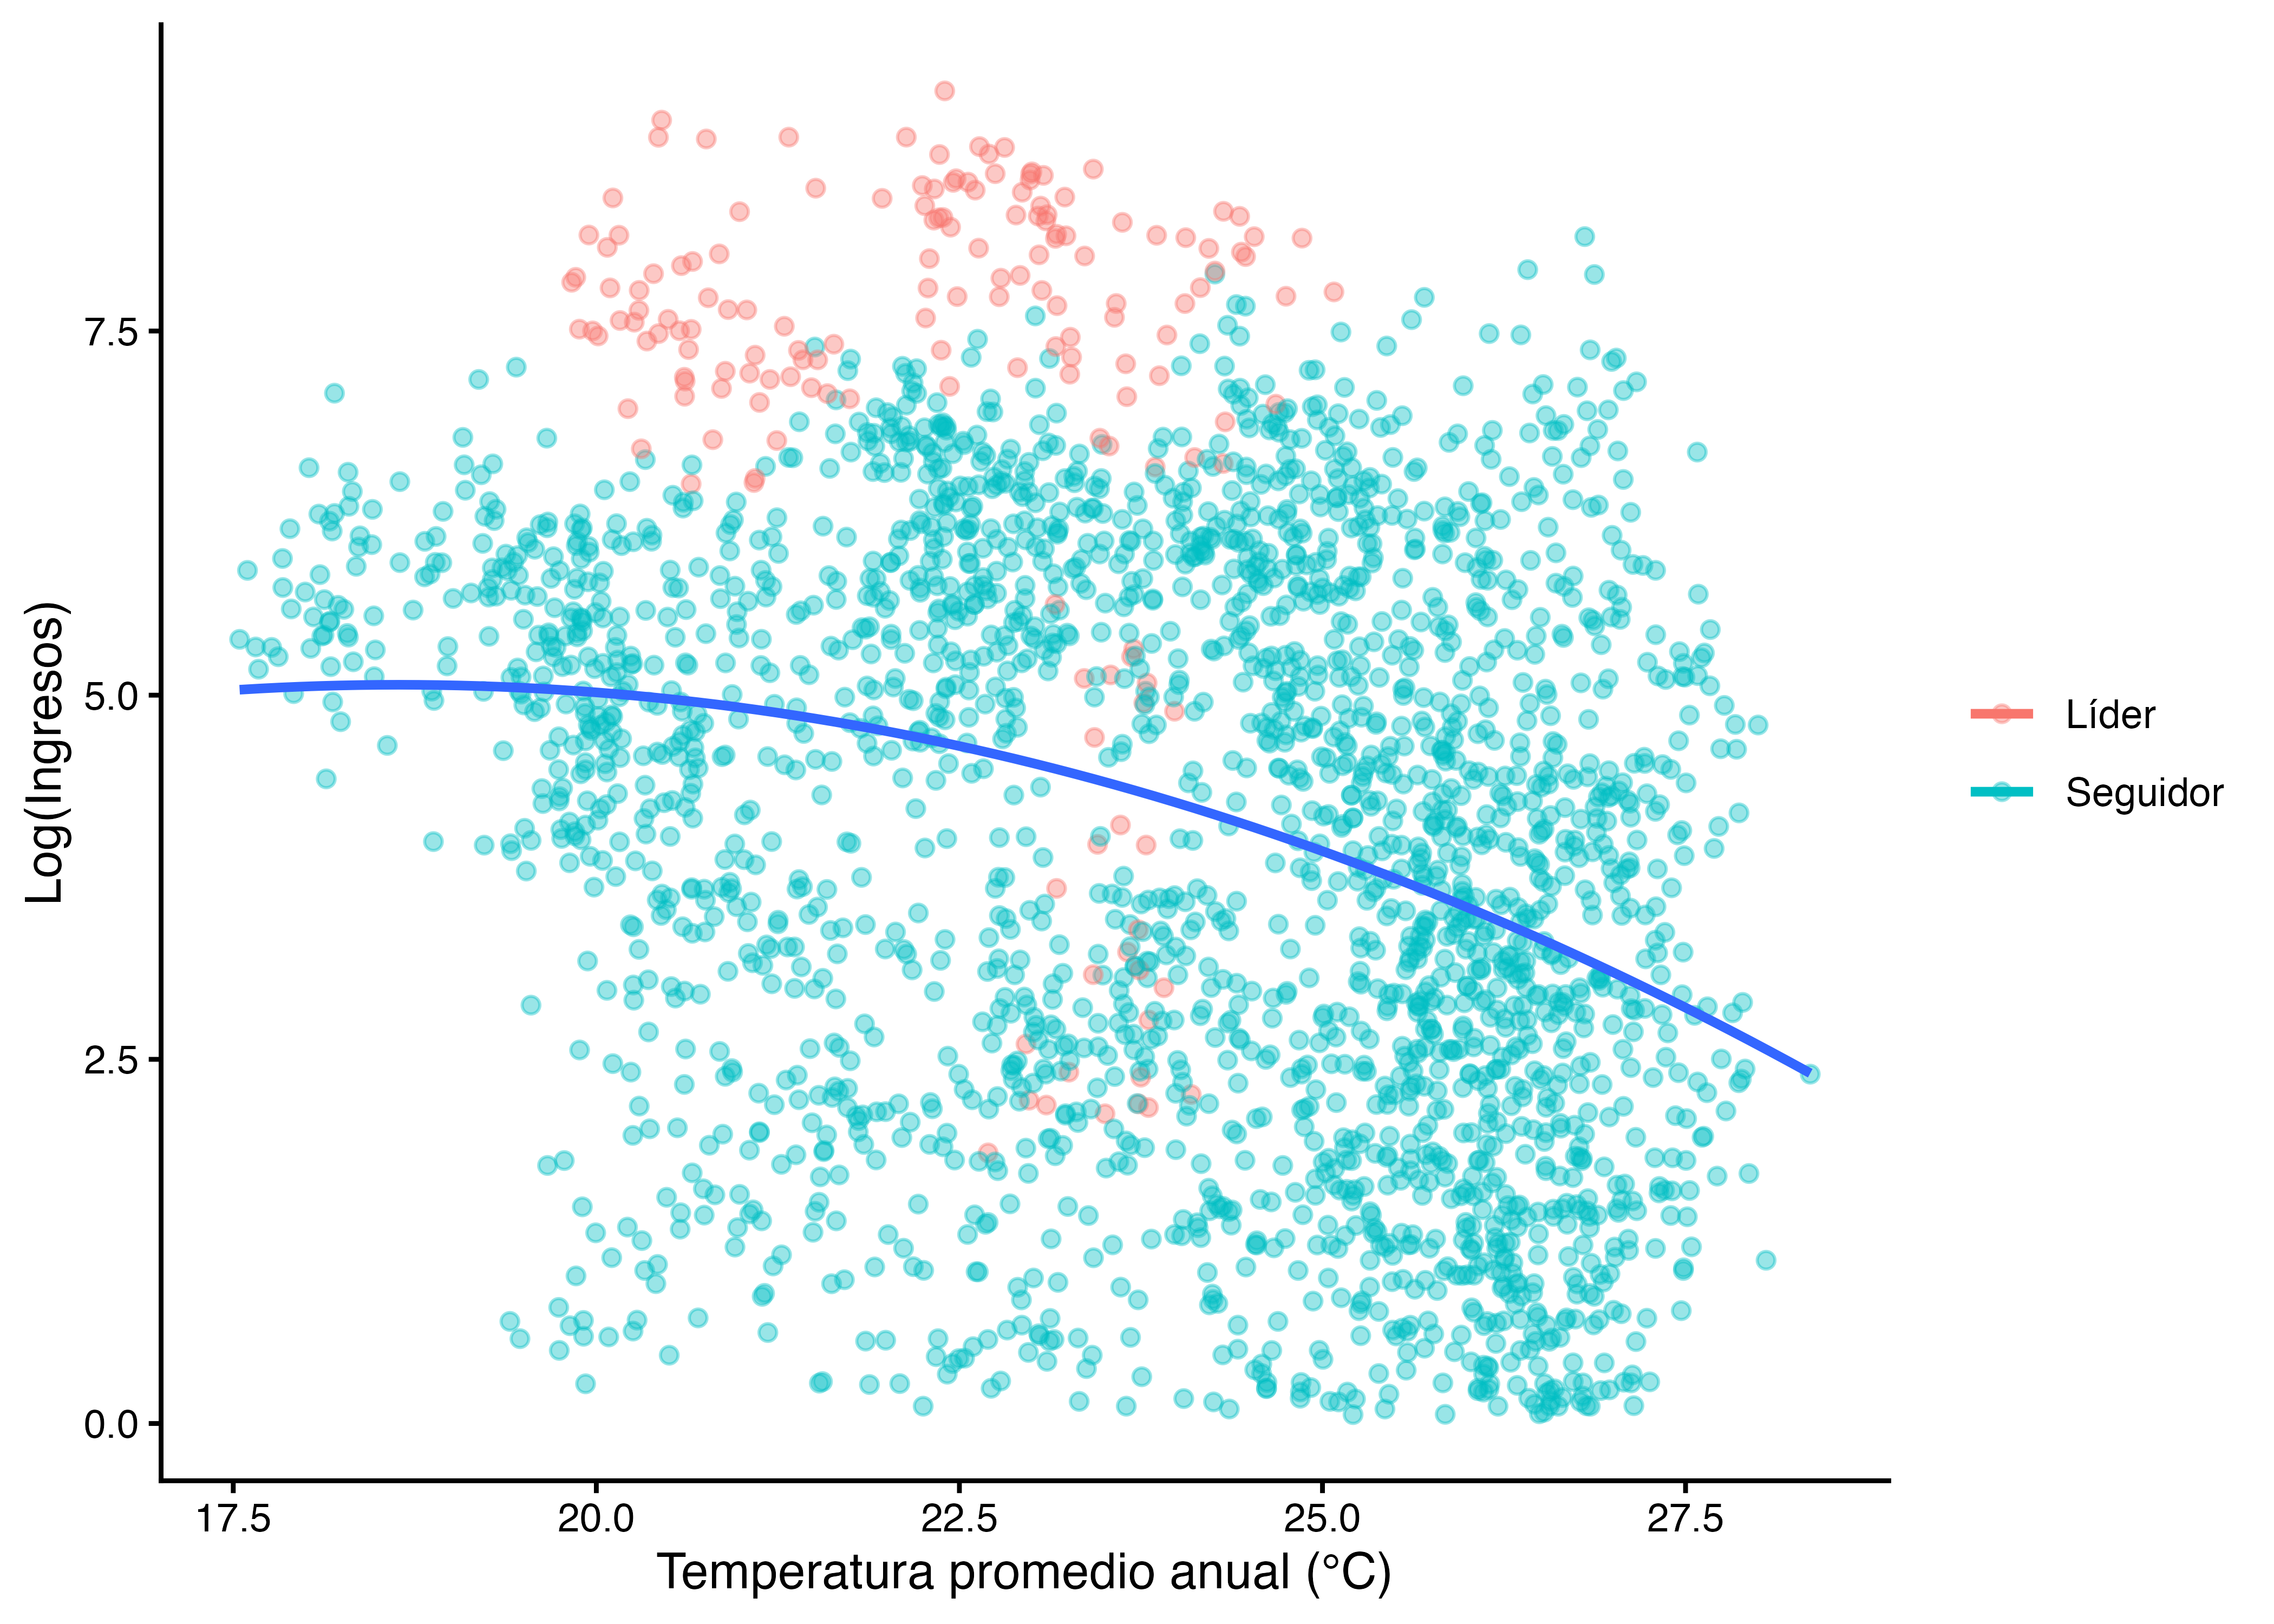
\includegraphics[width=\linewidth]{figures/motiv2}
        \label{fig:estres_rev}
    \end{minipage}
\end{figure}
\end{frame}

\begin{frame}{Apéndice}{Sensibilidad al estrés térmico \hyperlink{frame:mercado_supuestos}{\beamerbutton{Volver}}} 
    
    \begin{figure}[H]
    \centering      
    \caption{Temperatura y participación de mercado}
    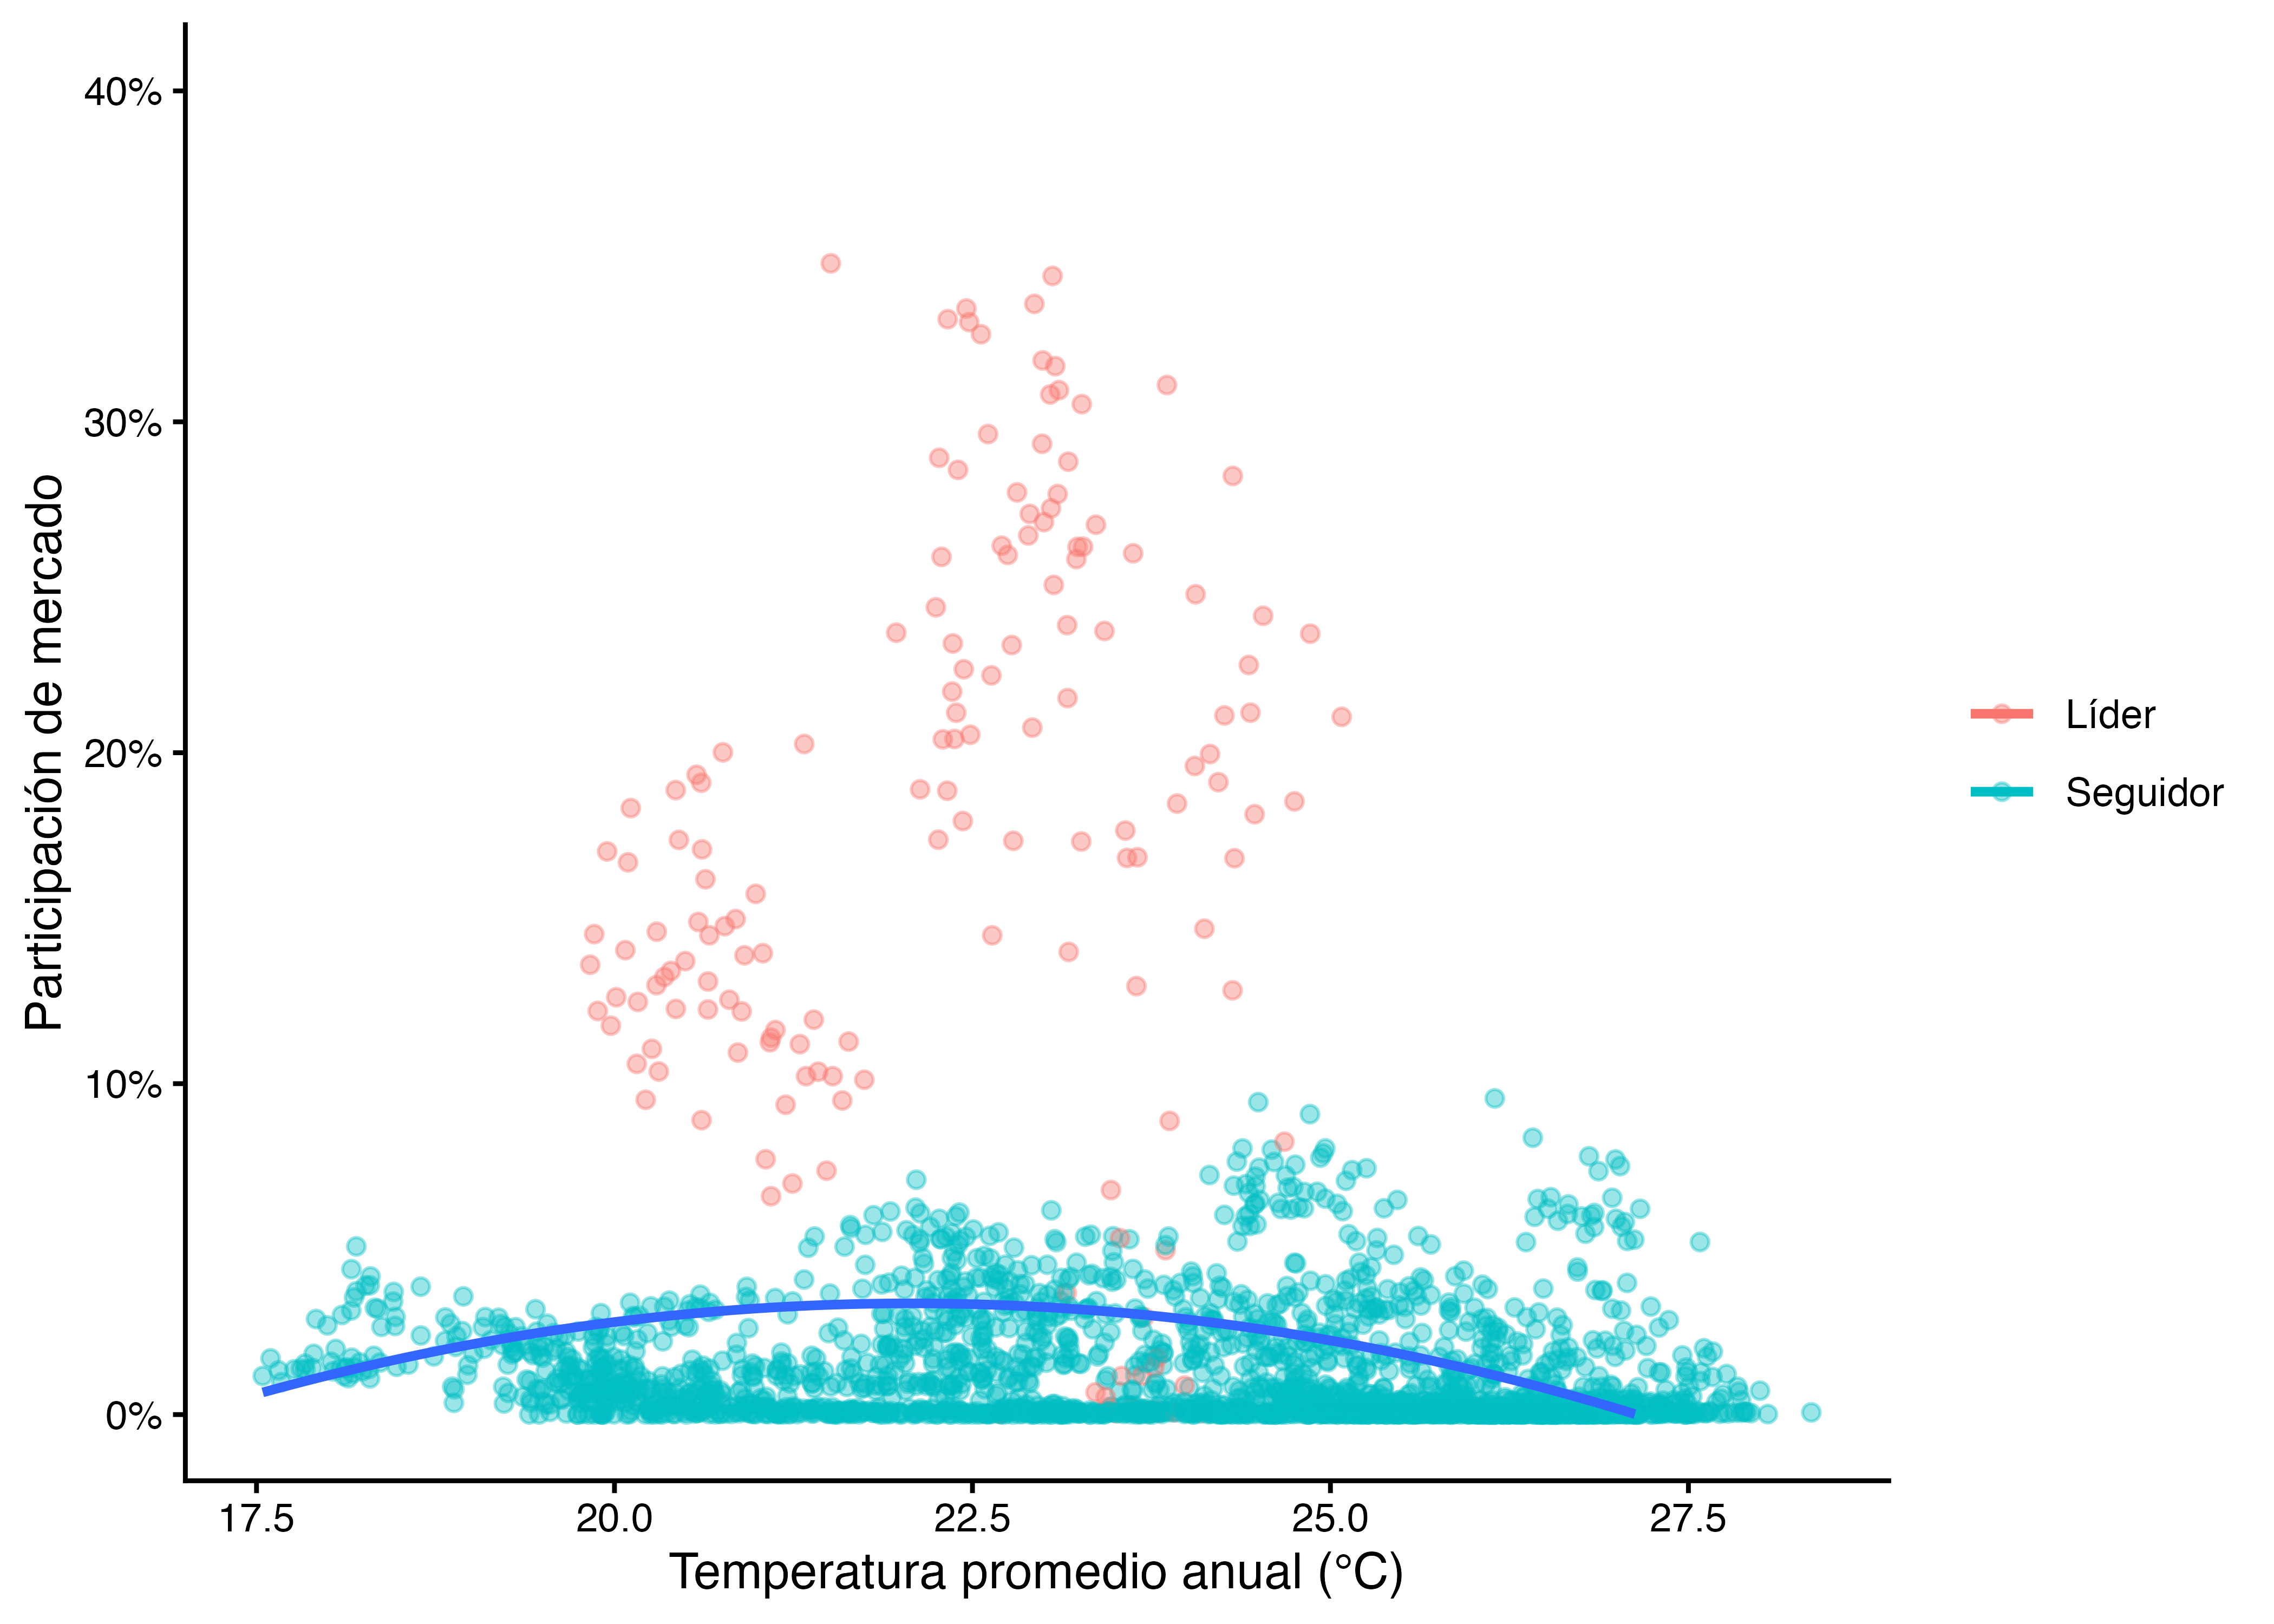
\includegraphics[scale=0.5]{figures/motiv3}
    \end{figure}
\end{frame}
\begin{frame}{Apéndice}{Variable de estrés térmico \hyperlink{frame:datos}{\beamerbutton{Volver}}}
    \label{frame:variable_estres}
    \setbeamertemplate{itemize items}[circle]
    \begin{wideitemize}
        \item Se considera que la temperatura sigue una trayectoria triangular en el día, con un máximo $T_{max}$ y un mínimo $T_{min}$.
        \item Esto permite calcular la fracción del día en que la temperatura excede un umbral $T_{umbral}$.
        \item Umbrales diferentes por especie (30°C Robusta, 26°C Arábica).
        \item Ponderación por hectáreas cultivadas en 2020.
    \end{wideitemize}

\end{frame}

\begin{frame}{Apéndice}{Variable de estrés térmico \hyperlink{frame:datos}{\beamerbutton{Volver}}}
    \begin{figure}[H]
    \centering
    \begin{minipage}[t]{0.45\textwidth}
        \centering
        \caption{Exposición total al frío}
        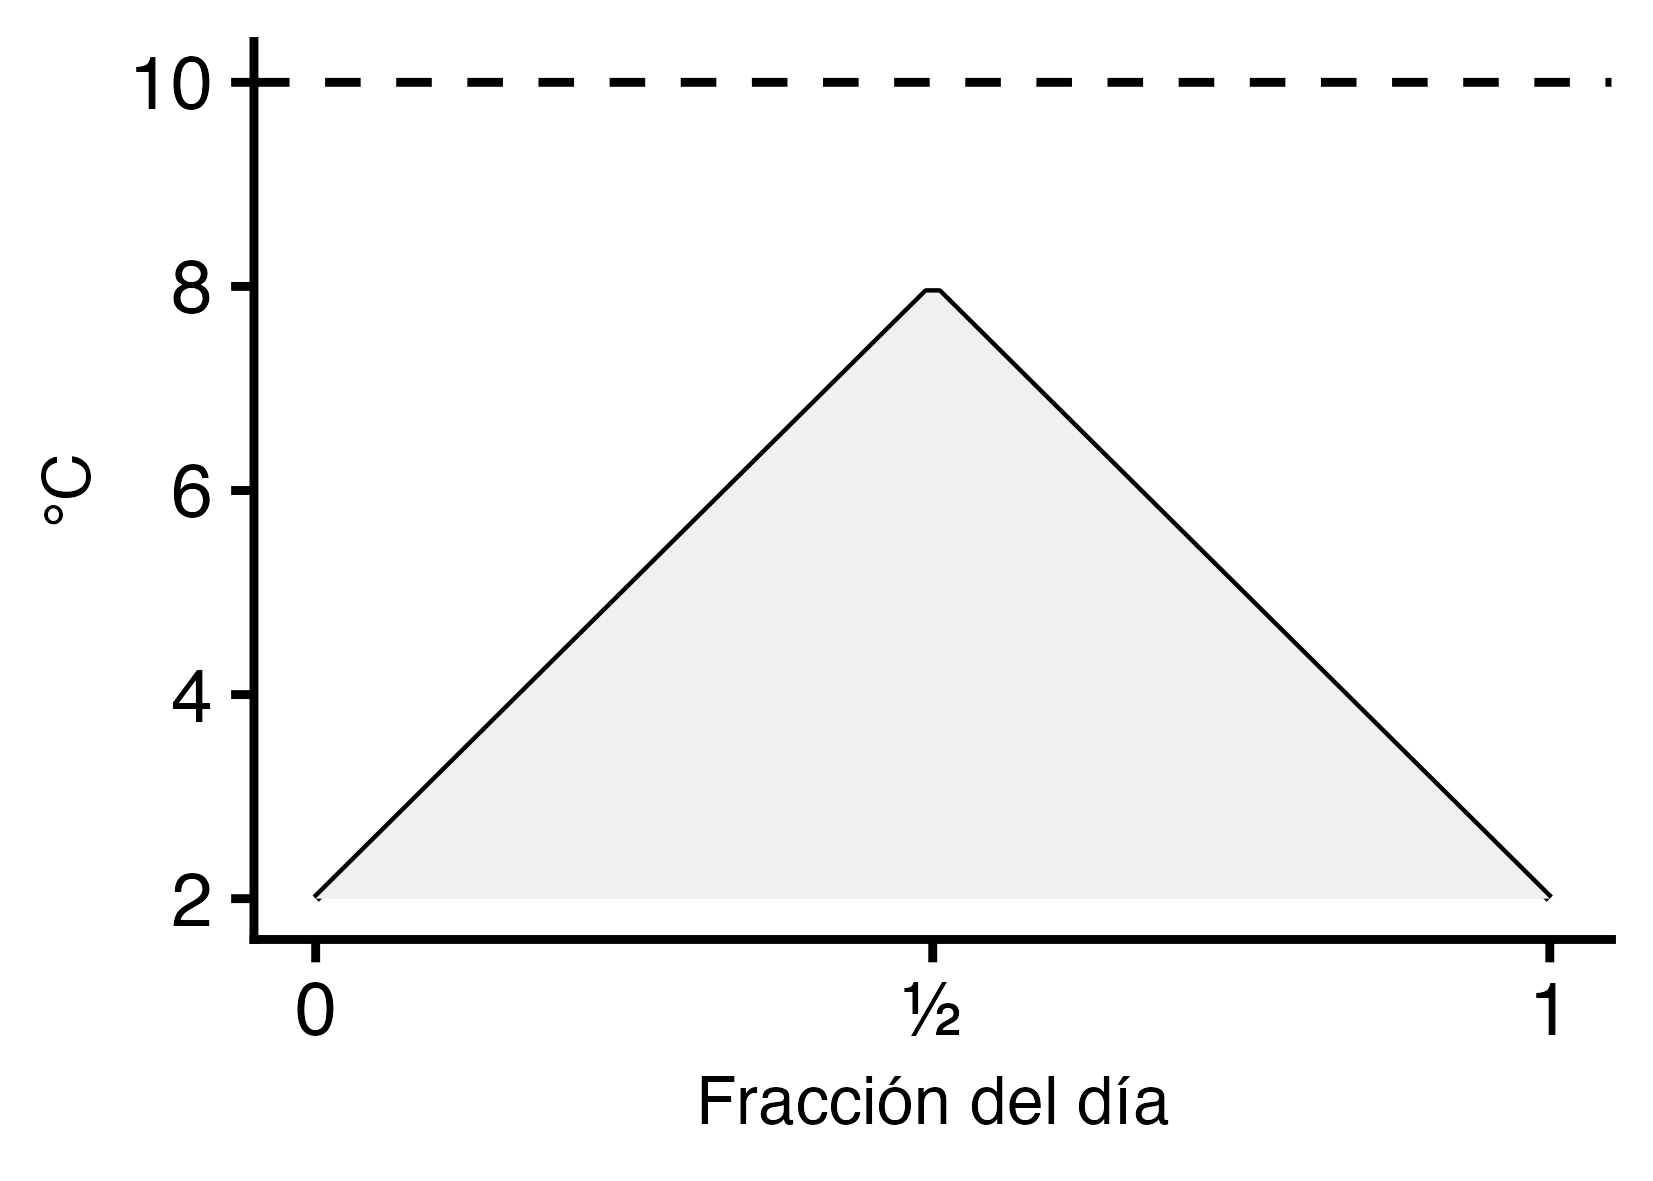
\includegraphics[width=\linewidth]{figures/exp_p1}
        \label{fig:exp_p1}
    \end{minipage}
    \hfill
    \begin{minipage}[t]{0.45\textwidth}
        \centering
        \caption{Sin exposición al calor}
        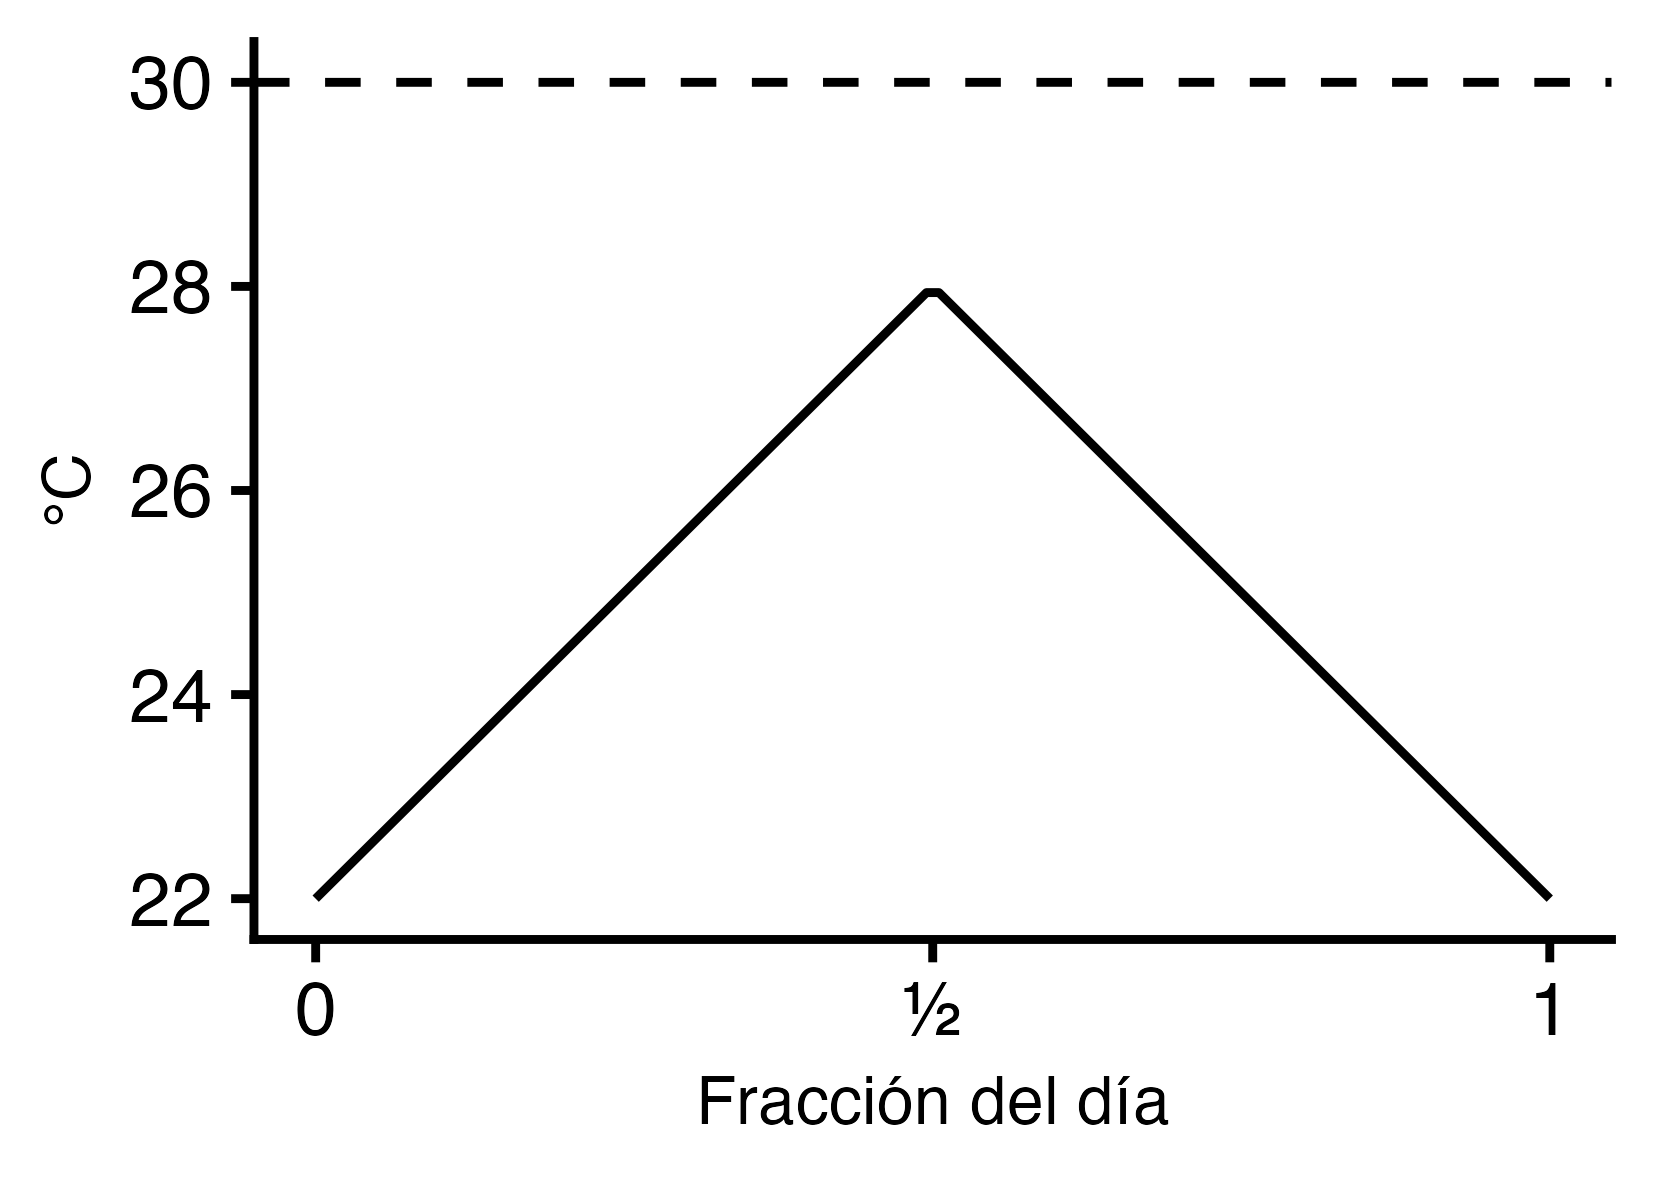
\includegraphics[width=\linewidth]{figures/exp_p4}
        \label{fig:exp_p4}
    \end{minipage}
\end{figure}
\end{frame}

\begin{frame}{Apéndice}{Variable de estrés térmico \hyperlink{frame:datos}{\beamerbutton{Volver}}}
\begin{figure}[H]
    \centering
    \begin{minipage}[t]{0.45\textwidth}
        \centering
        \caption{Exposición parcial al frío}
        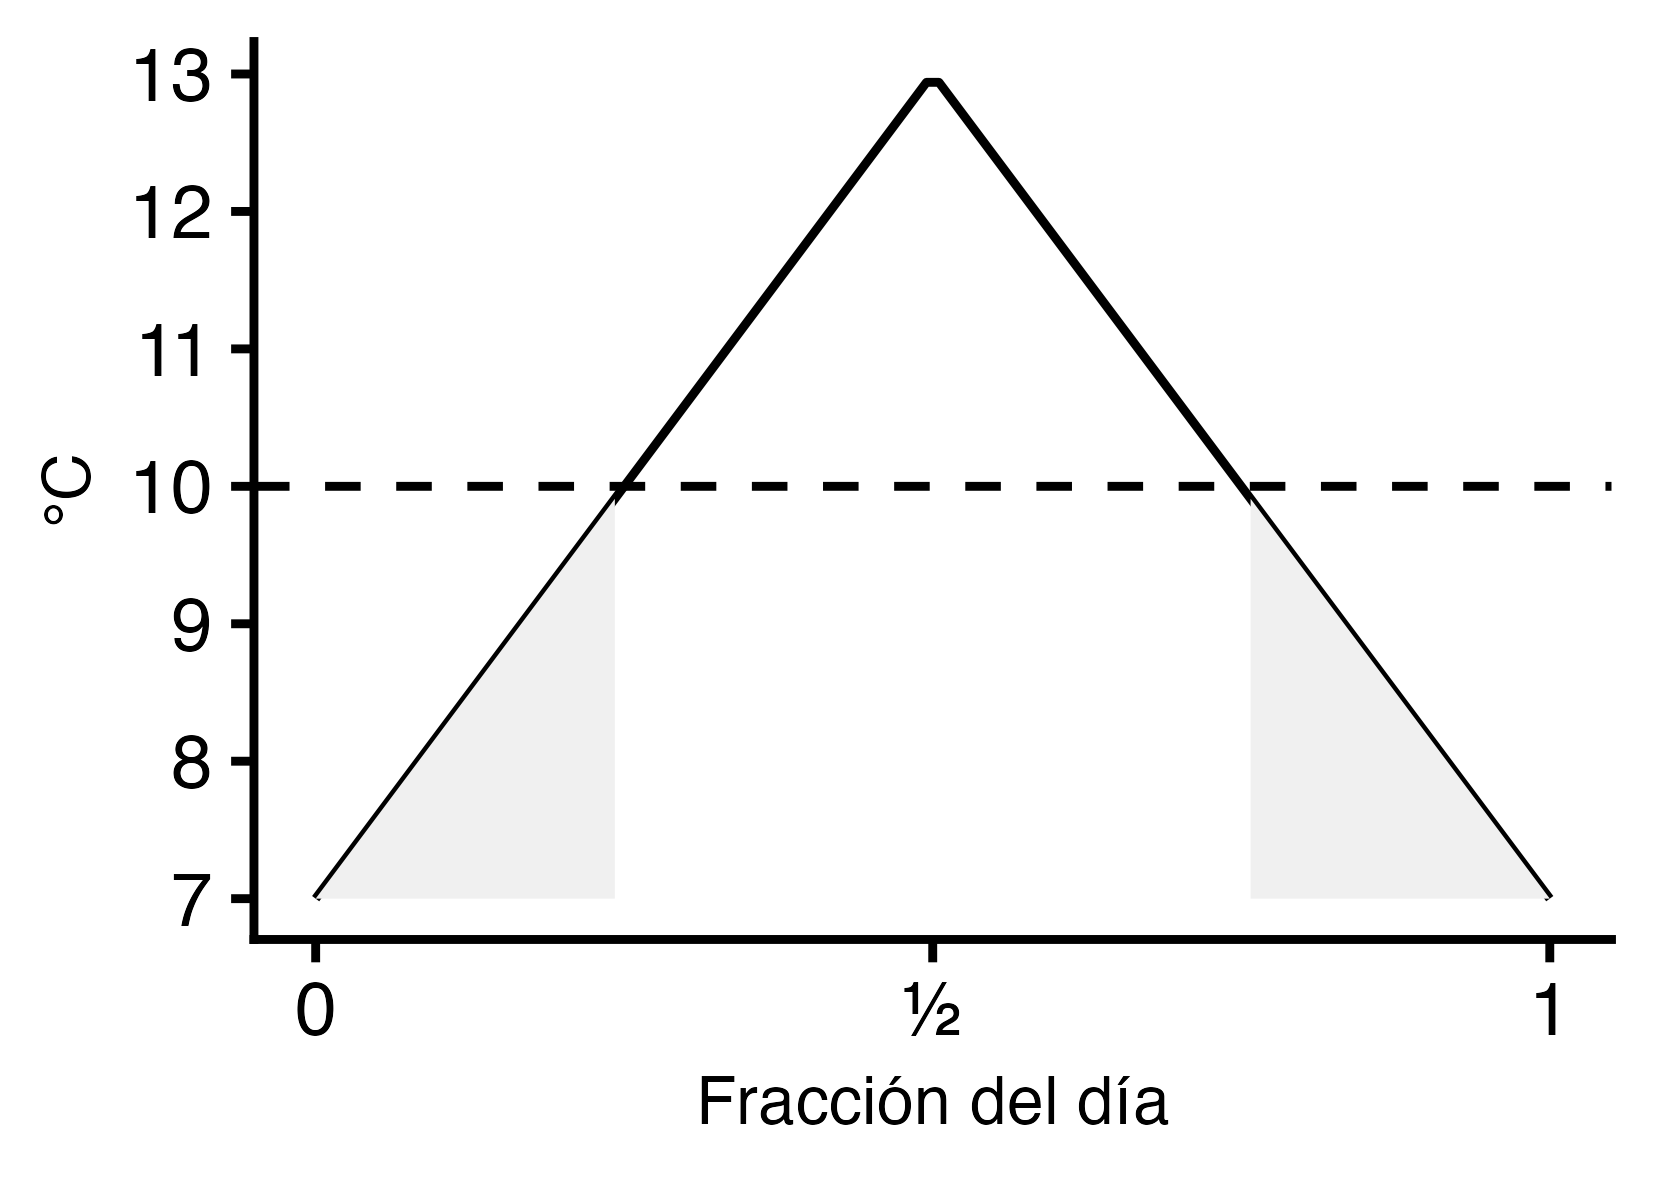
\includegraphics[width=\linewidth]{figures/exp_p2}
        \label{fig:exp_p2}
    \end{minipage}
    \hfill
    \begin{minipage}[t]{0.45\textwidth}
        \centering
        \caption{Exposición parcial al calor}
        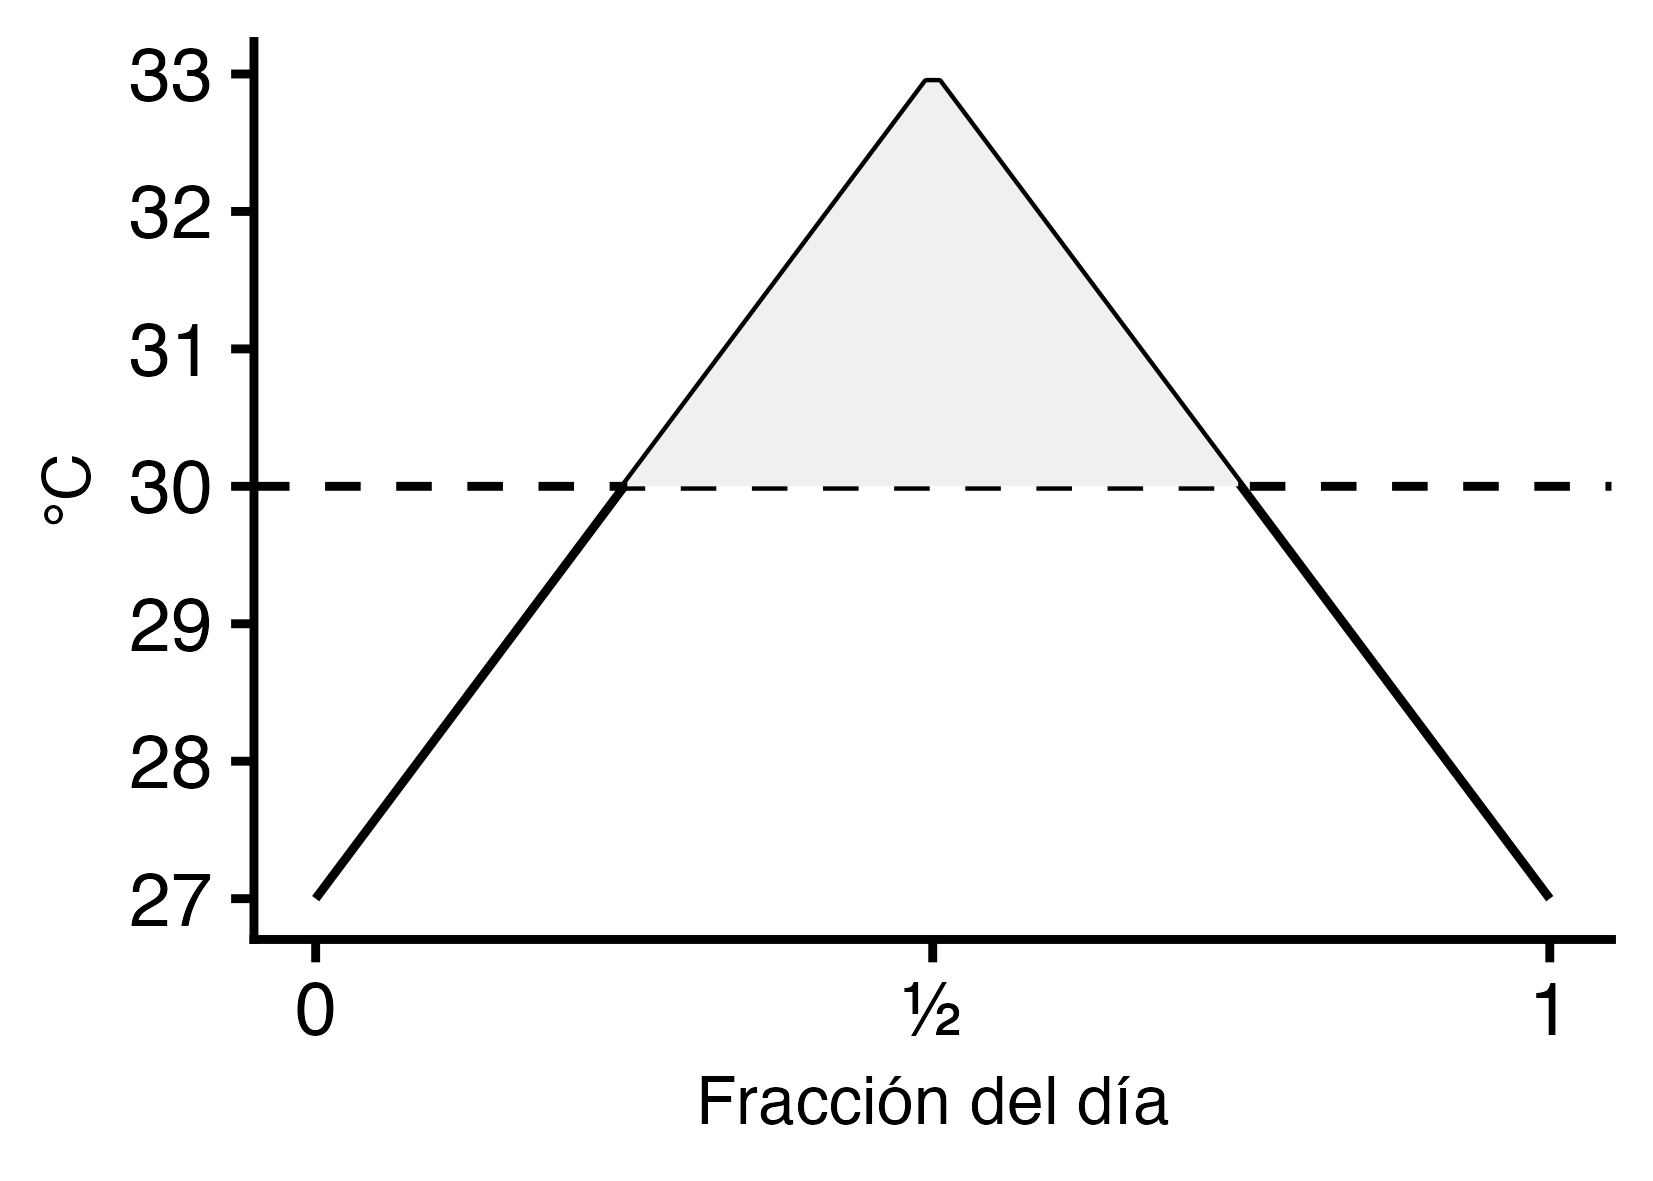
\includegraphics[width=\linewidth]{figures/exp_p5}
        \label{fig:exp_p5}
    \end{minipage}
\end{figure}
\end{frame}

\begin{frame}{Apéndice}{Variable de estrés térmico \hyperlink{frame:datos}{\beamerbutton{Volver}}}
\begin{figure}[H]
    \centering
    \begin{minipage}[t]{0.45\textwidth}
        \centering
        \caption{Sin exposición al frío}
        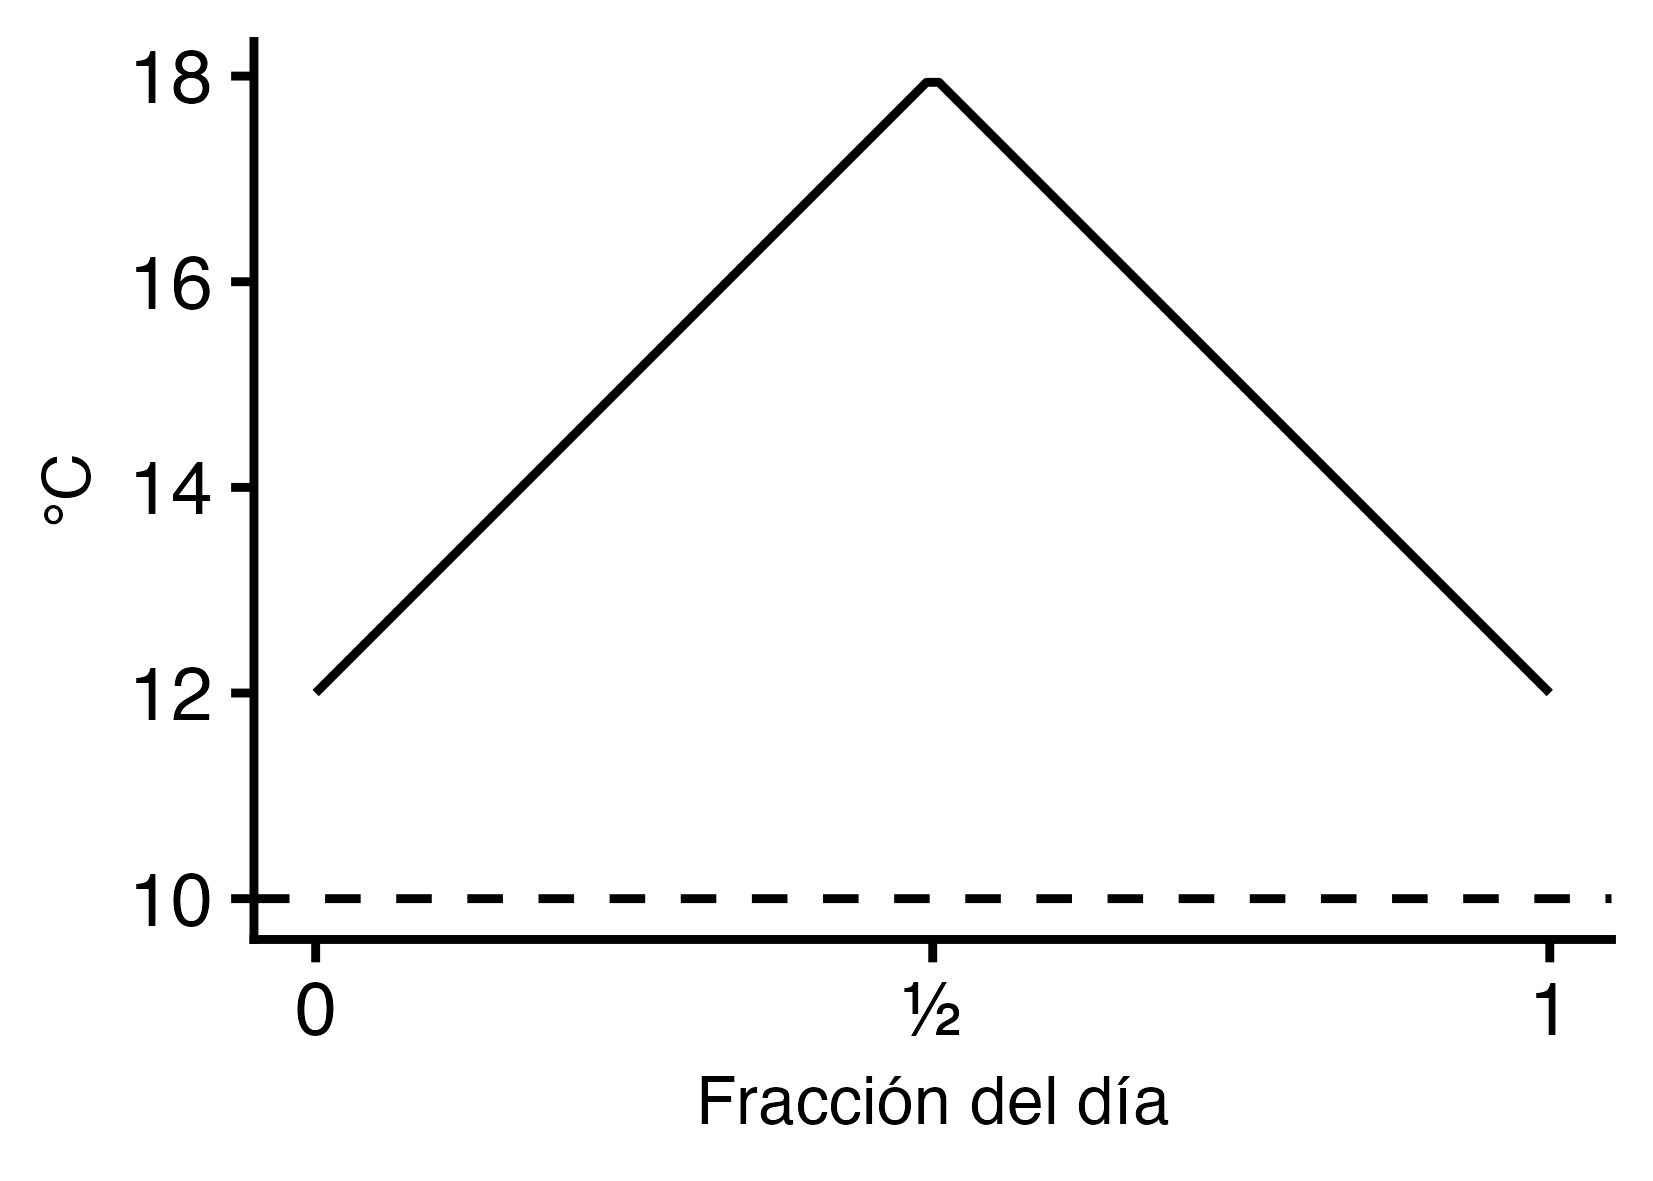
\includegraphics[width=\linewidth]{figures/exp_p3}
        \label{fig:exp_p3}
    \end{minipage}
    \hfill
    \begin{minipage}[t]{0.45\textwidth}
        \centering
        \caption{Exposición total al calor}
        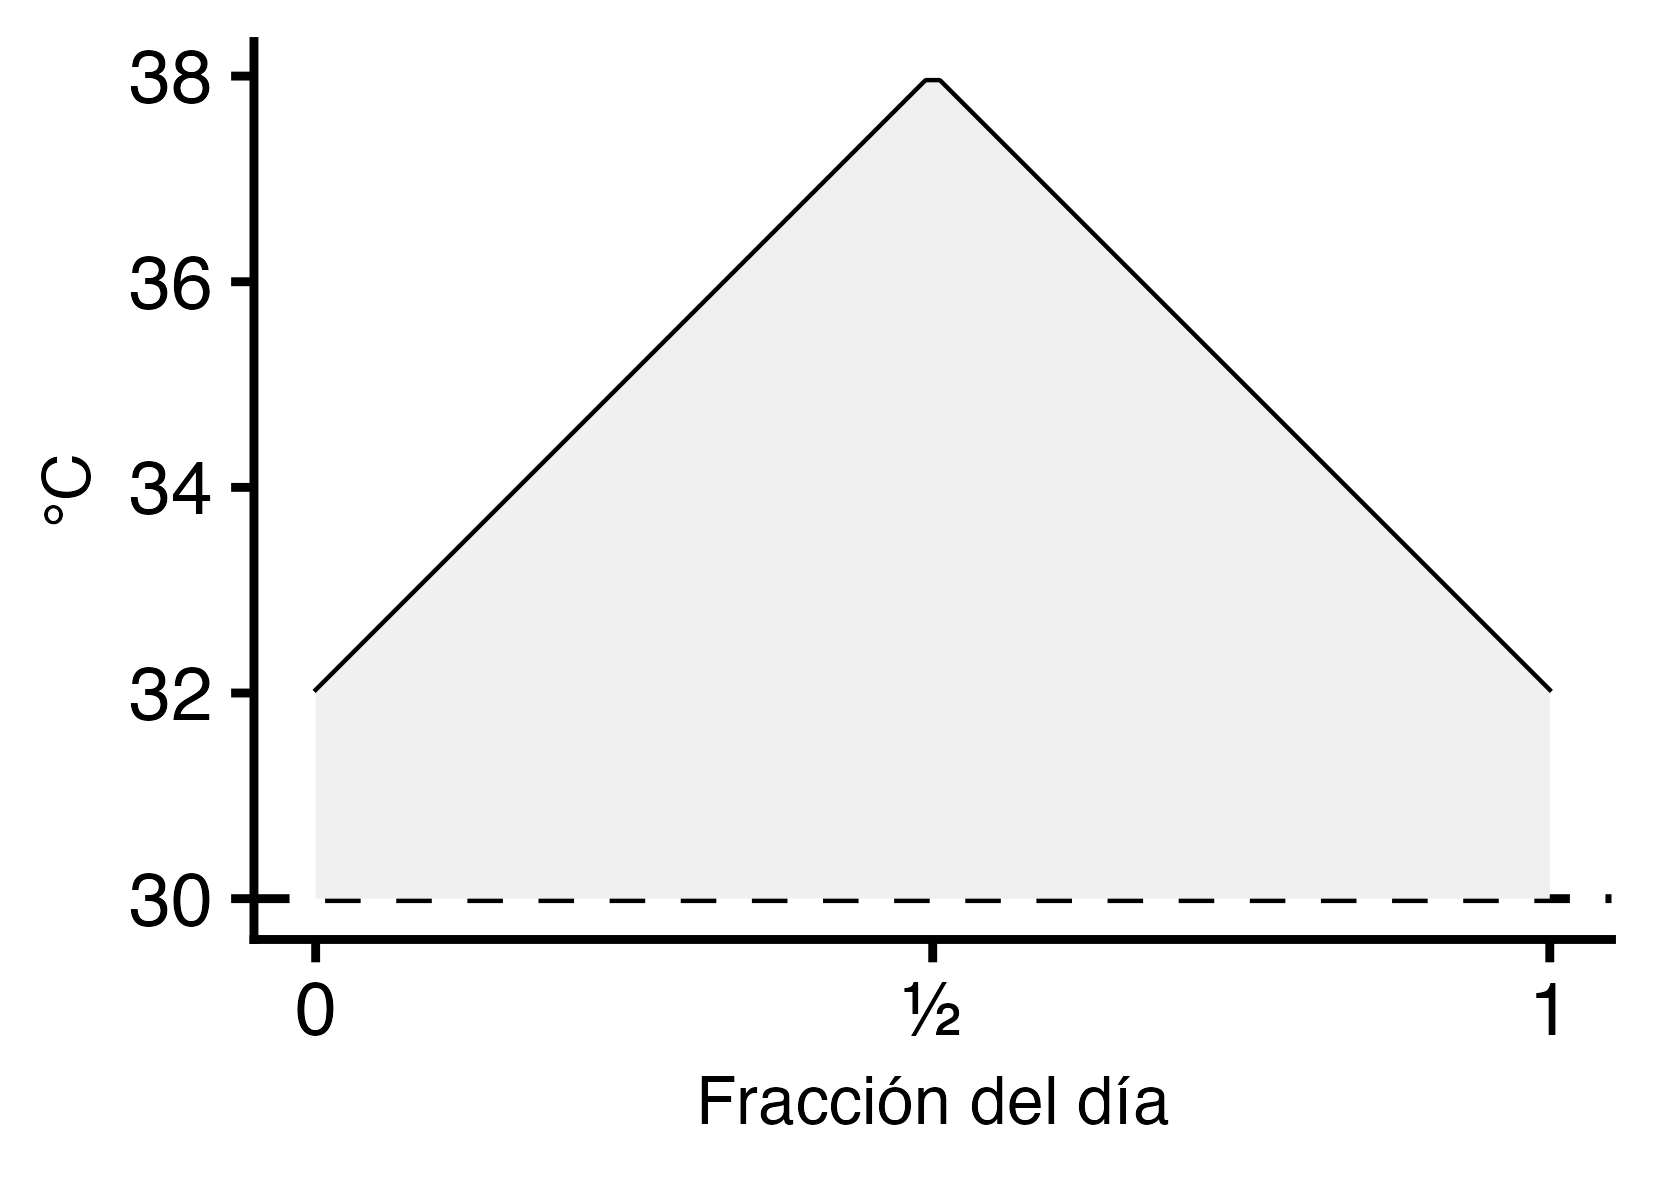
\includegraphics[width=\linewidth]{figures/exp_p6}
        \label{fig:exp_p6}
    \end{minipage}
\end{figure}
\end{frame}

\begin{frame}{Apéndice}{Variable de estrés térmico \hyperlink{frame:datos}{\beamerbutton{Volver}}}
\begin{figure}[H]
    \centering
    \begin{minipage}[t]{0.45\textwidth}
        \centering
        \caption{Exposición al óptimo en el tiempo}
        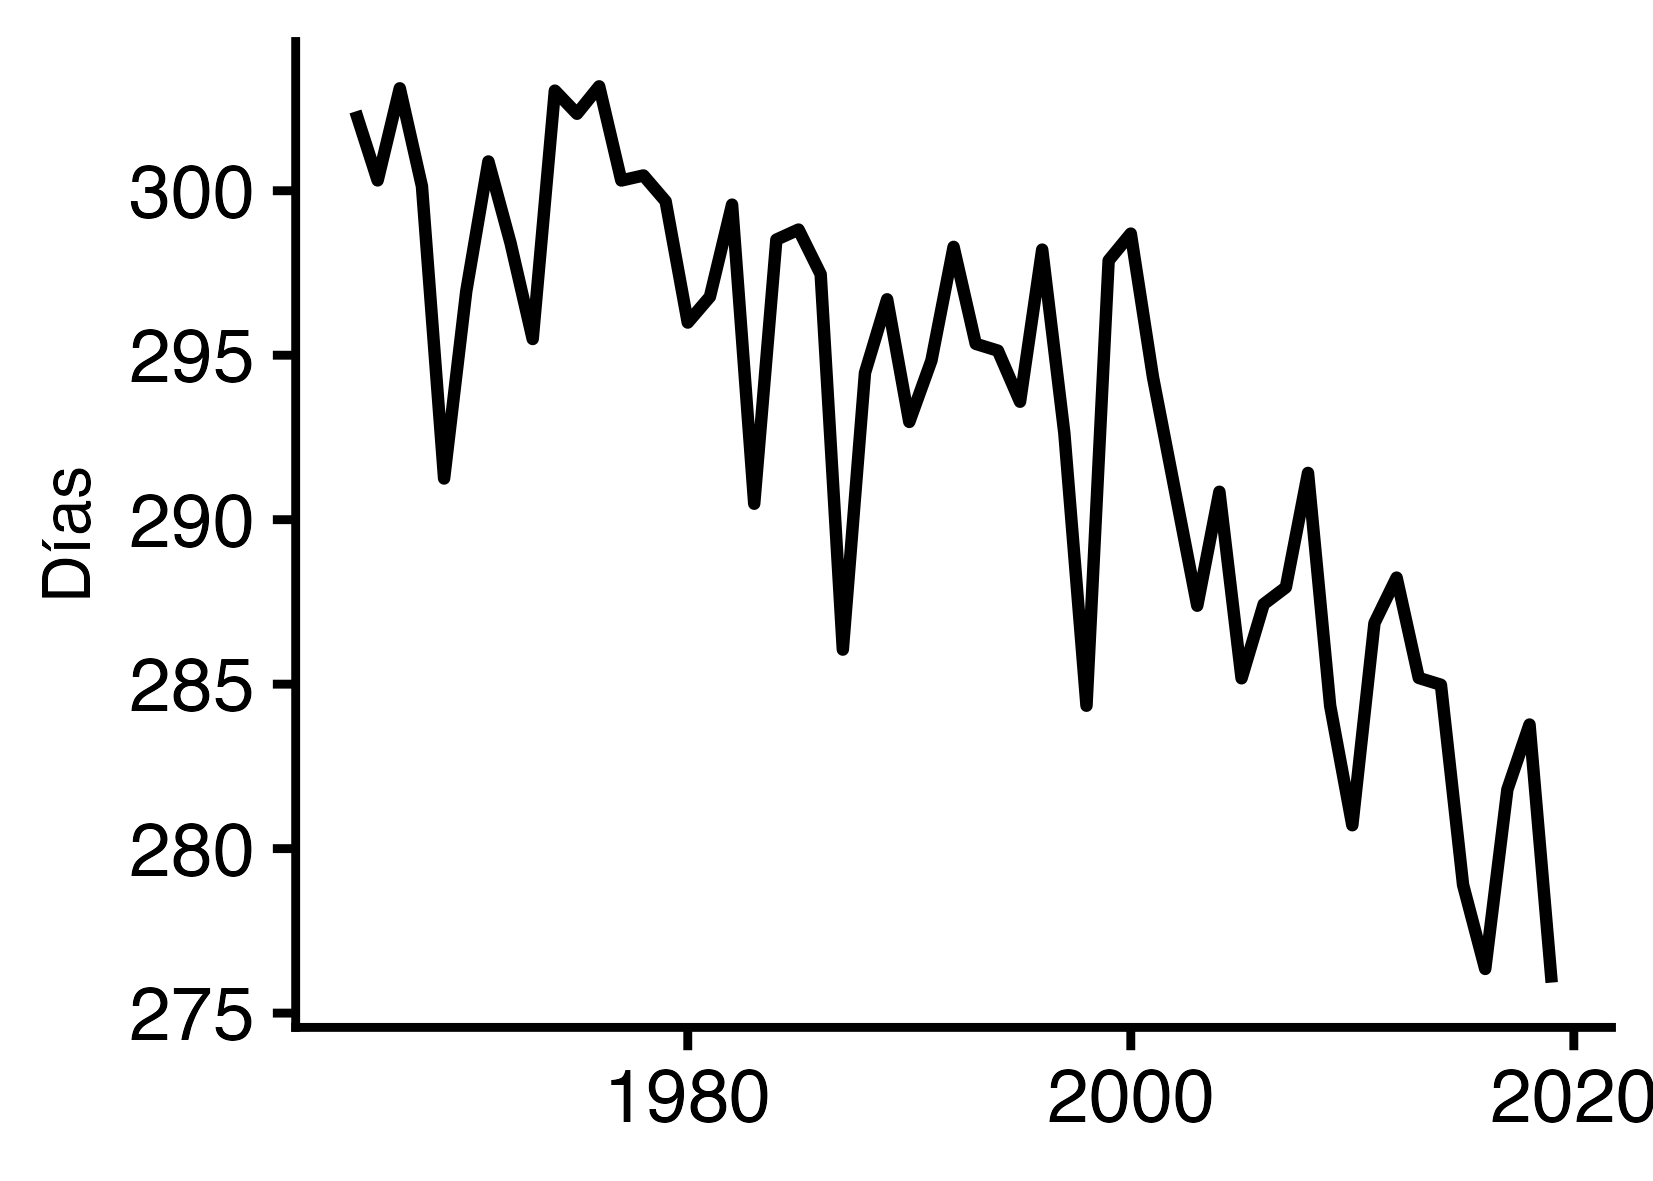
\includegraphics[width=\linewidth]{figures/optimo_y}
        \label{fig:optimo_y}
    \end{minipage}
    \hfill
    \begin{minipage}[t]{0.45\textwidth}
        \centering
        \caption{Exposición al frío en el tiempo}
        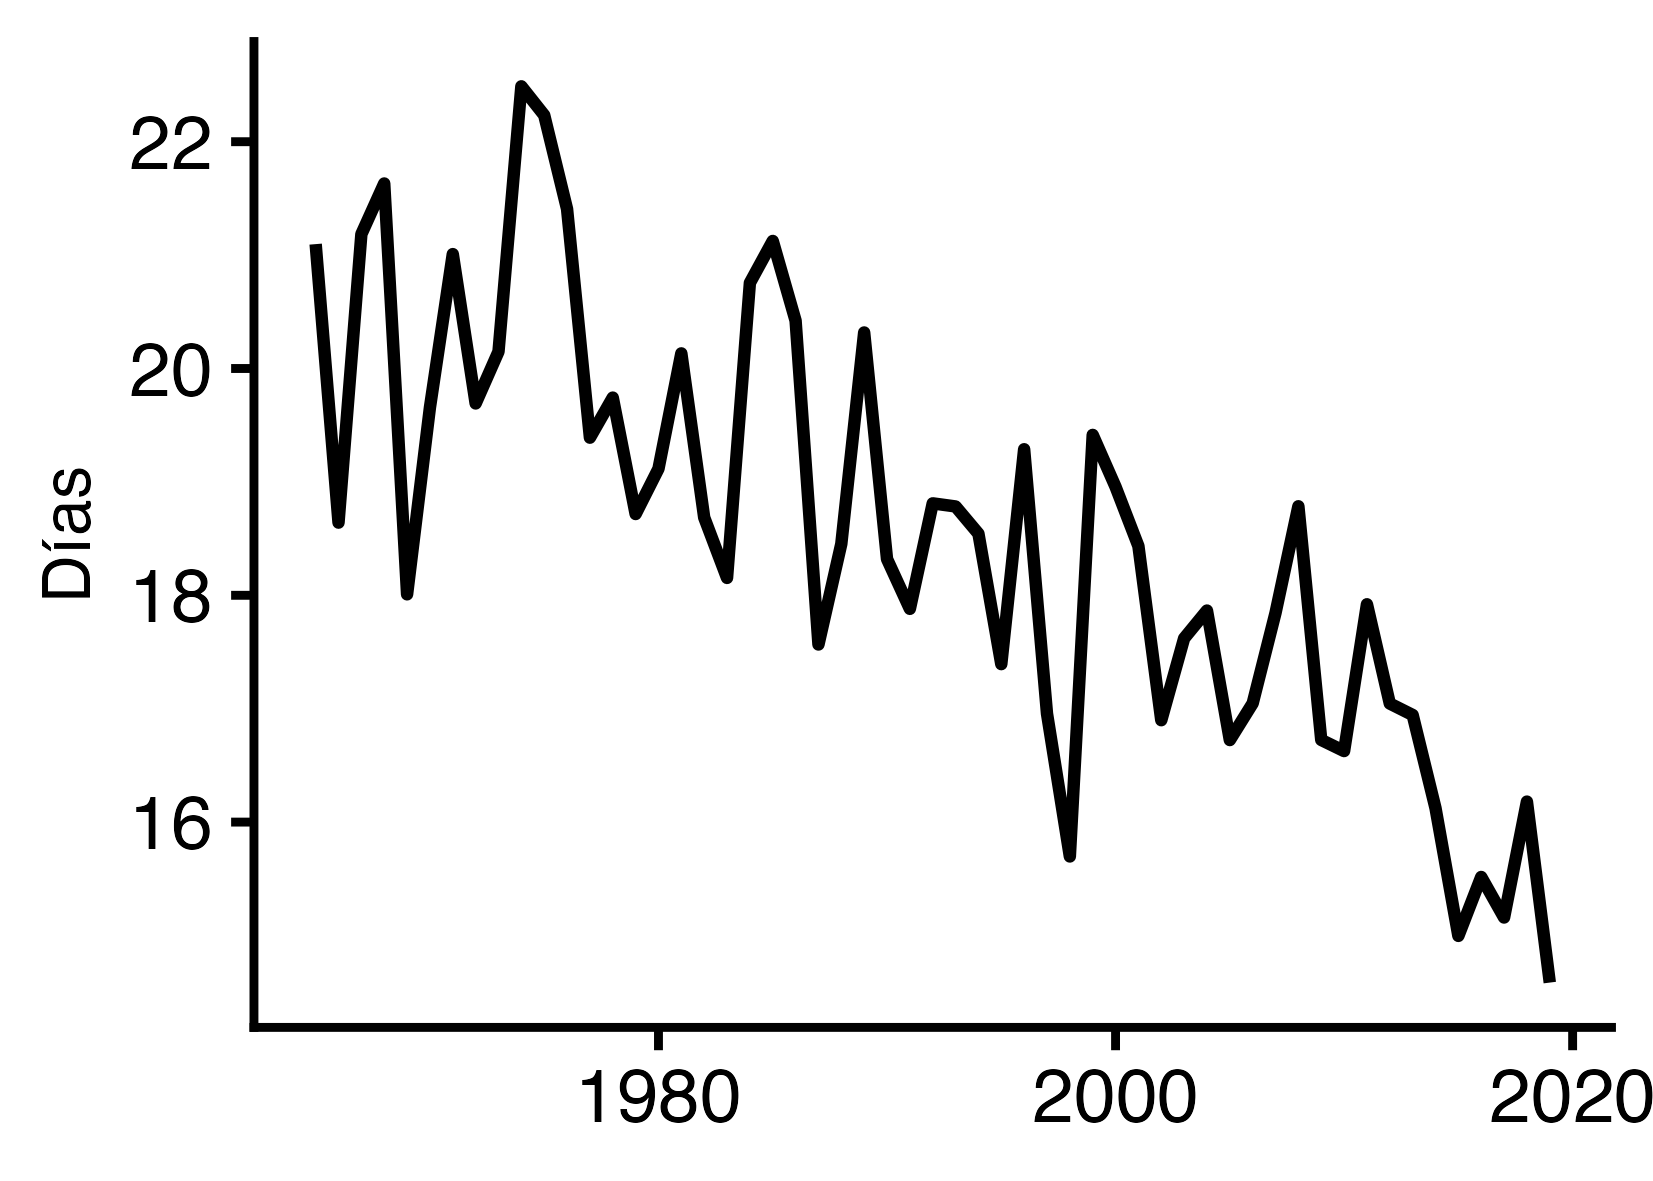
\includegraphics[width=\linewidth]{figures/frio_y}
        \label{fig:frio_y}
    \end{minipage}
\end{figure}
\end{frame}

\begin{frame}{Apéndice}{Variable de estrés térmico \hyperlink{frame:datos}{\beamerbutton{Volver}}} 
    
    \begin{figure}[H]
    \centering      
    \caption{Exposición al calor en el tiempo}
    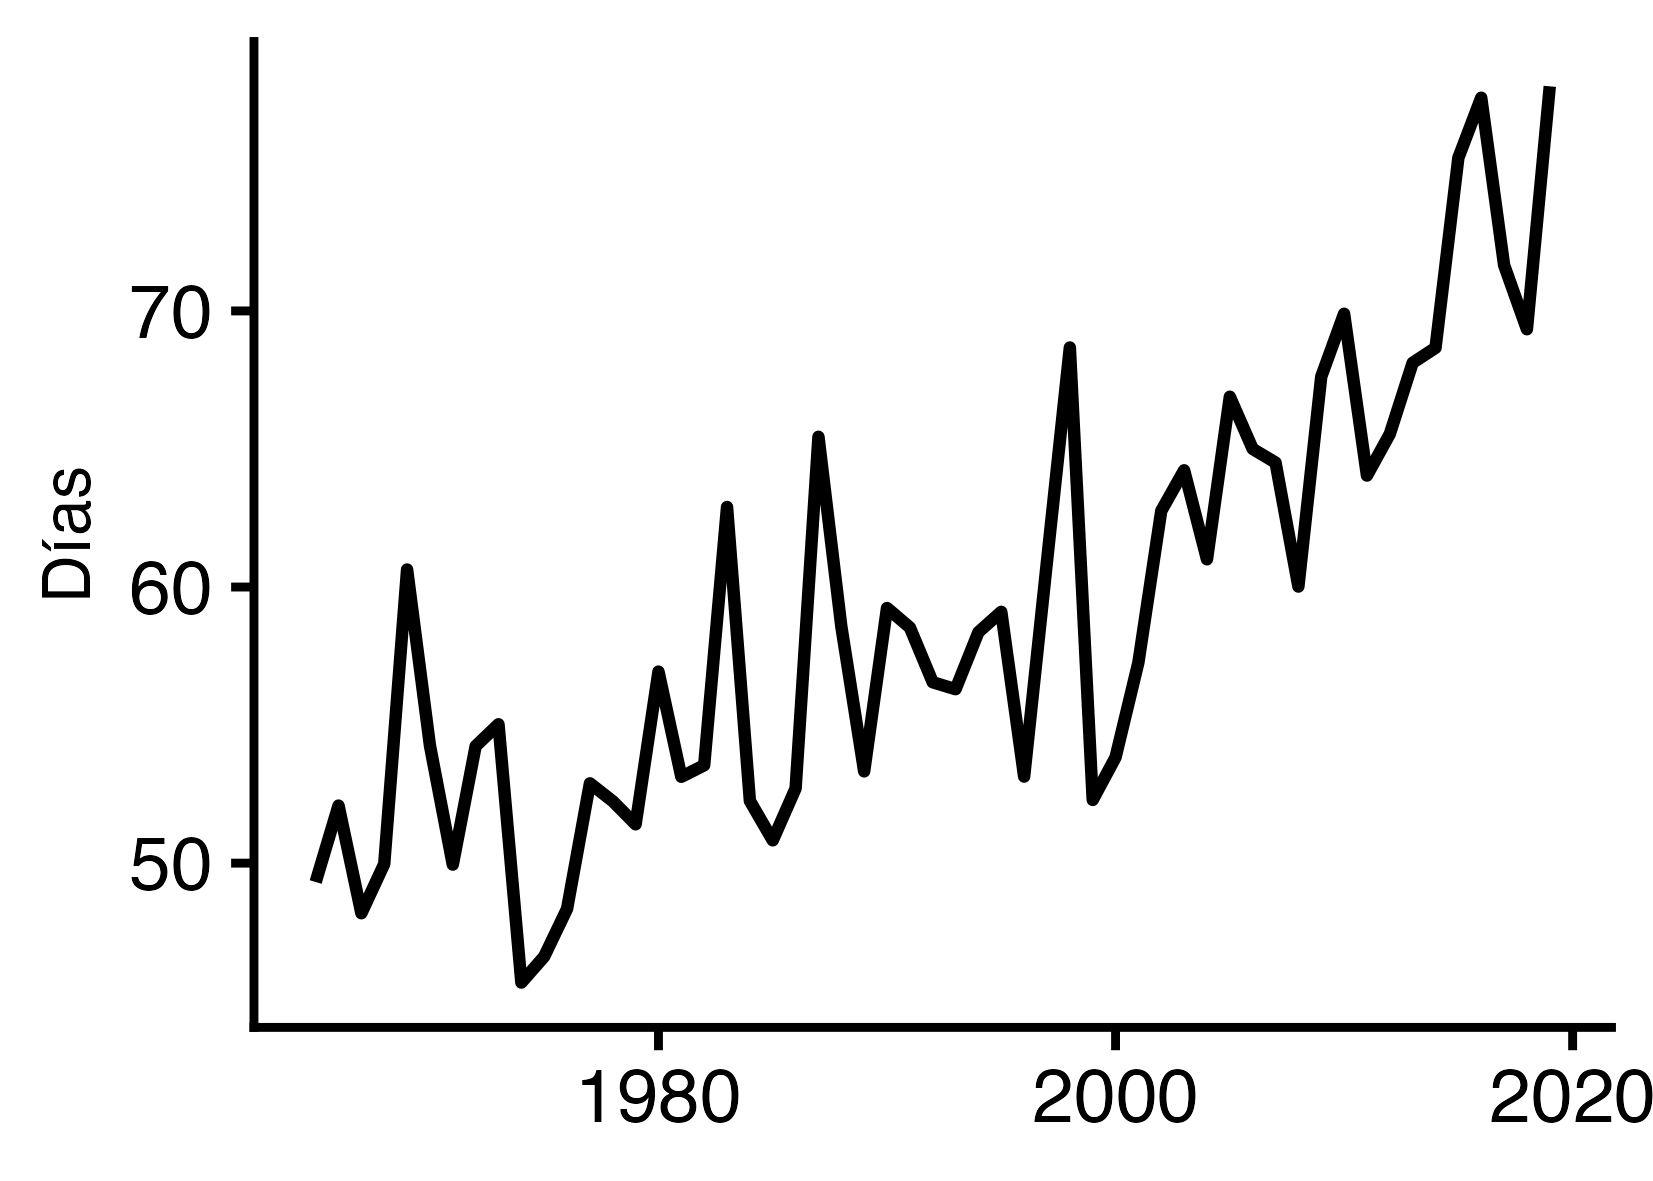
\includegraphics[scale=0.7]{figures/calor_y}
    \label{fig:calor_y}
    \end{figure}
\end{frame}

\begin{frame}{Apéndice}{Estimación de demanda mensual \hyperlink{frame:est_demand_y}{\beamerbutton{Volver}}}
\label{frame:est_demand_ym}
    \scriptsize
\begin{table}[H] \centering 
\caption{Estimaciones de la demanda mundial de café. Frecuencia mensual} 
\label{tab:est_demand_ym}
\begin{tabular}{@{\extracolsep{5pt}}lcc} 
\hline 
\hline 
Var. dep.: $P_{t}$ (Precio) & MCO & VI \\ 
\cline{2-3} 
\\[-1.8ex] 
$Q_{t}$ (Exportaciones de café)  & $-$111,5$^{***}$ & $-$213,9$^{***}$ \\ 
  & (7,8) & (57,0) \\ 
  & & \\ 
$X_{t}$ (PIB de importadores) & 305,3$^{***}$ & 593,6$^{***}$ \\ 
  & (23,9) & (160,8) \\ 
  & & \\ 
$Z_{t}$ (Precio del té) & 1,0$^{***}$& 1,1$^{***}$ \\ 
  & (0,0416) & (0,0920) \\ 
  & &\\ 
Constante & 194,2$^{***}$ & 424,7$^{***}$ \\ 
  & (31,3) & (131,5) \\ 
  & & \\ 
\hline \\[-1.8ex] 
Observaciones & 658 & 658 \\ 
R$^{2}$ aj. & 0,6607 & 0,5711 \\ 
F & 96,02$^{***}$ (df = 654) & \\ 
\hline 
\hline
\end{tabular}
\end{table}
\end{frame}



\begin{frame}{Apéndice}{Estimación de demanda. Primera etapa \hyperlink{frame:est_demand_y}{\beamerbutton{Volver}}}
\label{frame:est_demand_tests}
    \scriptsize
\begin{table}[H] \centering 
\caption{Estimación de demanda anual. Primera etapa} 
\label{tab:est_demand_y_1s}
\begin{tabular}{@{\extracolsep{5pt}}lc} 
\hline 
\hline 
    & $Q_{t}$ (Exportaciones de café) \\ 
\hline 
\\[-1.8ex] 
$T^{\text{máx}}_{t}$ (Temperatura máxima)& 0,66$^{**}$ \\ 
    & (0,2107)  \\ 
    & \\ 
$T^{\text{mín}}_{t}$ (Temperatura mínima)& $-$0,72$^{*}$ \\ 
    & (0,3210)  \\ 
    &  \\ 
$X_{t}$ (PIB de importadores) & 33,37$^{***}$ \\ 
    & (2,4480)\\ 
    & \\ 
$Z_{t}$ (Precio del té) & 0,02$^{.}$\\ 
    & (0,0088) \\ 
    & \\ 
Constante & $-$142,50$^{***}$ \\ 
    & (53,60) \\ 
    & \\ 
\hline \\[-1.8ex] 
Observaciones & 55\\ 
R$^{2}$ aj. & 0,9264  \\
F & 170.9 (p < 0.001)  \\
\hline 
\hline
\end{tabular}
\end{table}


\end{frame}
\begin{frame}{Apéndice}{Estimación de demanda. Pruebas estadísticas \hyperlink{frame:est_demand_y}{\beamerbutton{Volver}}}
    \input{tables/est_demand_y_tests}
    \input{tables/est_demand_ym_tests}

\end{frame}

\begin{frame}{Apéndice}{Estimación de demanda. Intervalo CLR \hyperlink{frame:est_demand_y}{\beamerbutton{Volver}}}
    \label{frame:est_demand_iv_weak}
    \setbeamertemplate{itemize items}[circle]
    \begin{wideitemize}
        \item Esta sección resuelve el sistema utilizando las cotas del intervalo de confianza CLR (\textit{Conditional Likelihood Ratio}), robusto a instrumentos débiles.
        \item El intervalo de confianza al 95\% mantiene coeficientes negativos. El objetivo es analizar el cambio en los resultados finales.

    $$ CLR = \left[ -42,07088 -7,05283 \right] $$

    \end{wideitemize}
    
    \end{frame}

\begin{frame}{Apéndice}{Intervalo CLR}
    \scriptsize
\begin{table}\centering

\caption{Estimación de costos marginales implícitos. Intervalo de confianza CLR}
\label{tab:est_cost_clr}

\begin{tabular}{lccc}
\hline 
\hline 
   \multicolumn{1}{c}{\textbf{Variable}} & \textbf{(1)} & \textbf{$CLR_{-42,07088}$} & \textbf{$CLR_{-7,05283}$} \\
   \midrule
   Tendencia      & -9,86$^{***}$ & -6,38$^{***}$ & -9,96$^{***}$ \\
                  & (0,8107)      & (0,8247) & (0,6238) \\
   \addlinespace
   Fertilizantes  & 0,51$^{***}$  & 0,37$^{***}$ & 0,52$^{***}$ \\
                  & (0,0174)      & (0,0425) & (0,0090) \\
   \addlinespace
   \textbf{Exposición al calor:} \\
   \quad (t)      & 0,42$^{***}$  & 0,40$^{***}$ & 0,38$^{**}$ \\
                  & (0,1043)      & (0,1088) & (0,1074) \\
   \quad (t-1)    & 0,26$^{*}$    & 0,12 & 0,27$^{***}$ \\
                  & (0,1055)      & (0,1156) & (0,1003) \\
   \midrule
   Efectos fijos país & Sí & Sí & Sí \\
   Observaciones & 1.282 & 1.282 & 1.282 \\
   Adj. R$^2$ & 0,2651 & 0,3074 & 0,1519 \\
   Within R$^2$ & 0,0841 & 0,1392 & 0,1470 \\
\hline 
\hline 
\end{tabular}
\end{table}

\end{frame}
\begin{frame}{Apéndice}{Intervalo CLR}
    \scriptsize
\begin{table}[H]
\centering
\caption{Impacto del estrés térmico. Promedio anualizado 1990-2019}
\label{tab:results1_clr}
\begin{tabular}{lcc}
\hline
\textbf{Escenario} &
\textbf{\begin{tabular}[c]{@{}c@{}}Precio\\ (¢/lb)\end{tabular}} &
\textbf{\begin{tabular}[c]{@{}c@{}}Cantidad\\ (mill. 60 kg.)\end{tabular}} \\ \hline
Sin estrés térmico &
(130,0 -133,4) &
(38,8 - 230,9)  \\ 
Con estrés térmico &
(135,6 - 140,3) &
(38,7 -229,9) \\
\hline
Cambio & $\uparrow$(4,3\% - 5,2\%) & $\downarrow$(0,3\% 0,4\%)\\
\hline
\end{tabular}%
\end{table}
    \scriptsize
\begin{table}[H]
\centering
\caption{Impacto del estrés térmico. Promedio anualizado 1990-2019 (mill. USD)}
\label{tab:results2_clr}
\begin{tabular}{lcccc}
\hline
\textbf{Escenario} &
\textbf{\begin{tabular}[c]{@{}c@{}}Excedente\\ líderes \end{tabular}} &
\textbf{\begin{tabular}[c]{@{}c@{}}Excedente\\ seguidores\end{tabular}} &
\textbf{\begin{tabular}[c]{@{}c@{}}Excedente\\ importadores\end{tabular}} &
\textbf{\begin{tabular}[c]{@{}c@{}}Excedente\\ total\end{tabular}} \\ \hline
Sin estrés térmico &
(72,9 - 1.657)  &
(1.115 - 1.956)  &
(42.522 - 252.695) &
(43.710 - 256.308)  \\ 
Con estrés térmico &
(72,7 - 1.661)&
(1.101 -1.900)  &
(42.215 - 250.429)  &
(43.389 - 253.990)  \\
\hline
Cambio & $\downarrow$(0,3\% - 0,2\%) & $\downarrow$(1,3\% - 2,9\%) & $\downarrow$(0,7\% - 0,9\%) & $\downarrow$(0,7\% - 0,9\%) \\
\hline
\end{tabular}
\end{table}

\end{frame}

\begin{frame}{Apéndice}{Ajuste del modelo \hyperlink{frame:est_costs_y}{\beamerbutton{Volver}}}
    \label{frame:ajuste_modelo}
\begin{figure}[H]
    \centering
    \begin{minipage}[t]{0.45\textwidth}
        \centering
        \caption{Ajuste en precios}
        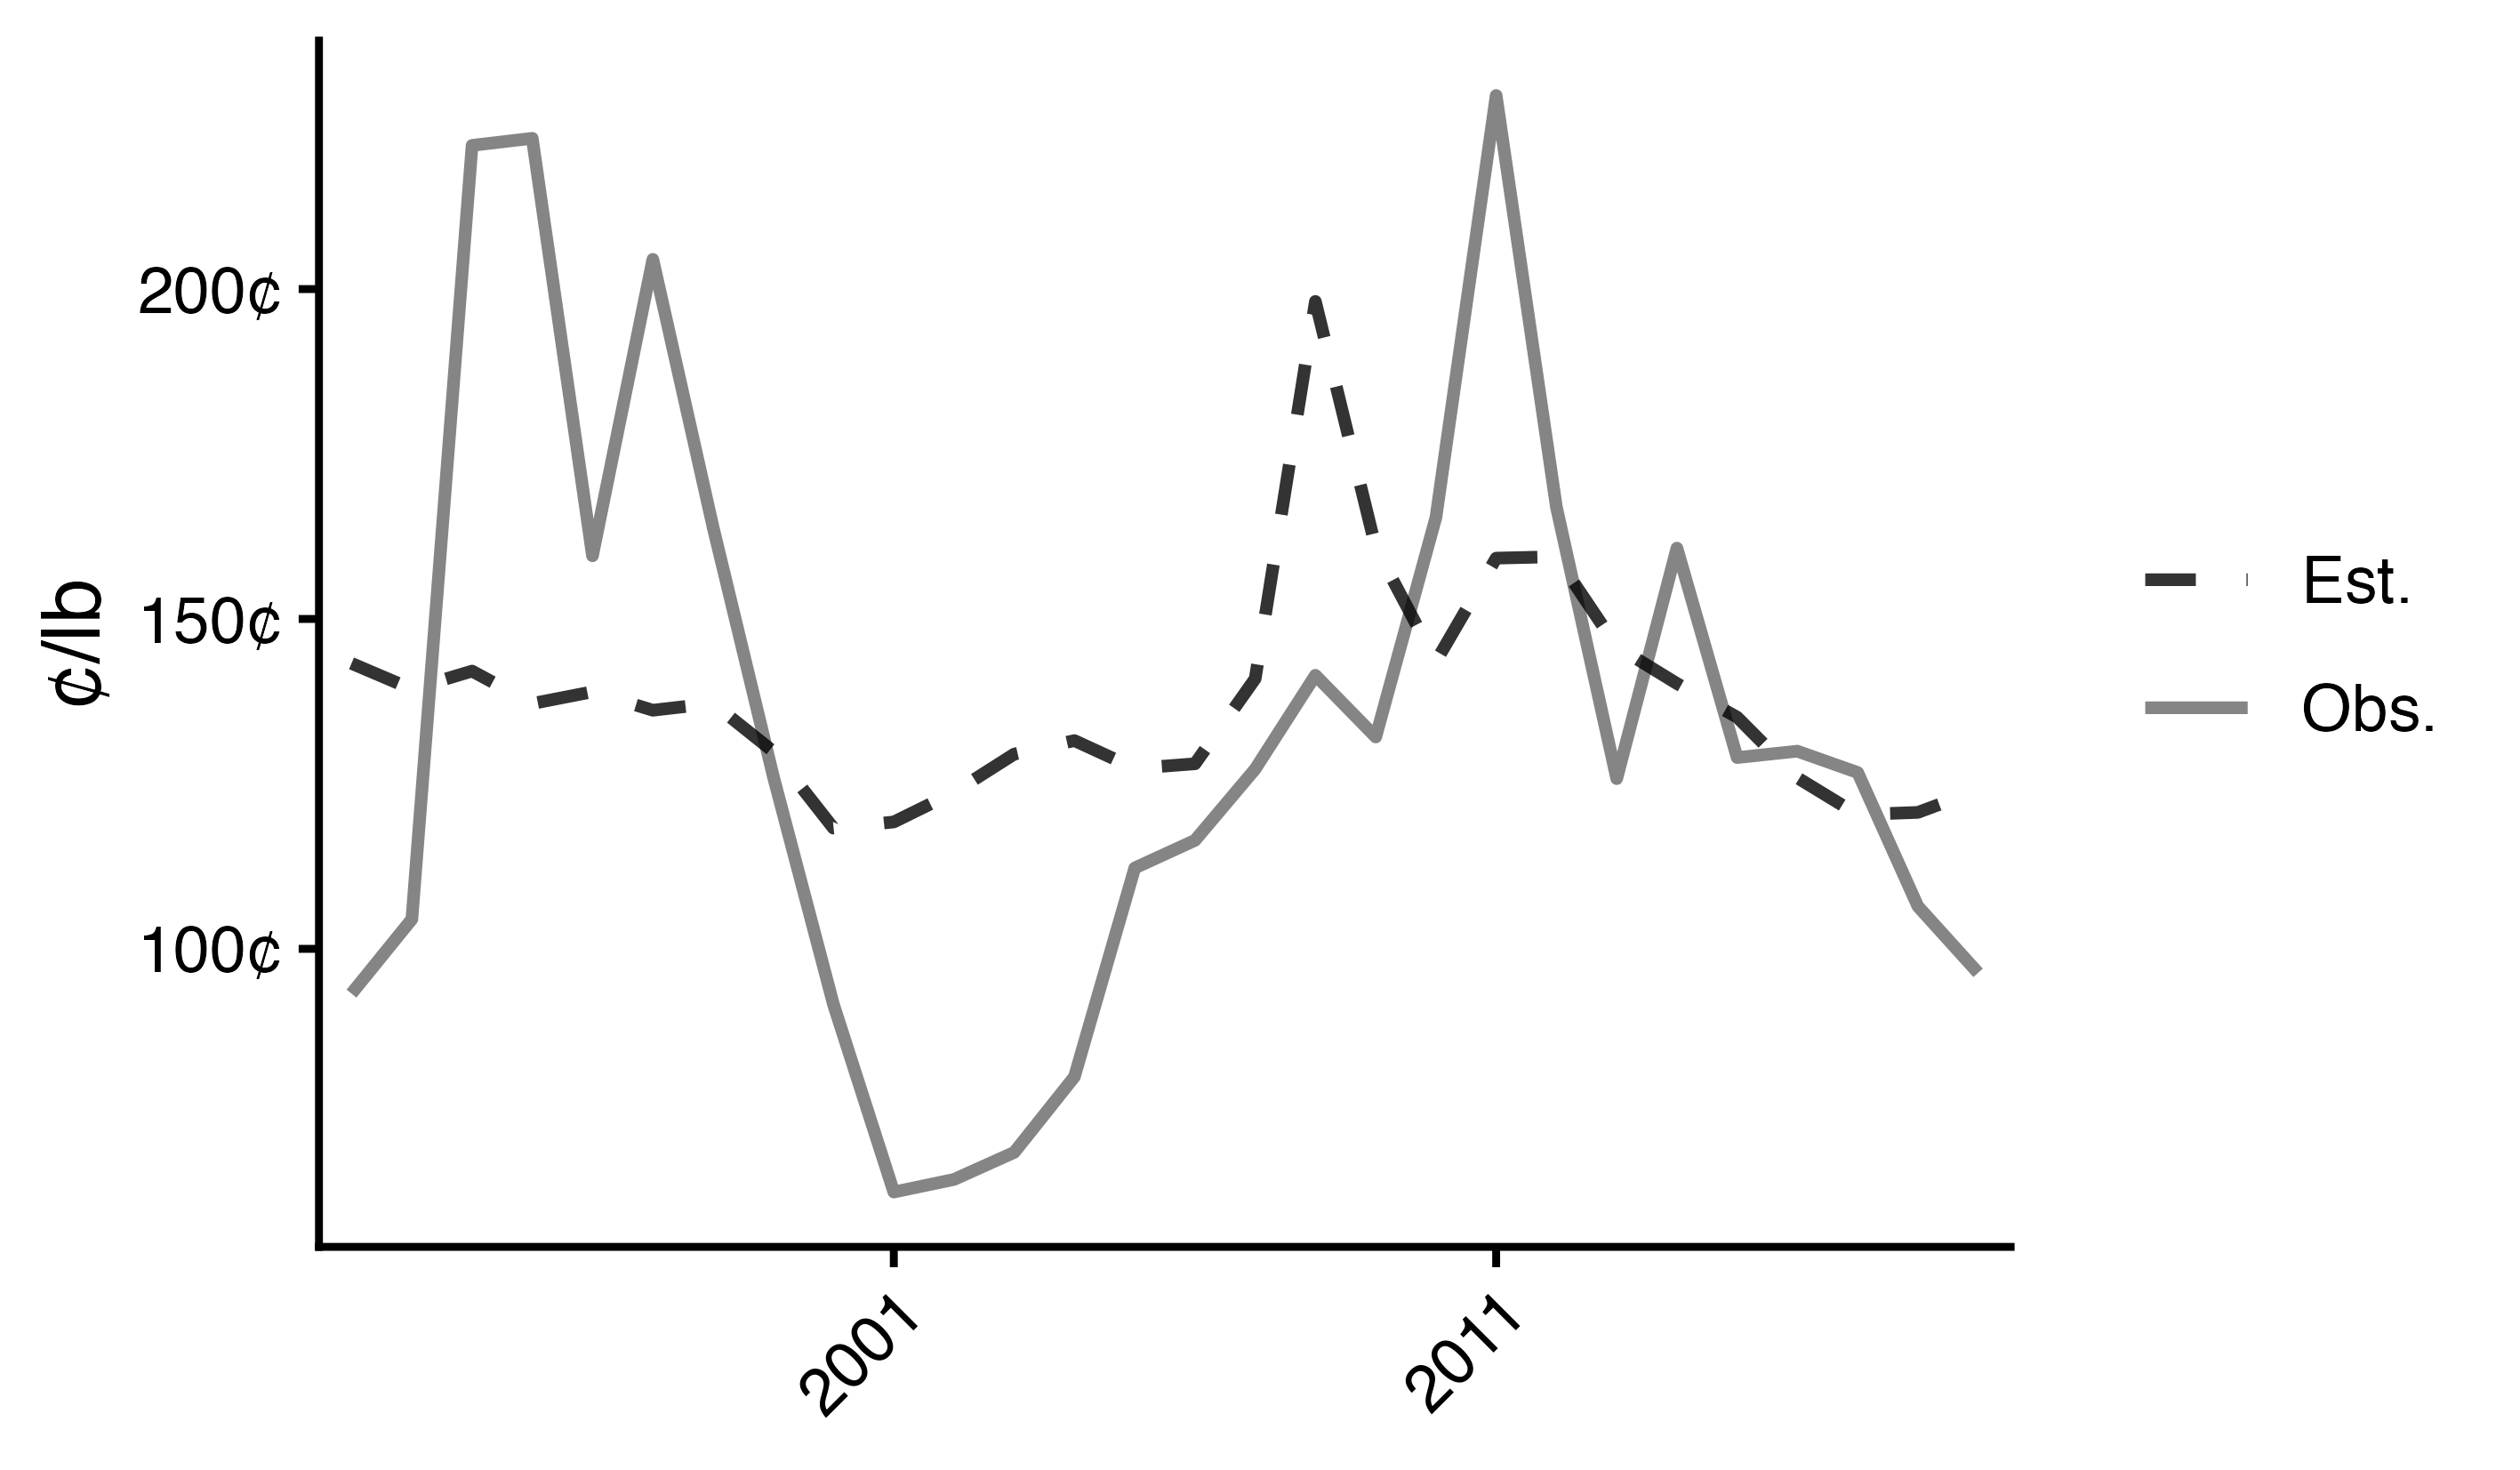
\includegraphics[width=\linewidth]{figures/fit_precio}
        \label{fig:fit_precio}
    \end{minipage}
    \hfill
    \begin{minipage}[t]{0.45\textwidth}
        \centering
        \caption{Ajuste en cantidades}
        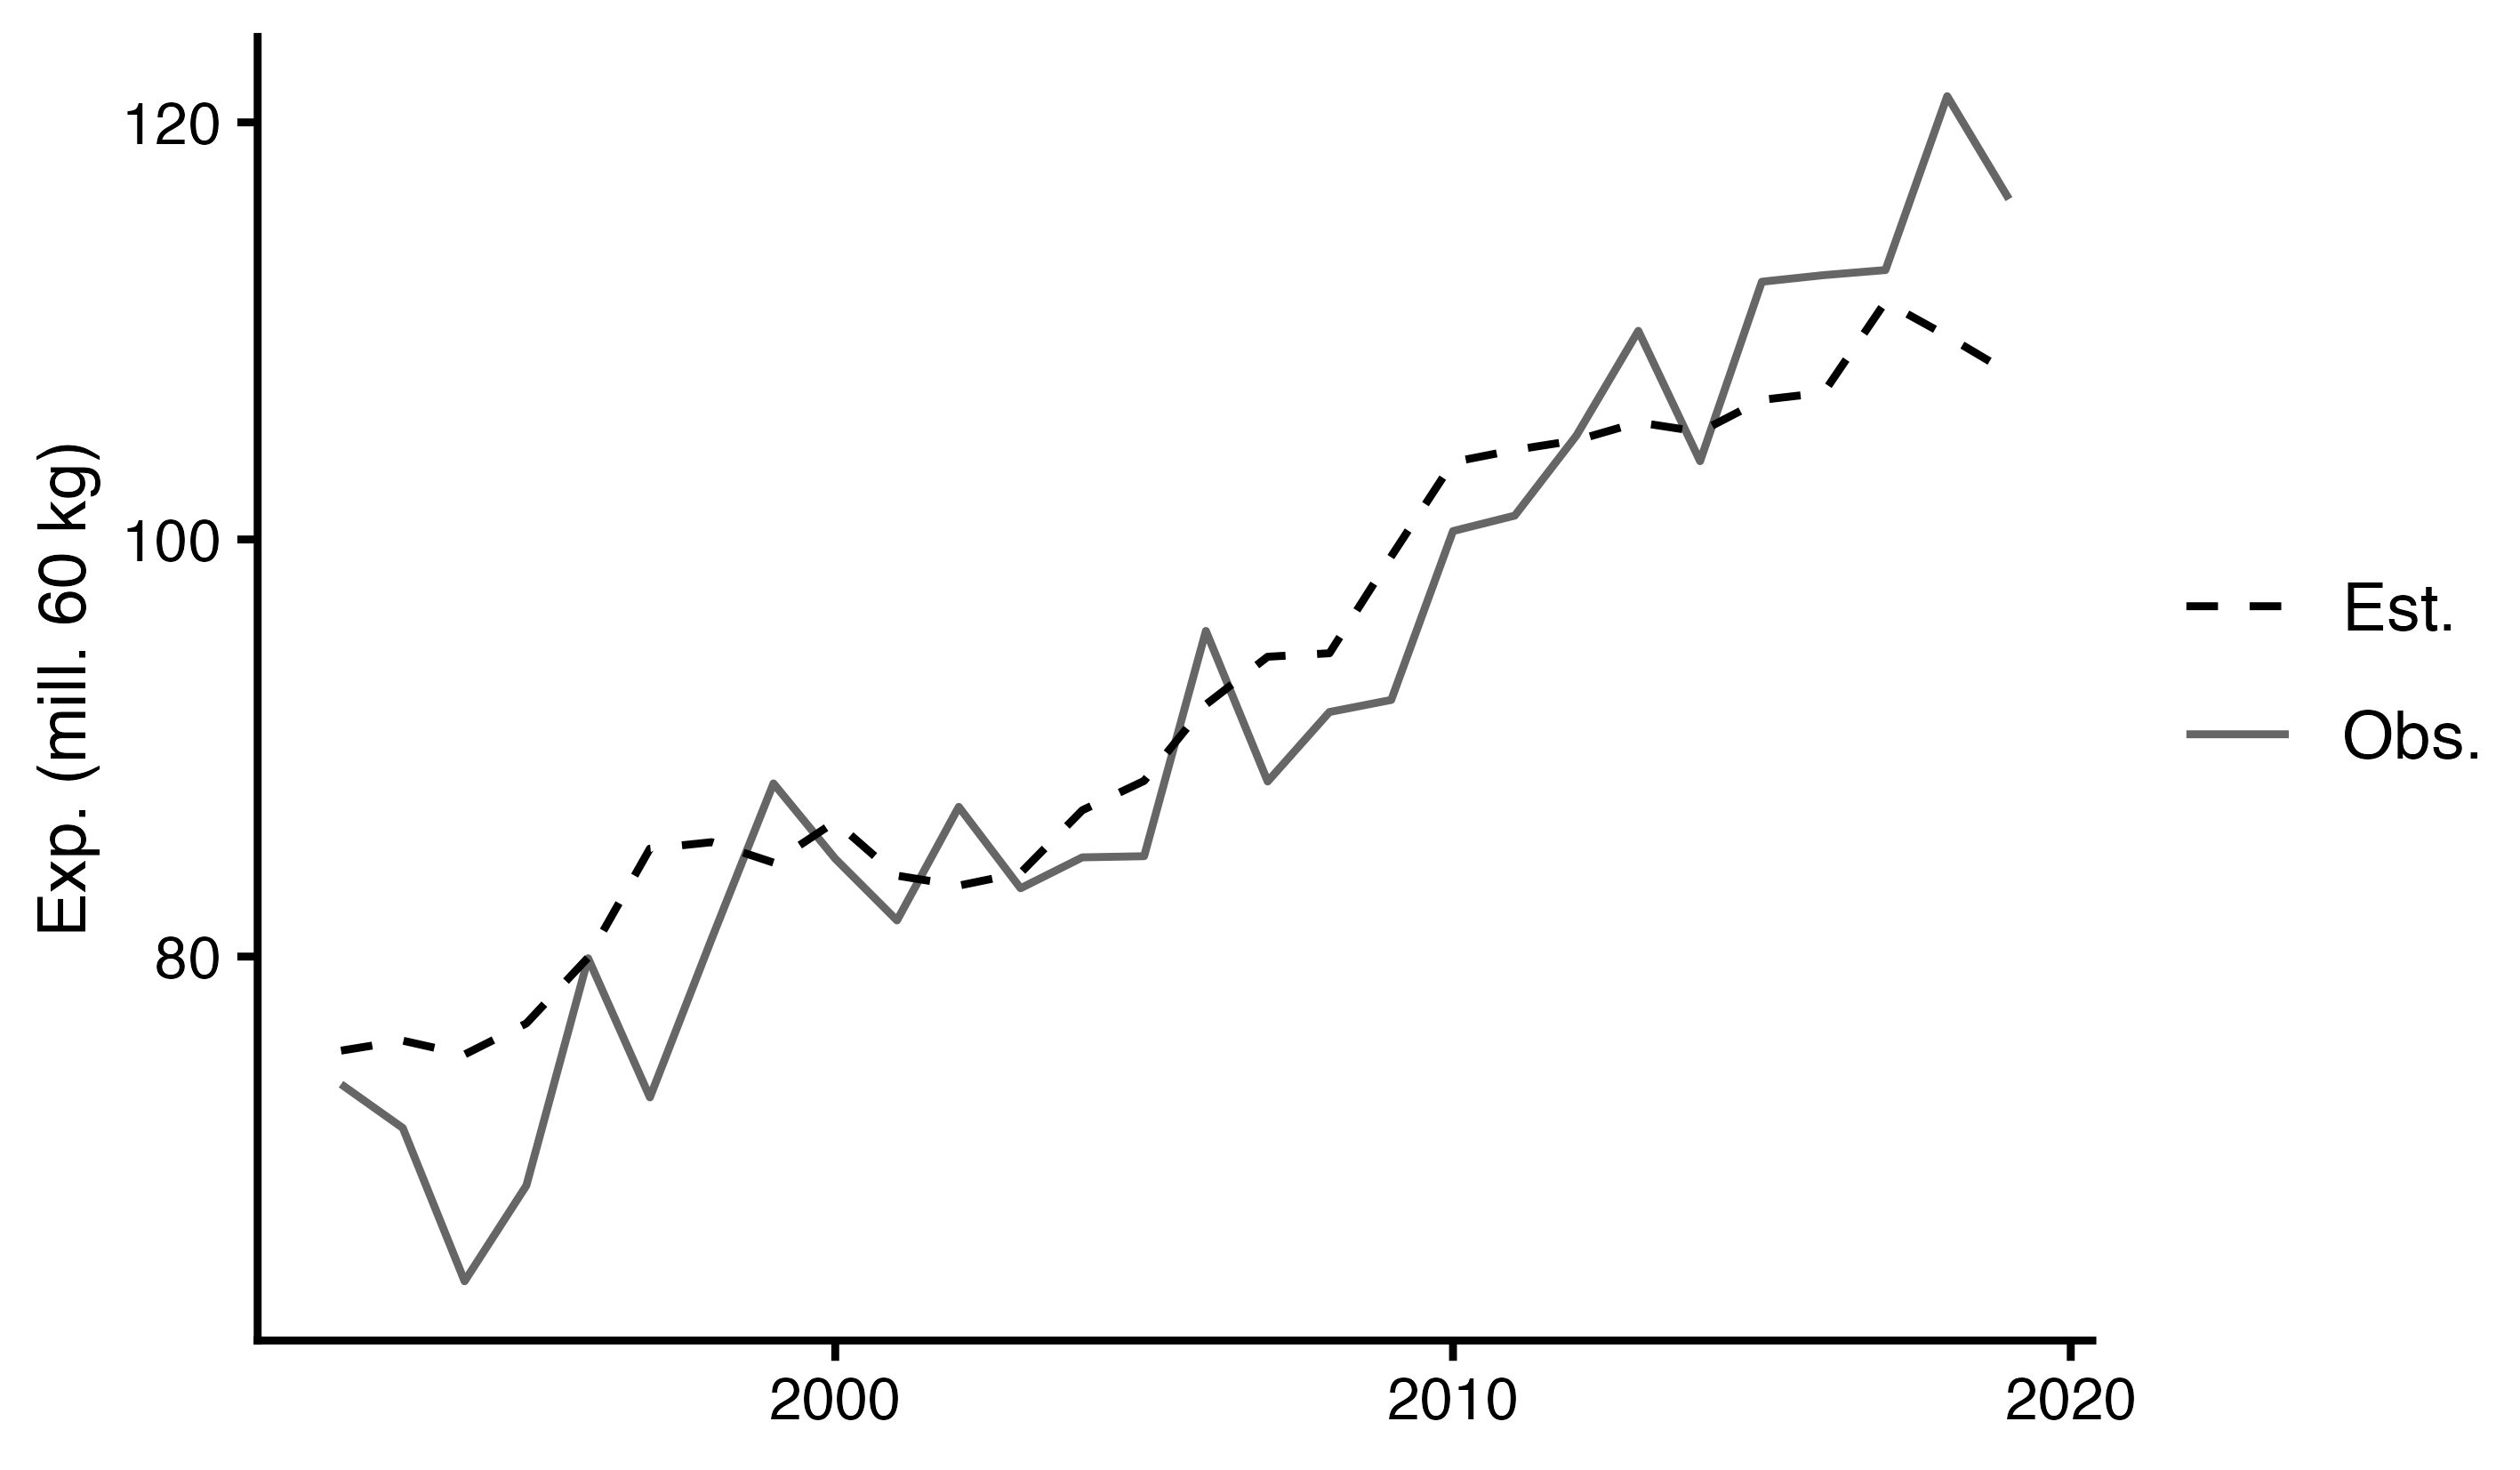
\includegraphics[width=\linewidth]{figures/fit_qe}
        \label{fig:fit_qe}
    \end{minipage}
\end{figure}
\end{frame}

\begin{frame}{Apéndice}{Estiamción de costos marginales \hyperlink{frame:est_costs_y}{\beamerbutton{Volver}}}
    \vspace{0.2cm}
\label{frame:est_costs_y_hist}
    \begin{figure}
        \caption{Histograma de costos marginales (1990-2019)}
        \centering
        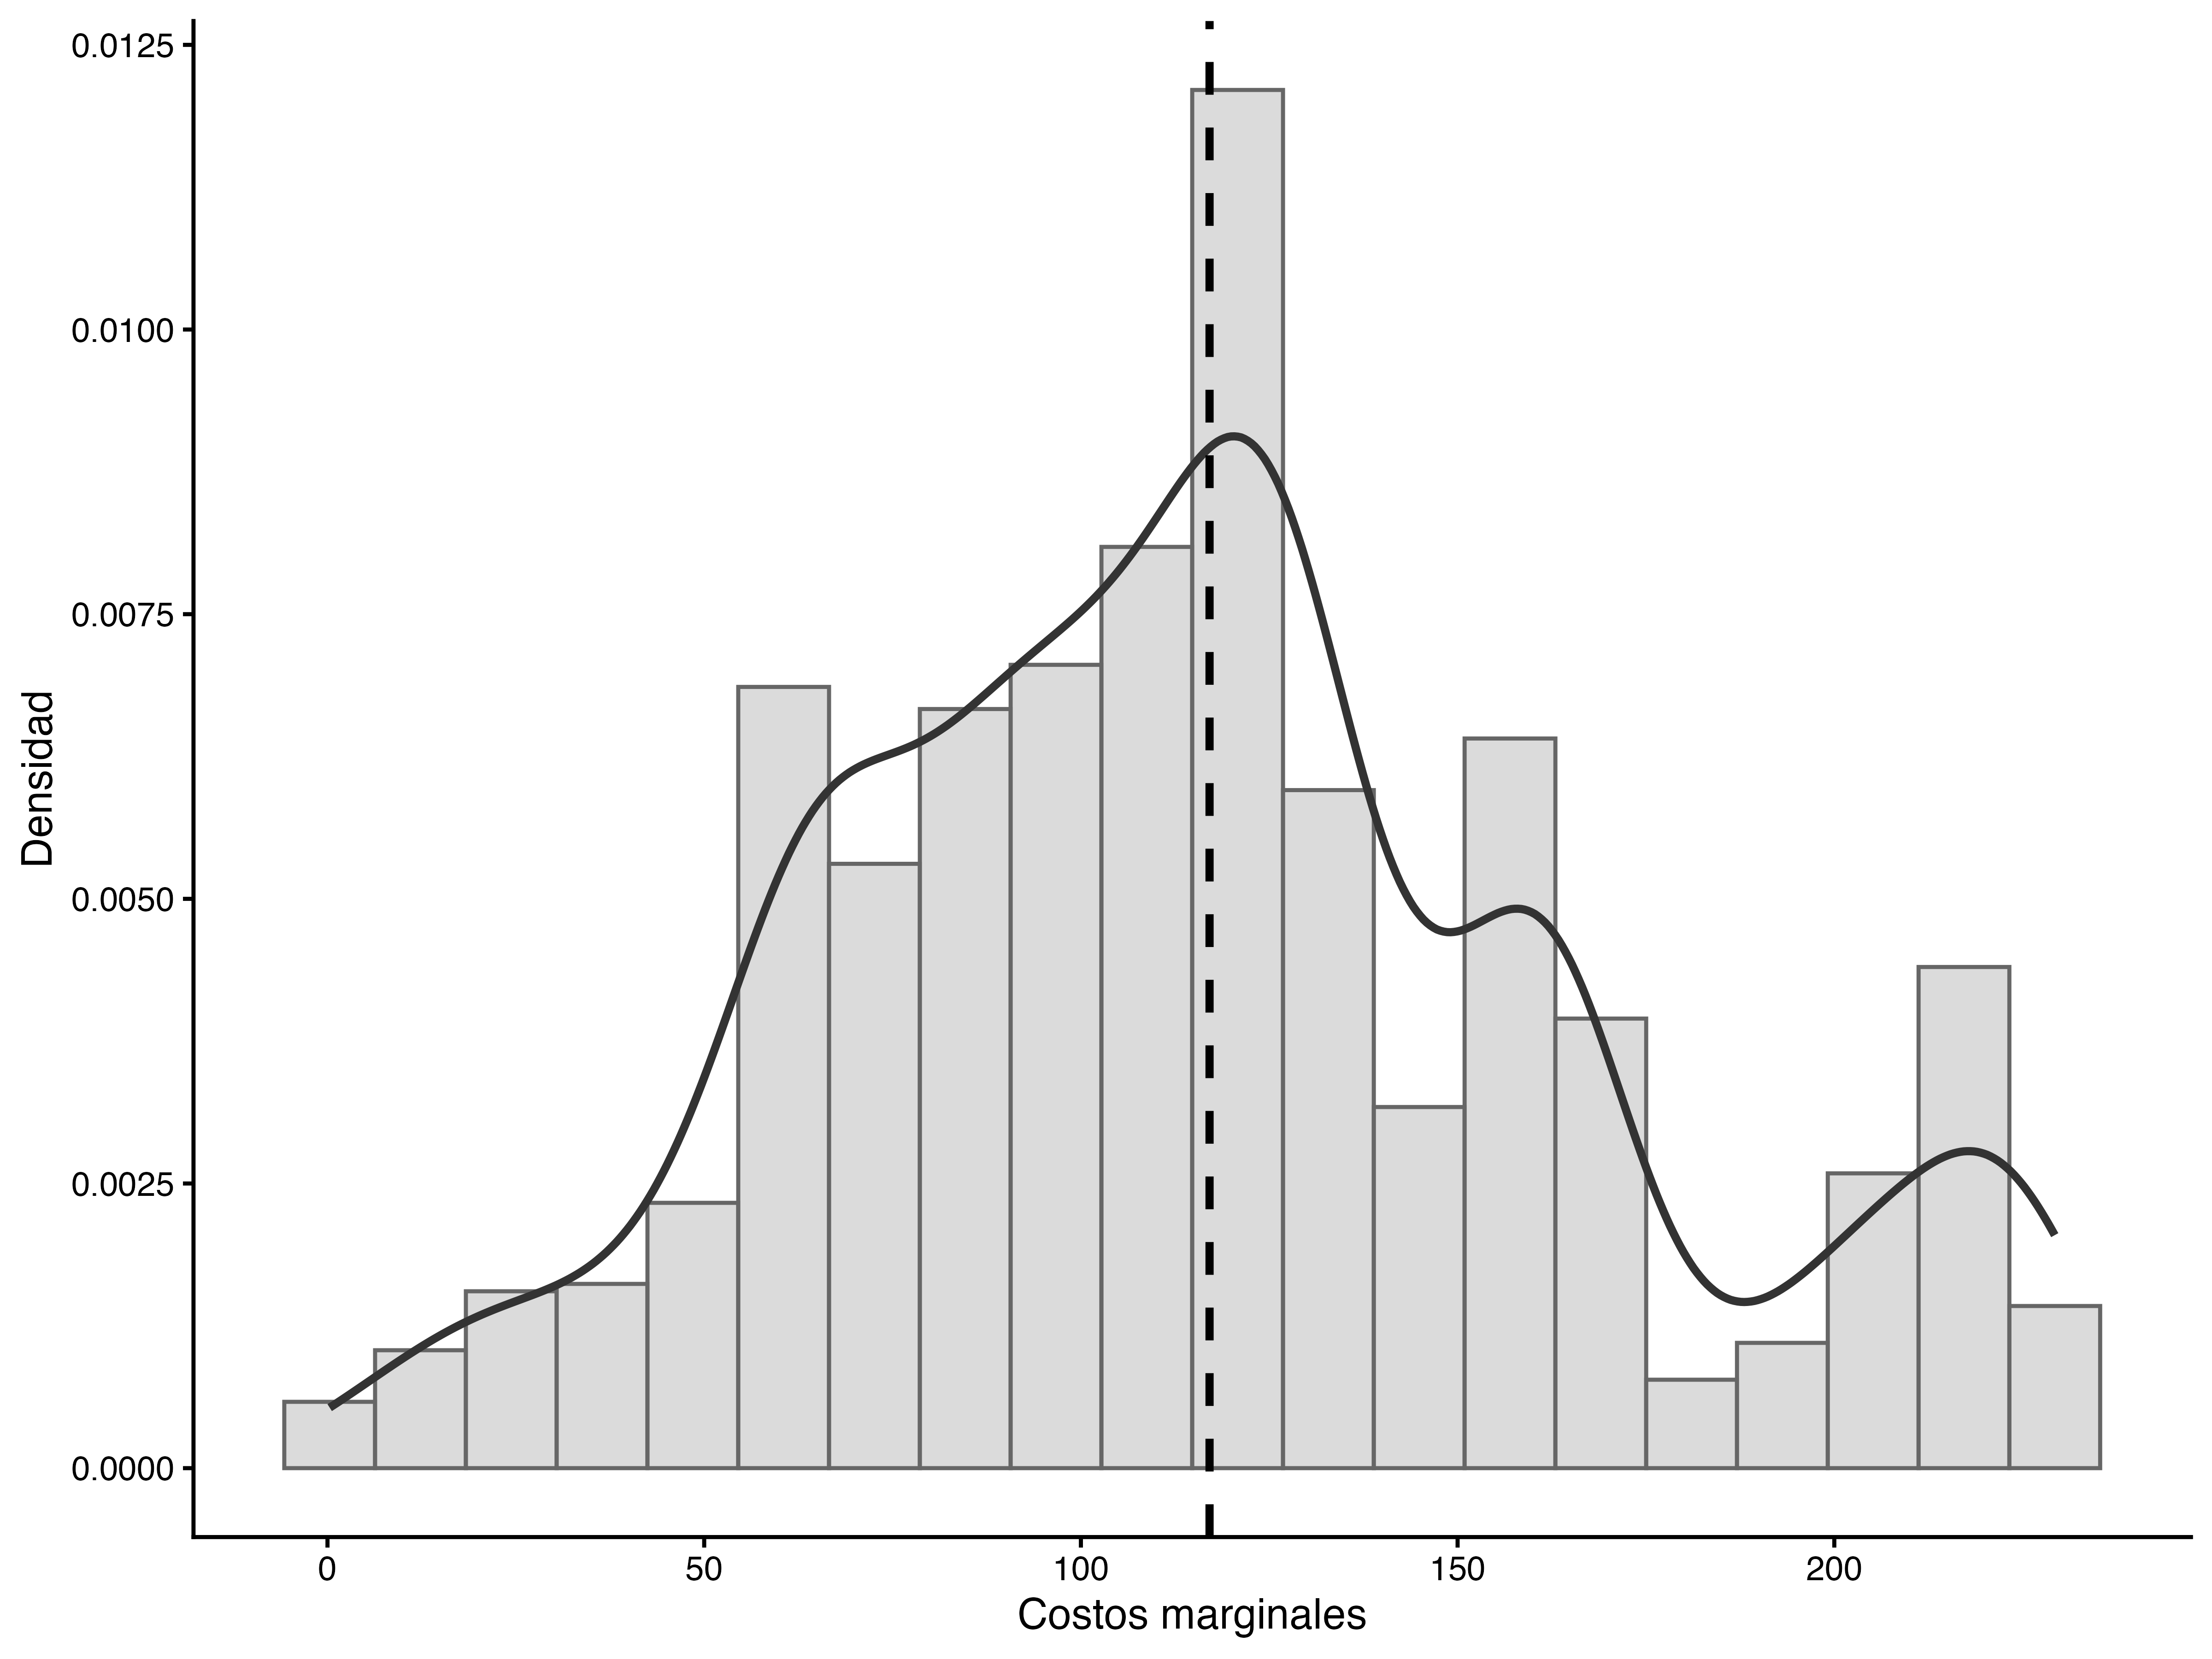
\includegraphics[scale=0.4]{figures/costs_hist}
    \end{figure}
\end{frame}

\begin{frame}{Apéndice}{Cambio en calor y costos. Resultados por país \hyperlink{frame:hallazgo2}{\beamerbutton{Volver}}}
    \label{frame:diff_heat_diff_costs}
    \begin{figure}[H]
        \caption{Cambio en calor y costos (1990-2019 vs. 1970-1989)}
    \centering
    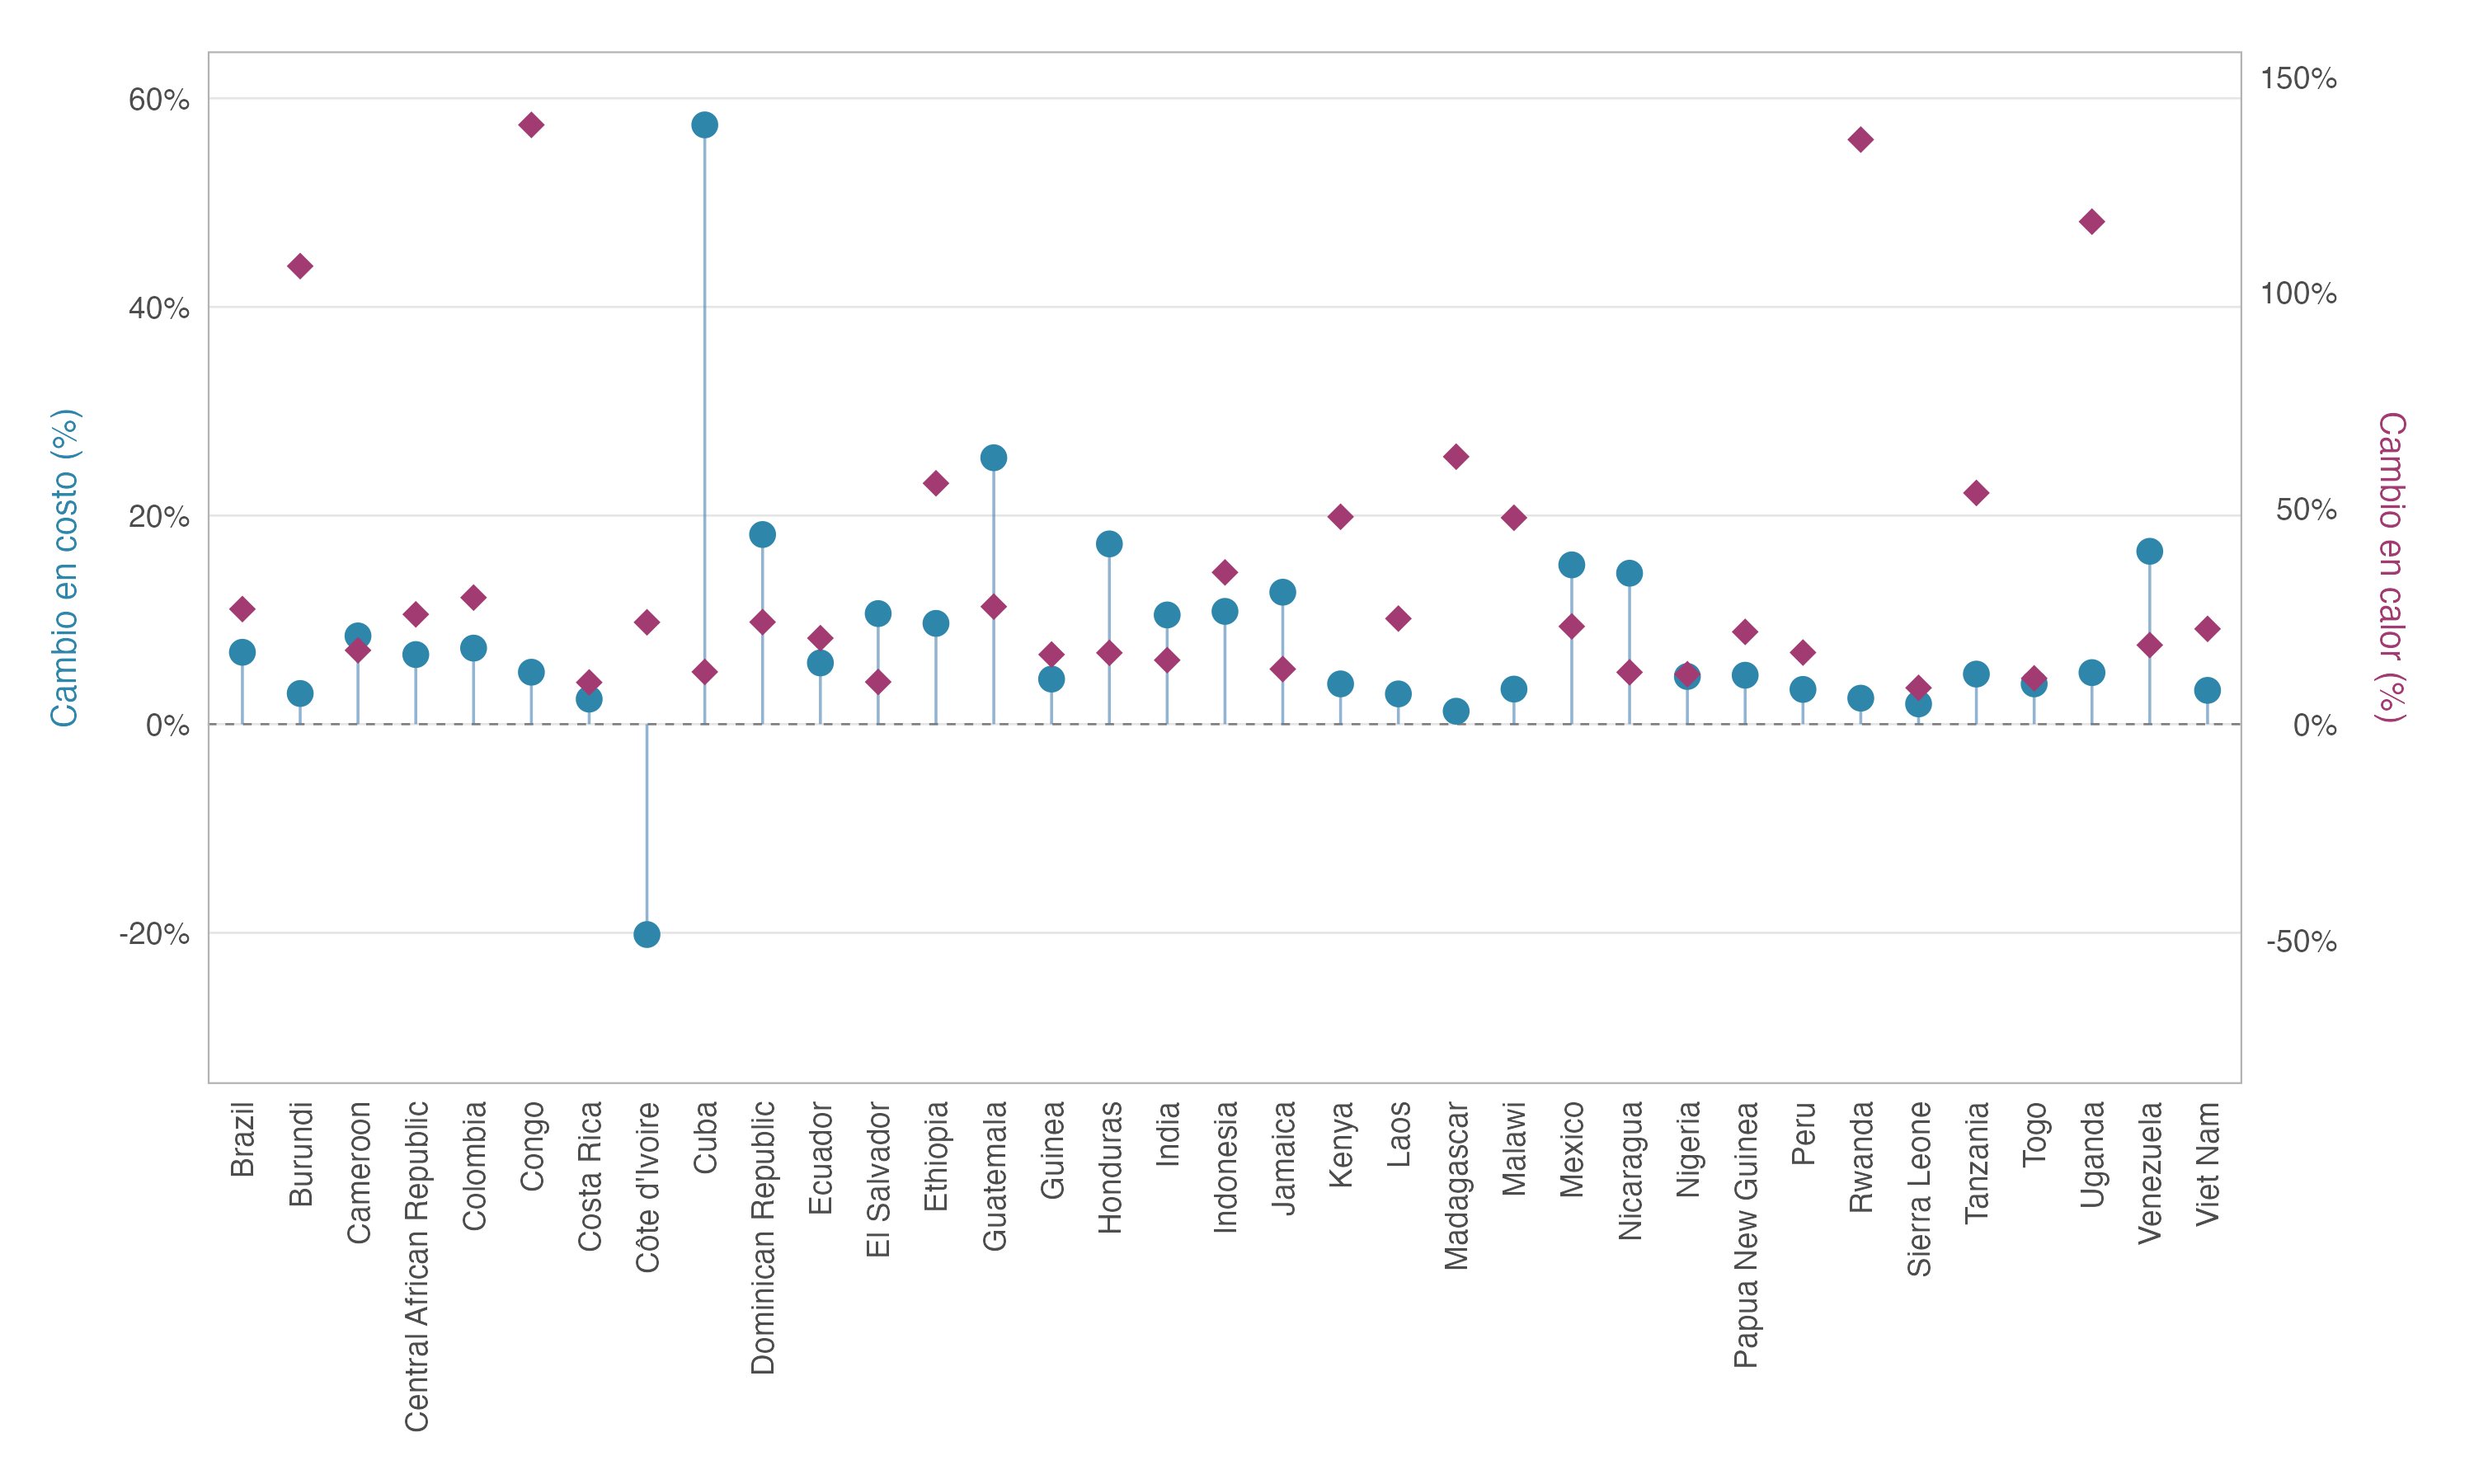
\includegraphics[scale = 0.4]{figures/diff_heat_diff_costs}
    \label{diff_heat_diff_costs}
    \end{figure}
\end{frame}

\begin{frame}{Apéndice}{Cambio en costos y cantidades. Resultados por país \hyperlink{frame:hallazgo2}{\beamerbutton{Volver}}}
    \label{frame:diff_costs_diff_qe}
    \begin{figure}[H]
        \caption{Cambio en costos y cantidades (1990-2019 vs. 1970-1989)}
    \centering
    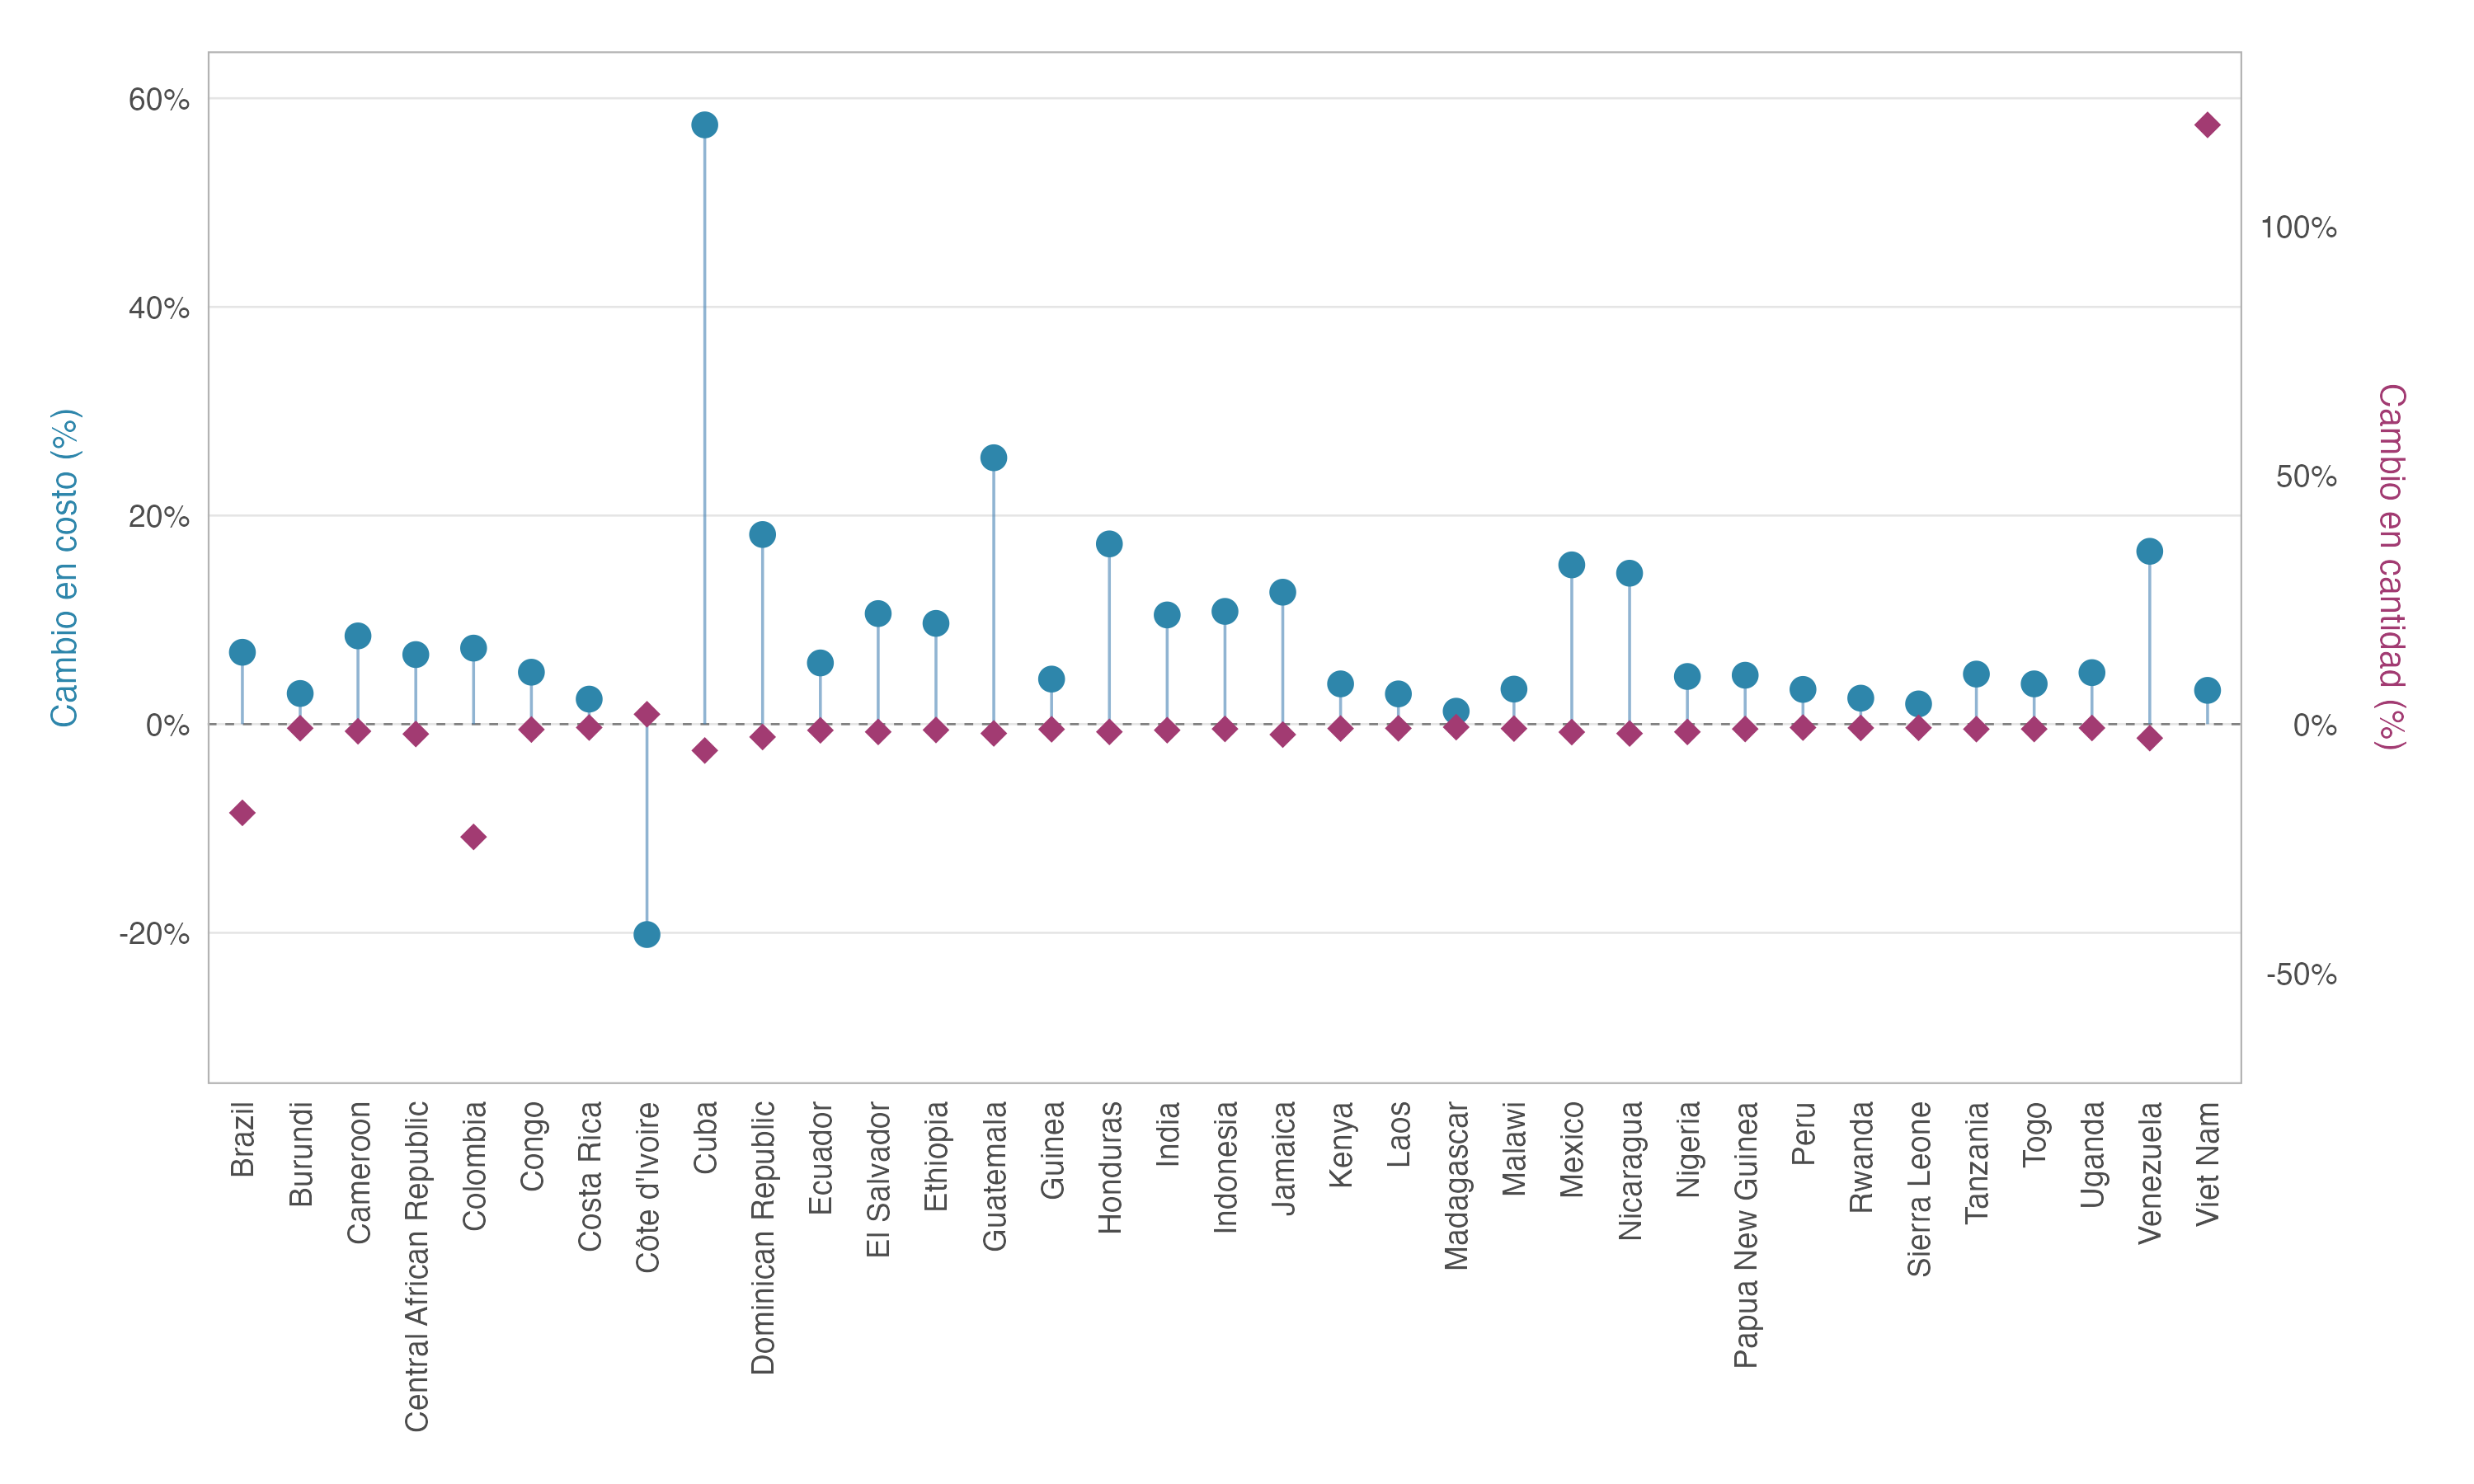
\includegraphics[scale = 0.4]{figures/diff_costs_diff_qe}
    \label{diff_costs_diff_qe}
    \end{figure}
\end{frame}

\begin{frame}{Apéndice}{Cambio en costos y beneficios. Resultados por país \hyperlink{frame:hallazgo2}{\beamerbutton{Volver}}}
    \label{frame:diff_costs_diff_profit}
    \begin{figure}[H]
        \caption{Cambio en costos y beneficios (1990-2019 vs. 1970-1989)}
    \centering
    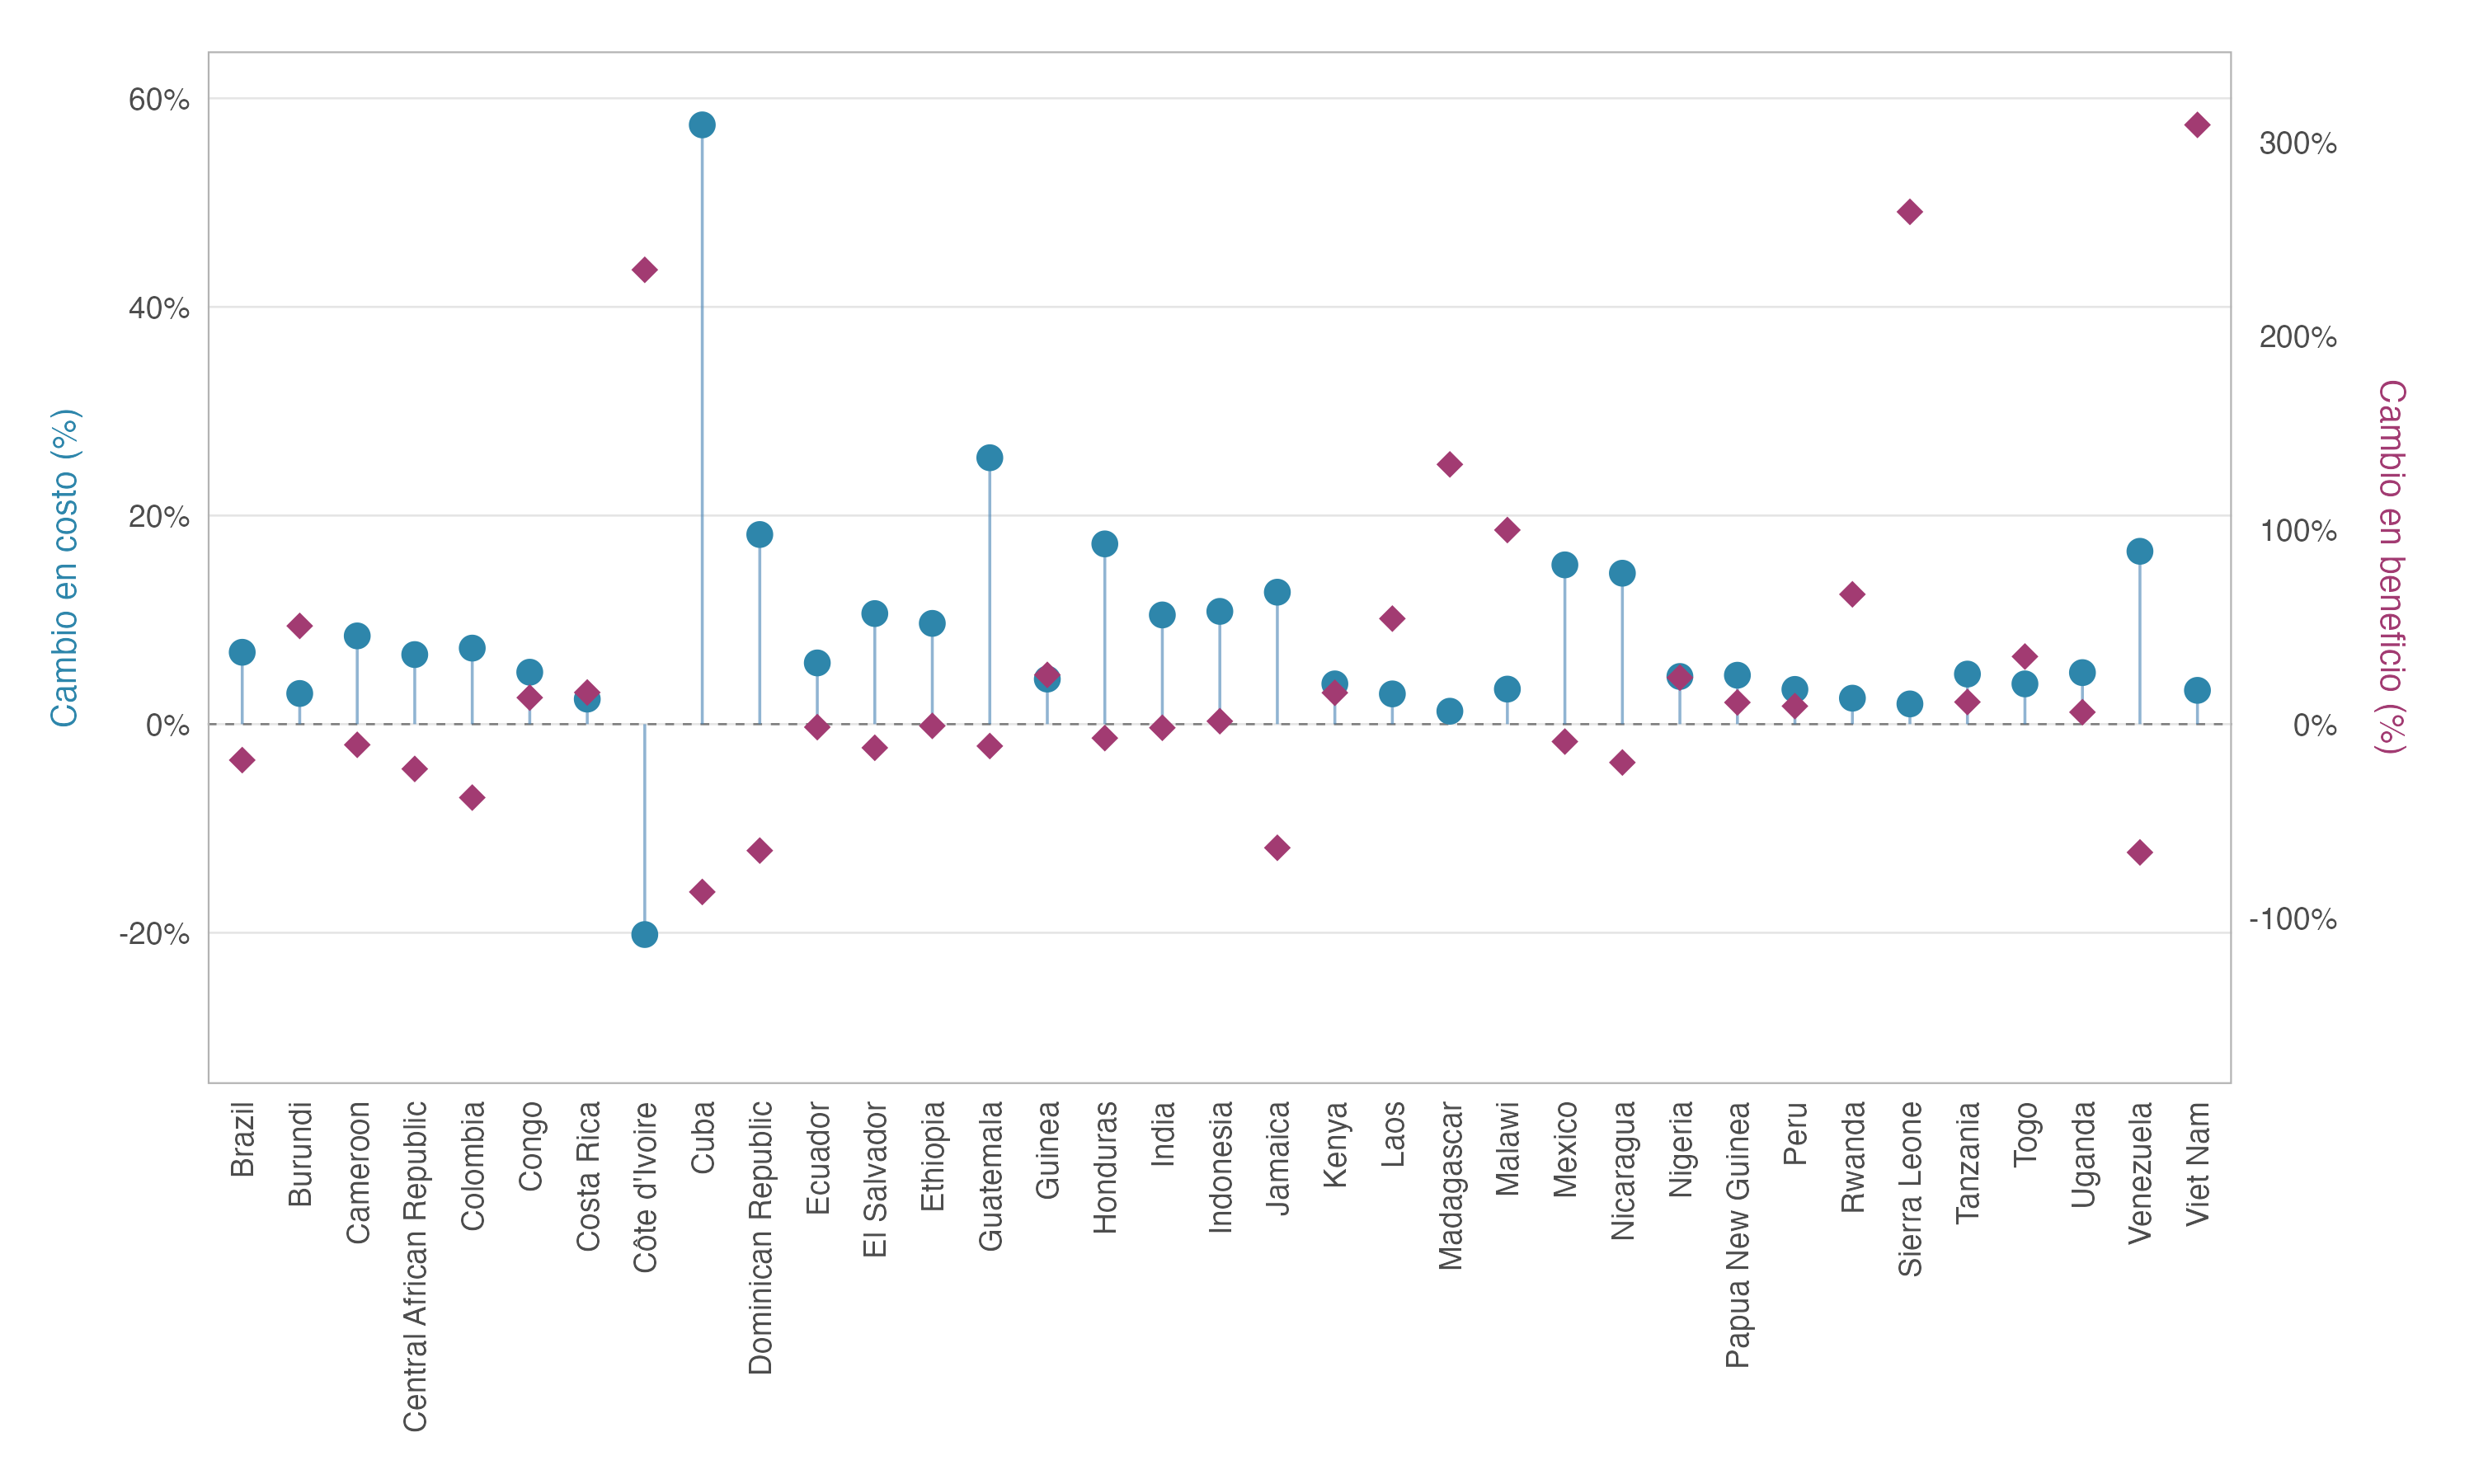
\includegraphics[scale = 0.4]{figures/diff_costs_diff_profit}
    \label{diff_costs_diff_profit}
    \end{figure}
\end{frame}

\begin{frame}{Apéndice}{Descomposición del efecto total \hyperlink{frame:descomposicion1}{\beamerbutton{Volver}}}
    \label{frame:efecto_estrategico1}
    \begin{figure}
    \caption{Efecto estratégico y pérdida. Promedio anualizado (1990-2019)}
    \centering
    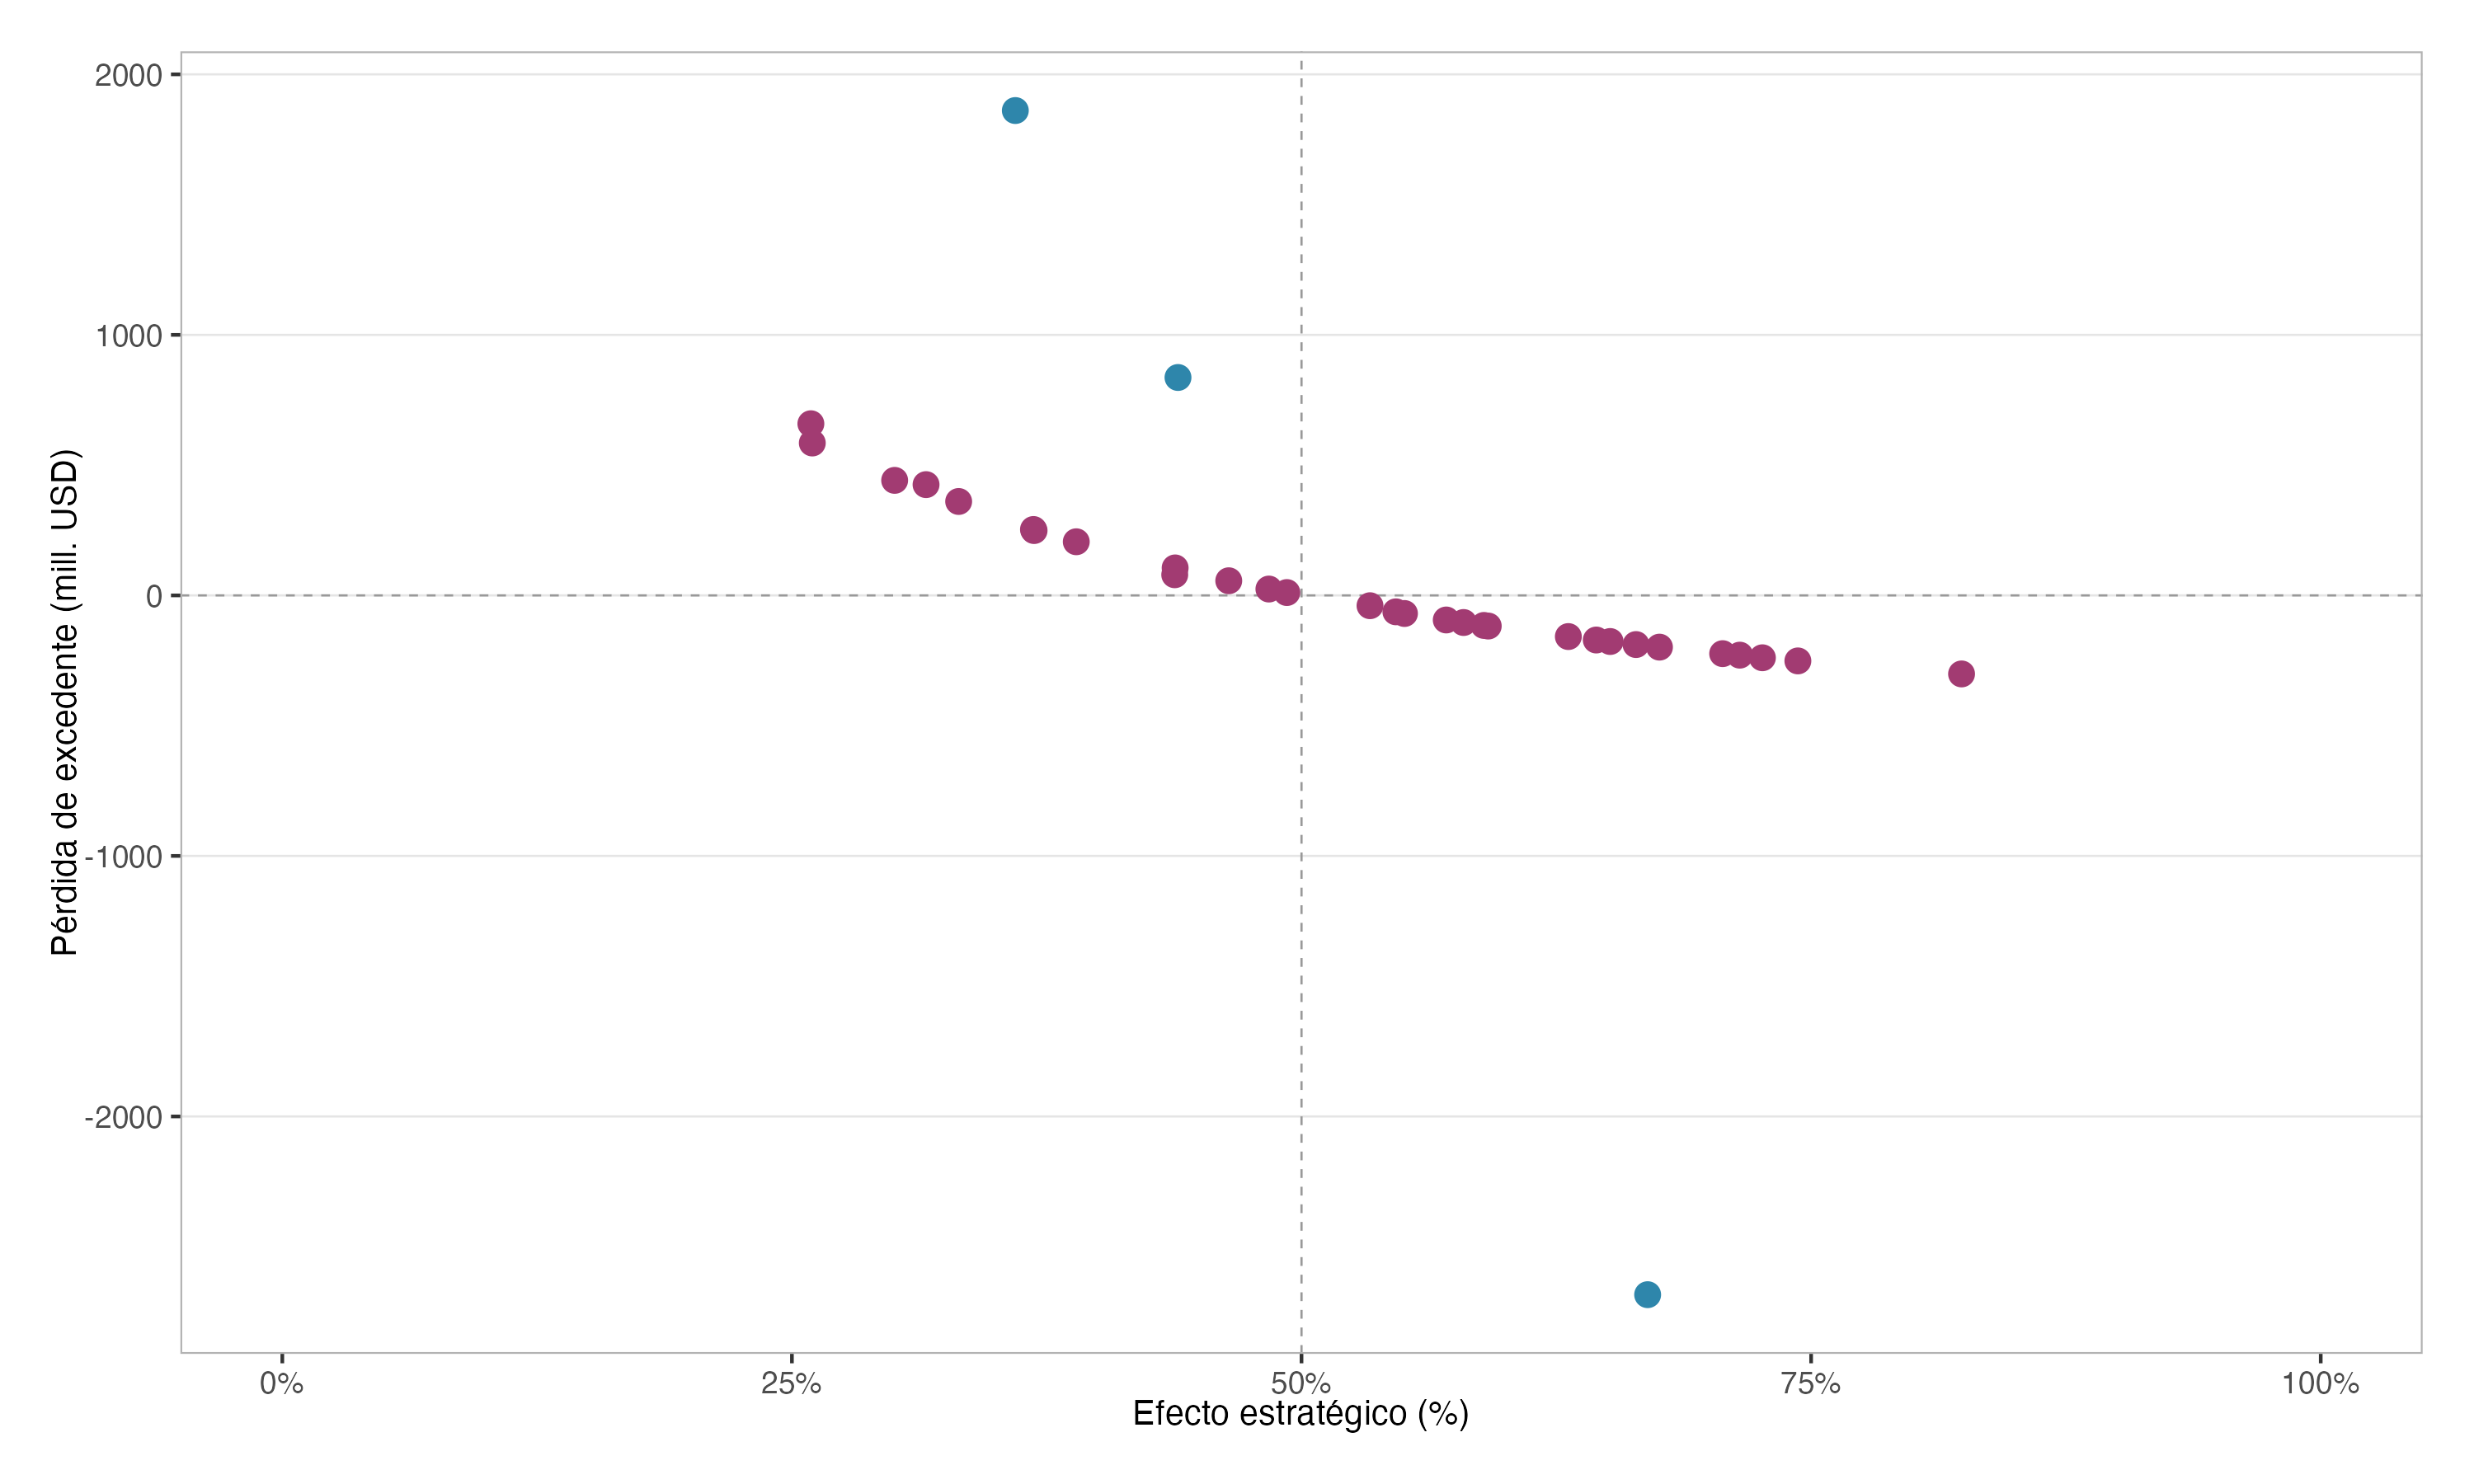
\includegraphics[scale=0.4]{figures/efecto_est_prop_nout}
    \label{efecto_est_prop_nout}
    \end{figure}
\end{frame}
\begin{frame}{Apéndice}{Descomposición del efecto total \hyperlink{frame:descomposicion1}{\beamerbutton{Volver}}}
    \label{frame:efecto_estrategico2}
    \begin{figure}
    \caption{Efecto estratégico y cambio en costos. Promedio anualizado (1990-2019)}
    \centering
    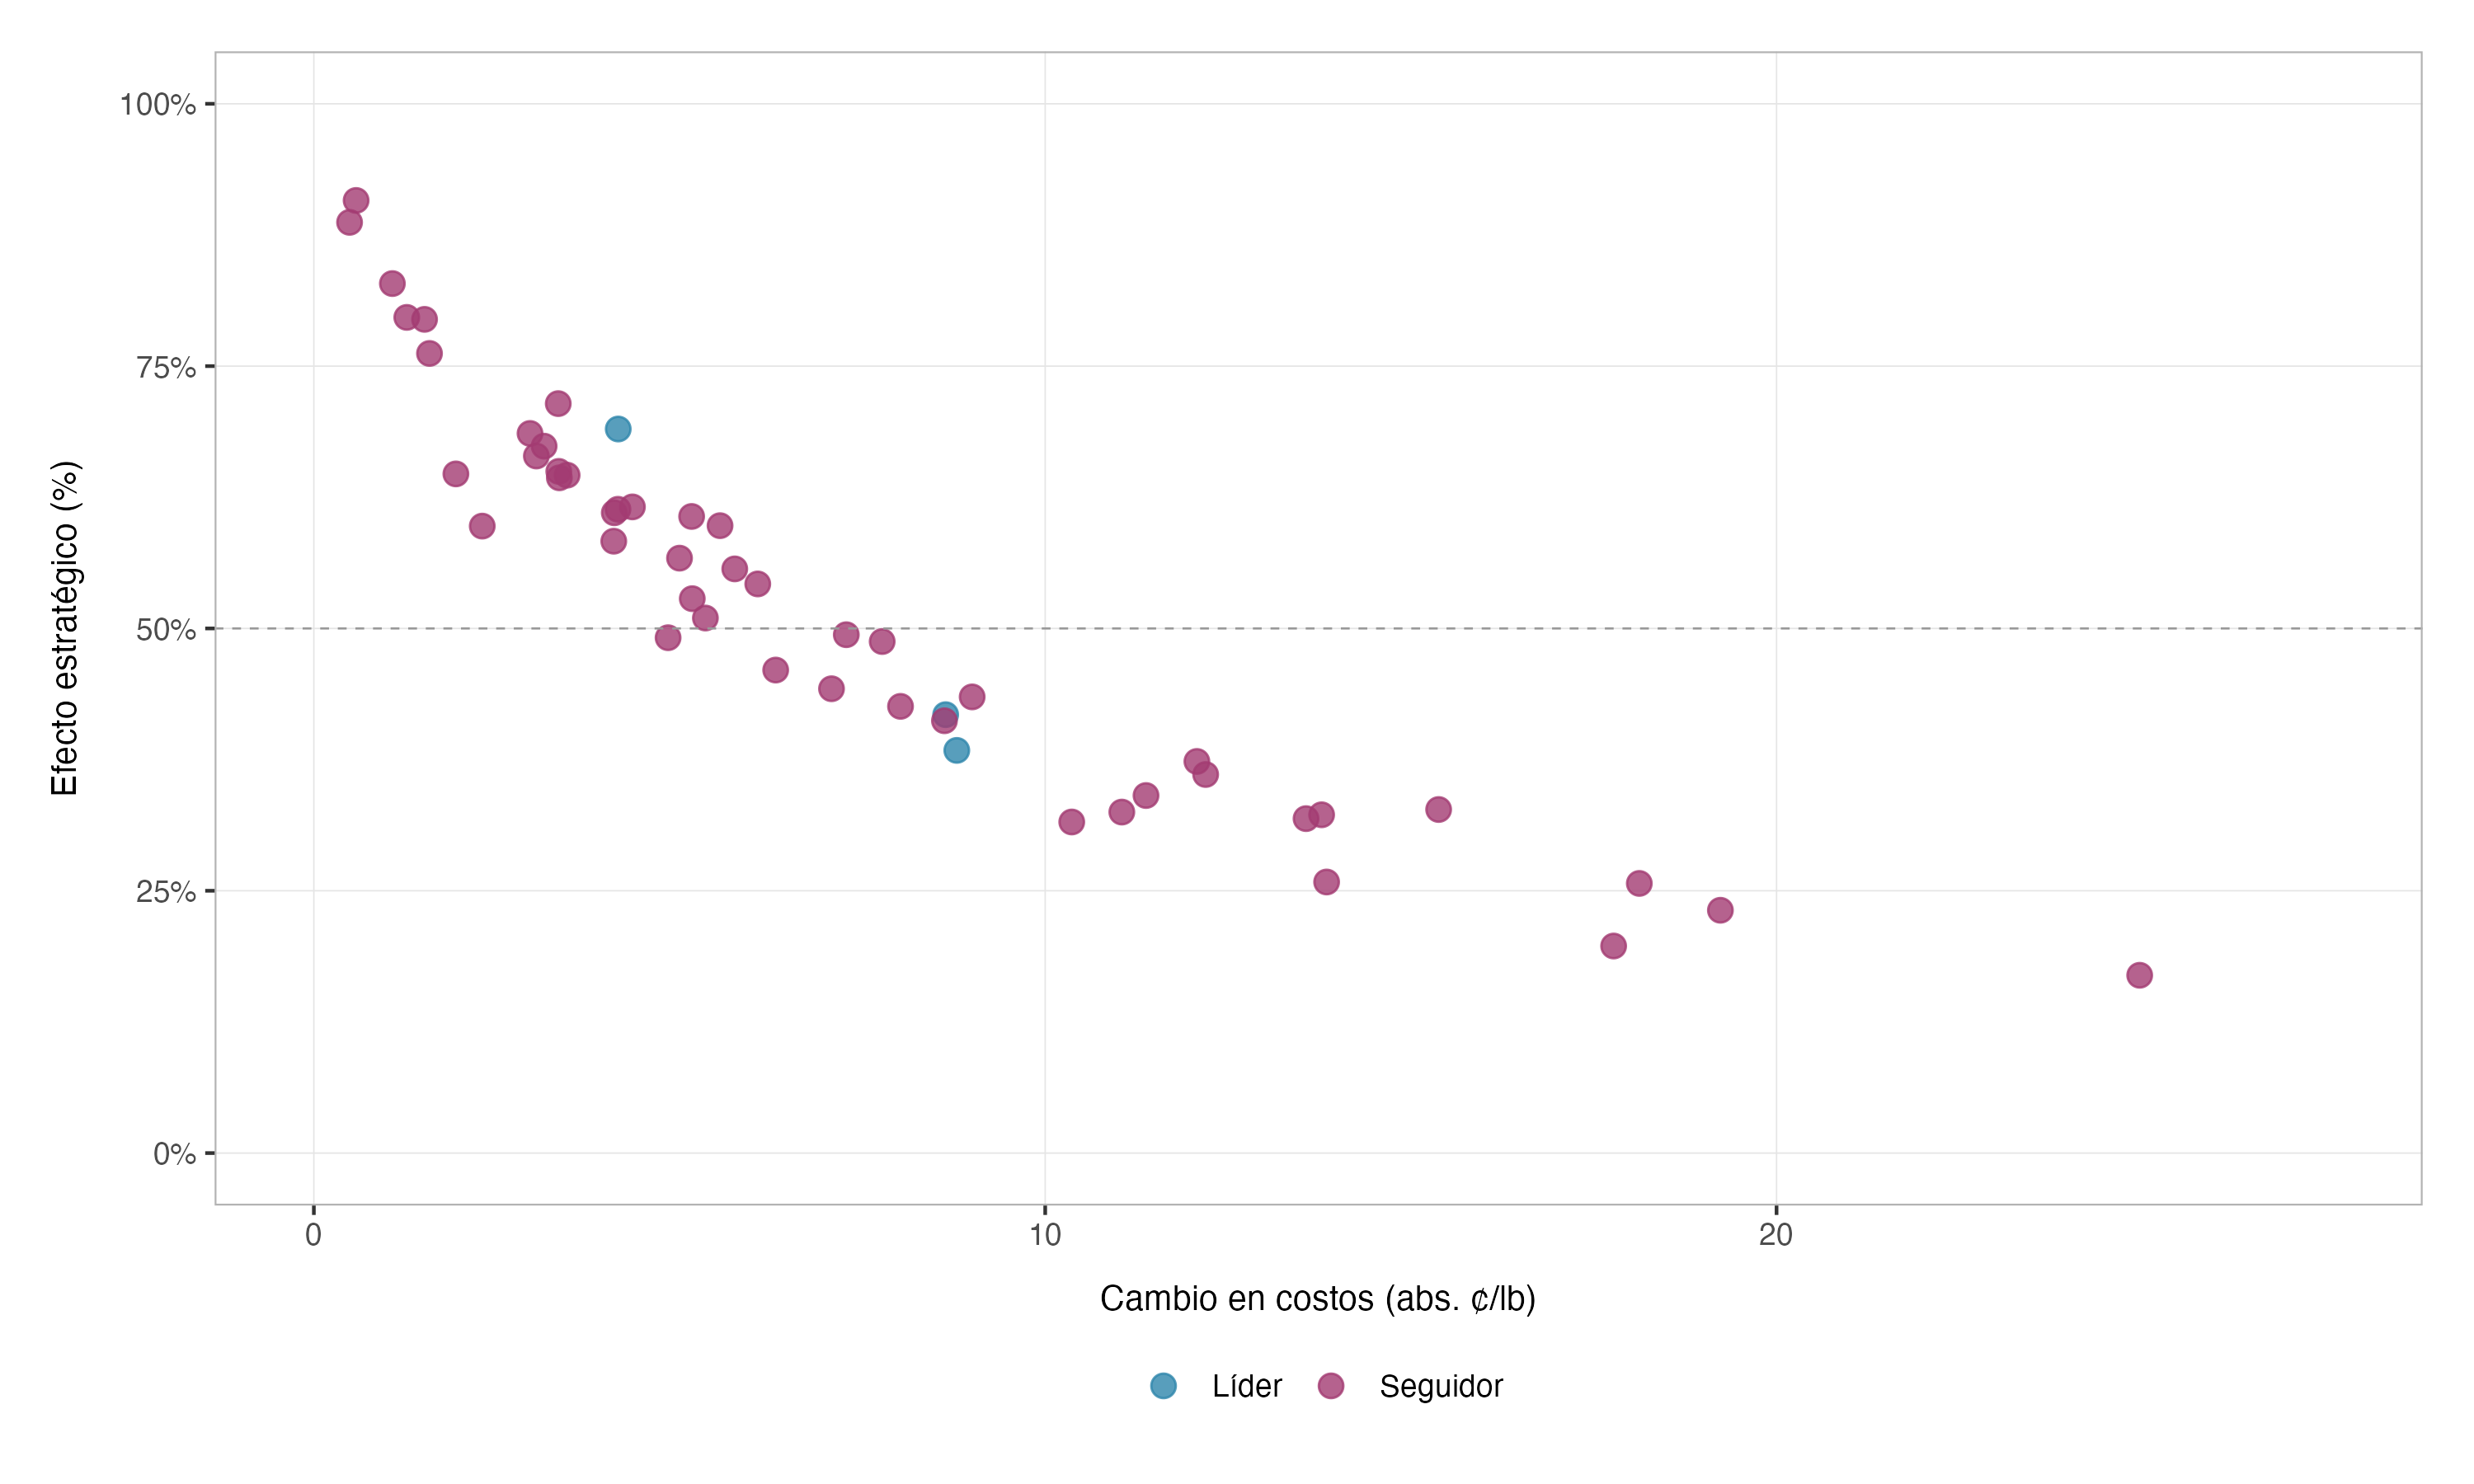
\includegraphics[scale=0.4]{figures/costs_strat}
    \label{costs_strat}
    \end{figure}
\end{frame}
\begin{frame}{Apéndice}{Descomposición del efecto total \hyperlink{frame:descomposicion1}{\beamerbutton{Volver}}}
    \label{frame:efecto_estrategico3}
    \begin{figure}
    \caption{Efecto estratégico y cambio en calor. Promedio anualizado (1990-2019)}
    \centering
    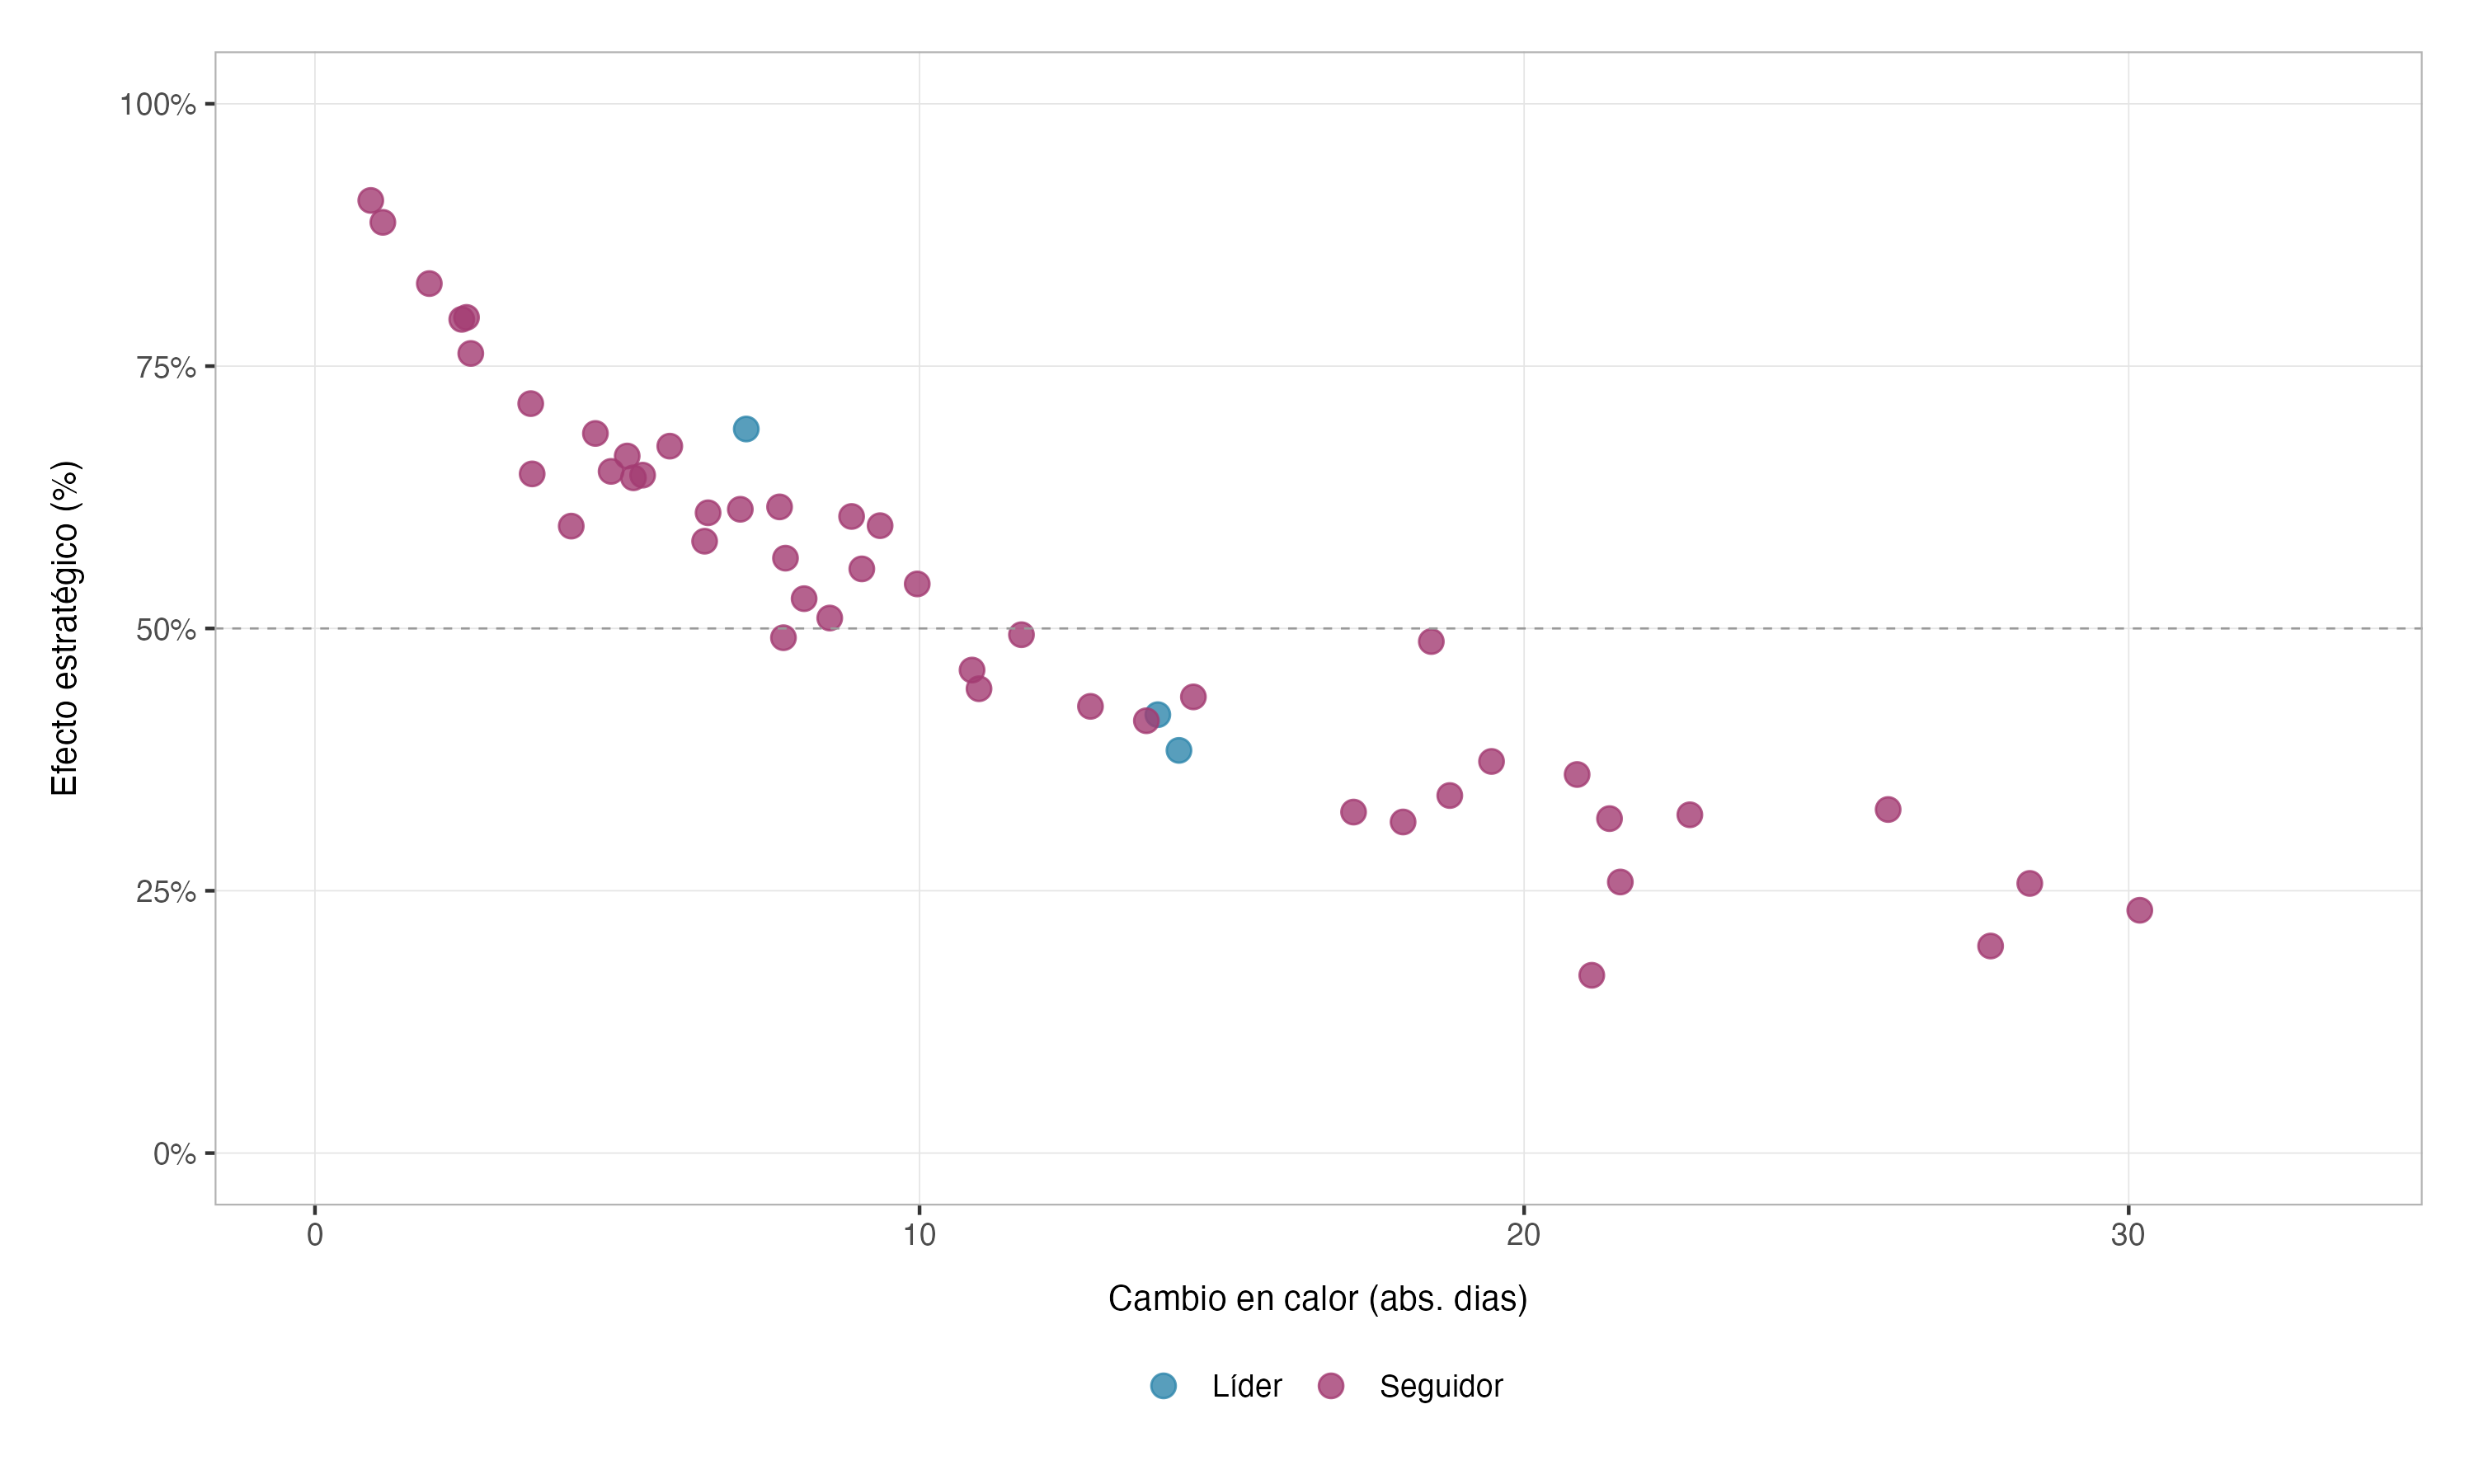
\includegraphics[scale=0.4]{figures/heat_strat}
    \label{heat_strat}
    \end{figure}
\end{frame}


\end{document}